% Options for packages loaded elsewhere
\PassOptionsToPackage{unicode}{hyperref}
\PassOptionsToPackage{hyphens}{url}
\PassOptionsToPackage{dvipsnames,svgnames,x11names}{xcolor}
%
\documentclass[
  12pt,
  oneside]{book}
\usepackage{amsmath,amssymb}
\usepackage{iftex}
\ifPDFTeX
  \usepackage[T1]{fontenc}
  \usepackage[utf8]{inputenc}
  \usepackage{textcomp} % provide euro and other symbols
\else % if luatex or xetex
  \usepackage{unicode-math} % this also loads fontspec
  \defaultfontfeatures{Scale=MatchLowercase}
  \defaultfontfeatures[\rmfamily]{Ligatures=TeX,Scale=1}
\fi
\usepackage{lmodern}
\ifPDFTeX\else
  % xetex/luatex font selection
\fi
% Use upquote if available, for straight quotes in verbatim environments
\IfFileExists{upquote.sty}{\usepackage{upquote}}{}
\IfFileExists{microtype.sty}{% use microtype if available
  \usepackage[]{microtype}
  \UseMicrotypeSet[protrusion]{basicmath} % disable protrusion for tt fonts
}{}
\makeatletter
\@ifundefined{KOMAClassName}{% if non-KOMA class
  \IfFileExists{parskip.sty}{%
    \usepackage{parskip}
  }{% else
    \setlength{\parindent}{0pt}
    \setlength{\parskip}{6pt plus 2pt minus 1pt}}
}{% if KOMA class
  \KOMAoptions{parskip=half}}
\makeatother
\usepackage{xcolor}
\usepackage{color}
\usepackage{fancyvrb}
\newcommand{\VerbBar}{|}
\newcommand{\VERB}{\Verb[commandchars=\\\{\}]}
\DefineVerbatimEnvironment{Highlighting}{Verbatim}{commandchars=\\\{\}}
% Add ',fontsize=\small' for more characters per line
\usepackage{framed}
\definecolor{shadecolor}{RGB}{248,248,248}
\newenvironment{Shaded}{\begin{snugshade}}{\end{snugshade}}
\newcommand{\AlertTok}[1]{\textcolor[rgb]{0.94,0.16,0.16}{#1}}
\newcommand{\AnnotationTok}[1]{\textcolor[rgb]{0.56,0.35,0.01}{\textbf{\textit{#1}}}}
\newcommand{\AttributeTok}[1]{\textcolor[rgb]{0.13,0.29,0.53}{#1}}
\newcommand{\BaseNTok}[1]{\textcolor[rgb]{0.00,0.00,0.81}{#1}}
\newcommand{\BuiltInTok}[1]{#1}
\newcommand{\CharTok}[1]{\textcolor[rgb]{0.31,0.60,0.02}{#1}}
\newcommand{\CommentTok}[1]{\textcolor[rgb]{0.56,0.35,0.01}{\textit{#1}}}
\newcommand{\CommentVarTok}[1]{\textcolor[rgb]{0.56,0.35,0.01}{\textbf{\textit{#1}}}}
\newcommand{\ConstantTok}[1]{\textcolor[rgb]{0.56,0.35,0.01}{#1}}
\newcommand{\ControlFlowTok}[1]{\textcolor[rgb]{0.13,0.29,0.53}{\textbf{#1}}}
\newcommand{\DataTypeTok}[1]{\textcolor[rgb]{0.13,0.29,0.53}{#1}}
\newcommand{\DecValTok}[1]{\textcolor[rgb]{0.00,0.00,0.81}{#1}}
\newcommand{\DocumentationTok}[1]{\textcolor[rgb]{0.56,0.35,0.01}{\textbf{\textit{#1}}}}
\newcommand{\ErrorTok}[1]{\textcolor[rgb]{0.64,0.00,0.00}{\textbf{#1}}}
\newcommand{\ExtensionTok}[1]{#1}
\newcommand{\FloatTok}[1]{\textcolor[rgb]{0.00,0.00,0.81}{#1}}
\newcommand{\FunctionTok}[1]{\textcolor[rgb]{0.13,0.29,0.53}{\textbf{#1}}}
\newcommand{\ImportTok}[1]{#1}
\newcommand{\InformationTok}[1]{\textcolor[rgb]{0.56,0.35,0.01}{\textbf{\textit{#1}}}}
\newcommand{\KeywordTok}[1]{\textcolor[rgb]{0.13,0.29,0.53}{\textbf{#1}}}
\newcommand{\NormalTok}[1]{#1}
\newcommand{\OperatorTok}[1]{\textcolor[rgb]{0.81,0.36,0.00}{\textbf{#1}}}
\newcommand{\OtherTok}[1]{\textcolor[rgb]{0.56,0.35,0.01}{#1}}
\newcommand{\PreprocessorTok}[1]{\textcolor[rgb]{0.56,0.35,0.01}{\textit{#1}}}
\newcommand{\RegionMarkerTok}[1]{#1}
\newcommand{\SpecialCharTok}[1]{\textcolor[rgb]{0.81,0.36,0.00}{\textbf{#1}}}
\newcommand{\SpecialStringTok}[1]{\textcolor[rgb]{0.31,0.60,0.02}{#1}}
\newcommand{\StringTok}[1]{\textcolor[rgb]{0.31,0.60,0.02}{#1}}
\newcommand{\VariableTok}[1]{\textcolor[rgb]{0.00,0.00,0.00}{#1}}
\newcommand{\VerbatimStringTok}[1]{\textcolor[rgb]{0.31,0.60,0.02}{#1}}
\newcommand{\WarningTok}[1]{\textcolor[rgb]{0.56,0.35,0.01}{\textbf{\textit{#1}}}}
\usepackage{longtable,booktabs,array}
\usepackage{calc} % for calculating minipage widths
% Correct order of tables after \paragraph or \subparagraph
\usepackage{etoolbox}
\makeatletter
\patchcmd\longtable{\par}{\if@noskipsec\mbox{}\fi\par}{}{}
\makeatother
% Allow footnotes in longtable head/foot
\IfFileExists{footnotehyper.sty}{\usepackage{footnotehyper}}{\usepackage{footnote}}
\makesavenoteenv{longtable}
\usepackage{graphicx}
\makeatletter
\def\maxwidth{\ifdim\Gin@nat@width>\linewidth\linewidth\else\Gin@nat@width\fi}
\def\maxheight{\ifdim\Gin@nat@height>\textheight\textheight\else\Gin@nat@height\fi}
\makeatother
% Scale images if necessary, so that they will not overflow the page
% margins by default, and it is still possible to overwrite the defaults
% using explicit options in \includegraphics[width, height, ...]{}
\setkeys{Gin}{width=\maxwidth,height=\maxheight,keepaspectratio}
% Set default figure placement to htbp
\makeatletter
\def\fps@figure{htbp}
\makeatother
\setlength{\emergencystretch}{3em} % prevent overfull lines
\providecommand{\tightlist}{%
  \setlength{\itemsep}{0pt}\setlength{\parskip}{0pt}}
\setcounter{secnumdepth}{5}
\usepackage{booktabs,multirow,color,eurosym}
\usepackage{amsthm}
\usepackage{multicol}
\usepackage{geometry}
\usepackage[natbibapa]{apacite}
% \usepackage{txfonts} %txfonts iwona lmodern
\usepackage{hyperref}

\usepackage{lmodern}
\usepackage[T1]{fontenc}

\renewcommand{\texteuro}{\text{\euro}} 
%\hypersetup{colorlinks=false, pdfborderstyle={/S/U/W 1} }

%\geometry{executivepaper}
\geometry{a4paper}
\usepackage{makeidx}
%\usepackage{imakeidx} % Uncomment to get correct page numbers in index
\makeindex




%% Note: Pandoc (which is doing all of the output conversion behind the scenes) does not parse the content of LaTeX environments. This creates problems when you try to include LaTeX commands with curly brackets directly in your Rmd file. E.g. You can't just use `\begin{multicols}{2}` directly in your Rmd file. Luckily, a straightforward workaround is to simply define some new shortcut commands yourself as per the below.
%% See: https://stackoverflow.com/questions/25849814/rstudio-rmarkdown-both-portrait-and-landscape-layout-in-a-single-pdf/27334272#27334272
\newcommand{\btwocol}{\begin{multicols}{2}}
\newcommand{\etwocol}{\end{multicols}}

\usepackage{caption}
\captionsetup[table]{labelformat=empty}
\usepackage{tikz}
\ifLuaTeX
  \usepackage{selnolig}  % disable illegal ligatures
\fi
\usepackage[]{natbib}
\bibliographystyle{plainnat}
\IfFileExists{bookmark.sty}{\usepackage{bookmark}}{\usepackage{hyperref}}
\IfFileExists{xurl.sty}{\usepackage{xurl}}{} % add URL line breaks if available
\urlstyle{same}
\hypersetup{
  pdftitle={ How to Use R for Data Science},
  pdfauthor={© Prof.~Dr.~Stephan Huber (Stephan.Huber@hs-fresenius.de)},
  colorlinks=true,
  linkcolor={red},
  filecolor={Maroon},
  citecolor={Blue},
  urlcolor={blue},
  pdfcreator={LaTeX via pandoc}}

\title{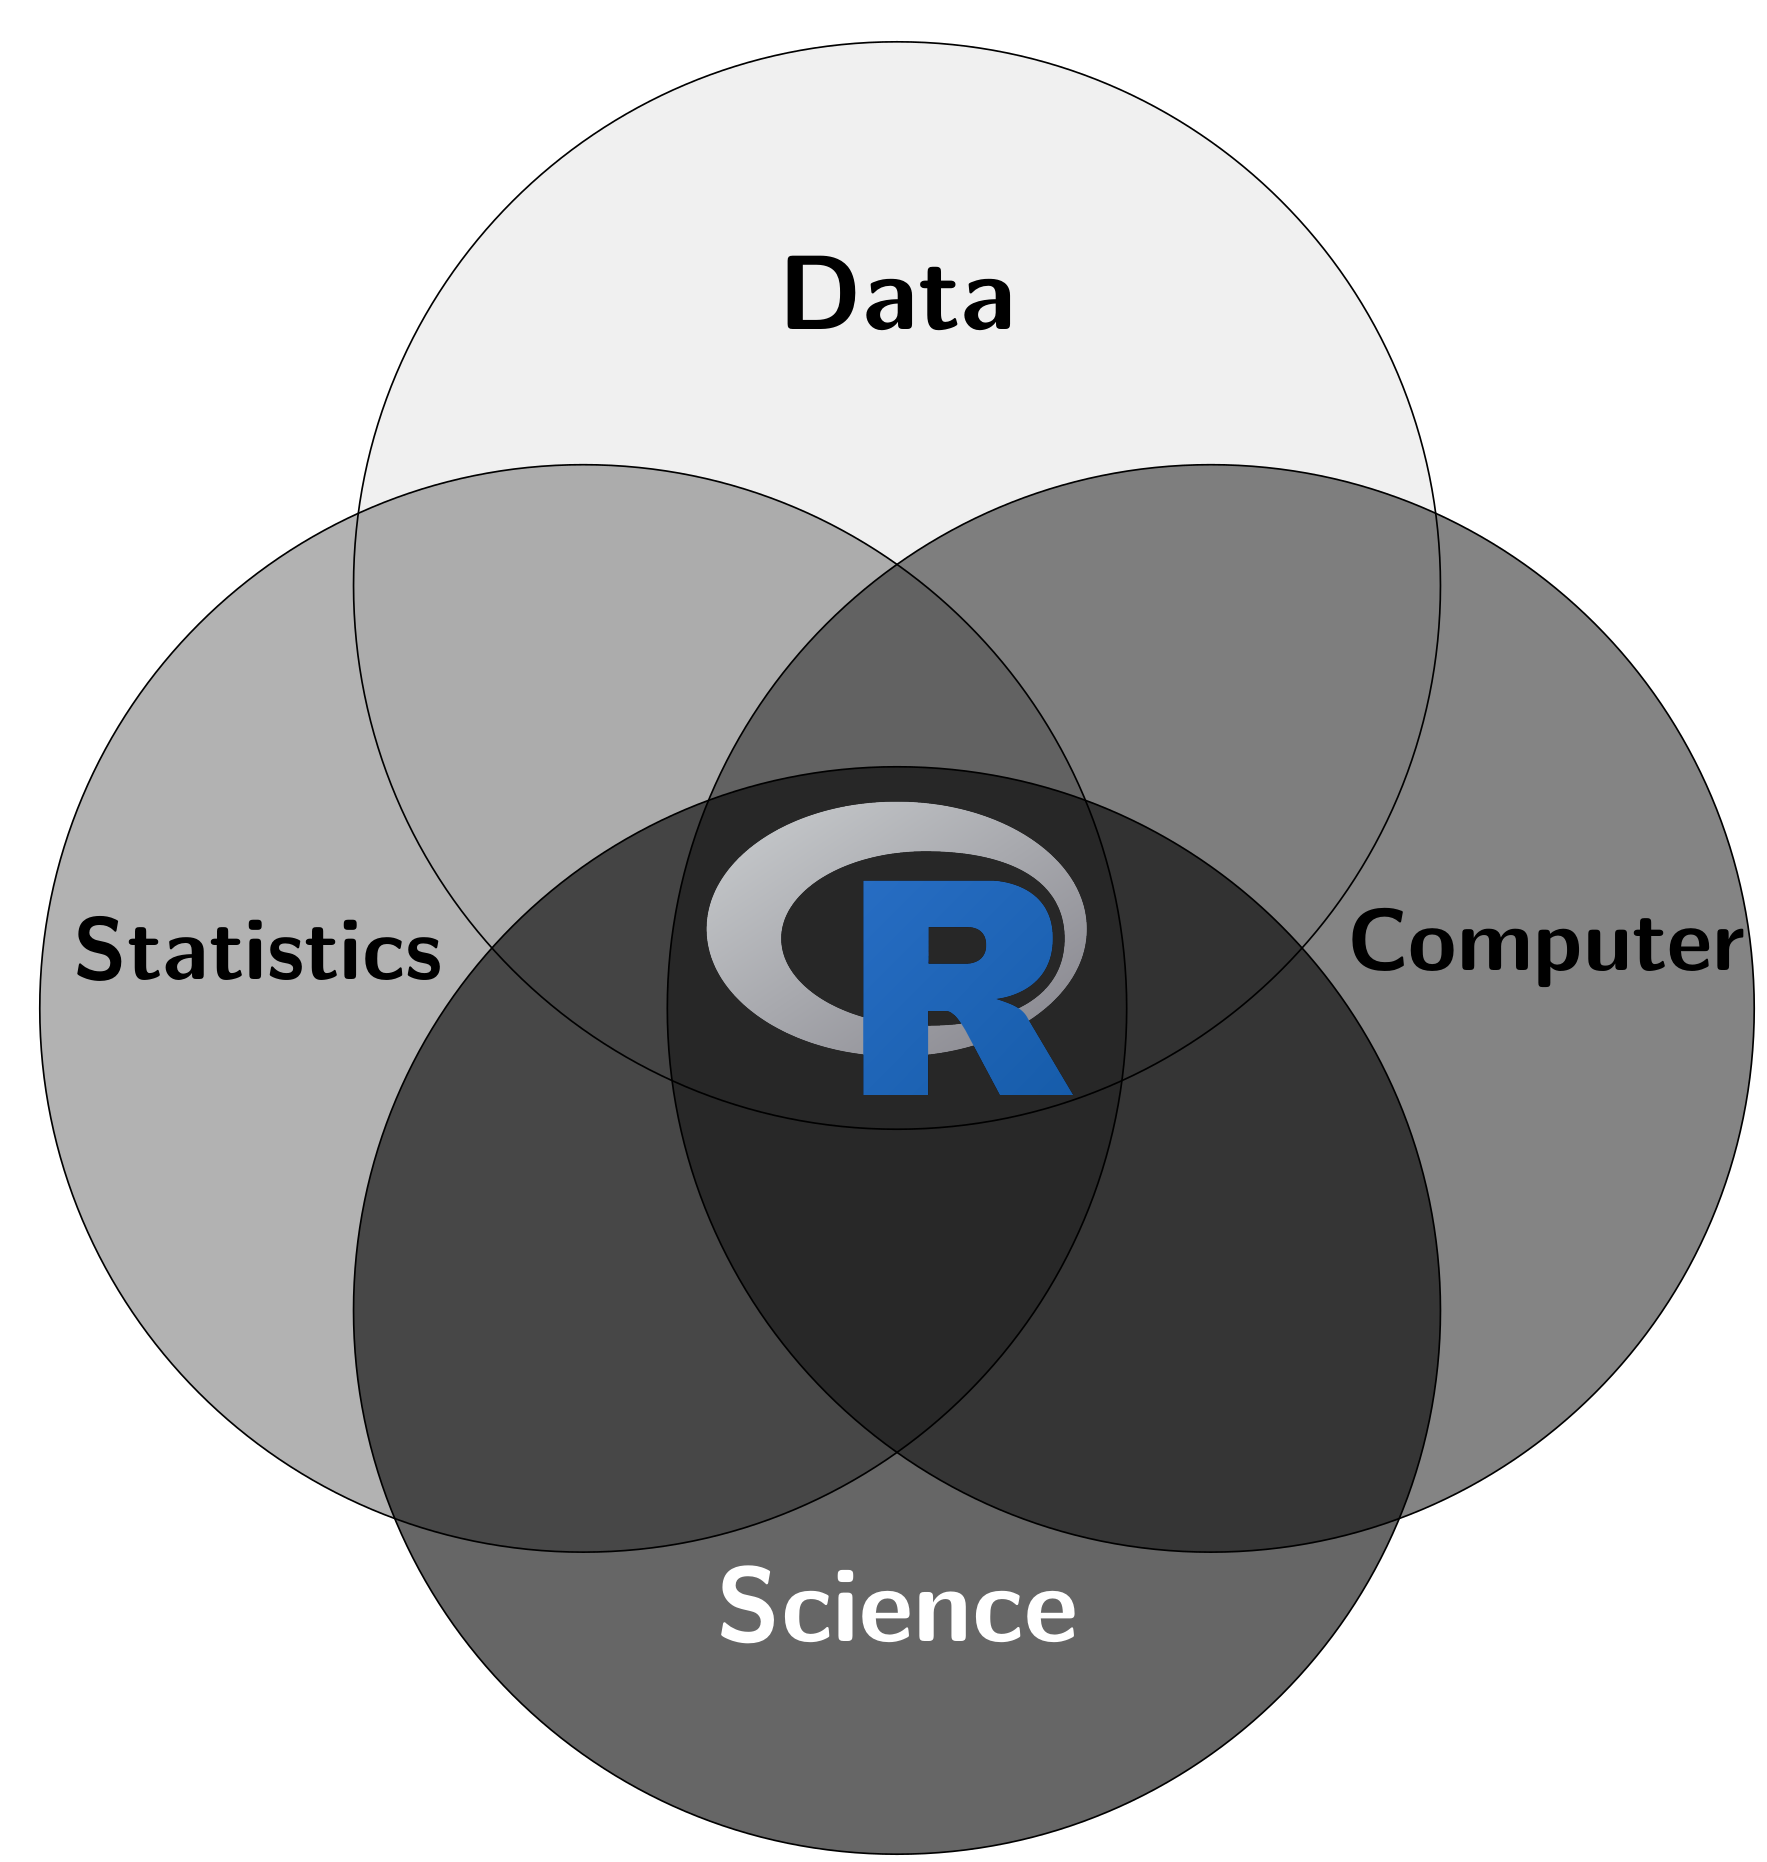
\includegraphics[width=8cm,height=\textheight]{fig/cover.png}\\
How to Use R for Data Science}
\usepackage{etoolbox}
\makeatletter
\providecommand{\subtitle}[1]{% add subtitle to \maketitle
  \apptocmd{\@title}{\par {\large #1 \par}}{}{}
}
\makeatother
\subtitle{Lecture Notes}
\author{© Prof.~Dr.~Stephan Huber (\href{mailto:Stephan.Huber@hs-fresenius.de}{\nolinkurl{Stephan.Huber@hs-fresenius.de}})}
\date{Last compiled on 15 November, 2023}

\usepackage{amsthm}
\newtheorem{theorem}{Theorem}[chapter]
\newtheorem{lemma}{Lemma}[chapter]
\newtheorem{corollary}{Corollary}[chapter]
\newtheorem{proposition}{Proposition}[chapter]
\newtheorem{conjecture}{Conjecture}[chapter]
\theoremstyle{definition}
\newtheorem{definition}{Definition}[chapter]
\theoremstyle{definition}
\newtheorem{example}{Example}[chapter]
\theoremstyle{definition}
\newtheorem{exercise}{Exercise}[chapter]
\theoremstyle{definition}
\newtheorem{hypothesis}{Hypothesis}[chapter]
\theoremstyle{remark}
\newtheorem*{remark}{Remark}
\newtheorem*{solution}{Solution}
\begin{document}
\maketitle

{
\hypersetup{linkcolor=}
\setcounter{tocdepth}{2}
\tableofcontents
}
\hypertarget{preface}{%
\chapter*{Preface}\label{preface}}
\addcontentsline{toc}{chapter}{Preface}

While data science is an appealing buzzword that combines different fields of knowledge such as computer science, software engineering, informatics, database management, statistics, econometrics, business intelligence, and mathematics, there is no universally accepted definition of it and I think it is not important to define it precisely. \citet[p.~97]{Kelleher2018Data} wrote ``Data science is best understood as a partnership between a data scientist and a computer.'' So data science is about embracing the power of computers for scientific, commercial or social purposes. Of course, empirical models and statistics play a role in gaining meaningful insights. The graphic on the cover page may illustrate that R combines four important fields, that are, data, science, computer, and statistics.

The programming language R allows you to manipulate, visualize, and analyze data. It works on different operating systems (Windows, Mac, Linux) and can do a lot of things better than other programs (Python, Stata, Eviews, SPSS, SAS, Excel, etc.). R is open source and widely used. This facilitates the
entry enormously. Nevertheless, learning the command syntax is essential for advanced data analysis.
data analysis.

I began my journey into data science in 2003 with the introductory course Statistics by \href{https://scholar.google.com/citations?user=geLs3JUAAAAJ\&hl=en}{Daniel Rösch}. I learned a lot. In particular, that probabilities often play a role when analyzing data. After that, I joined \href{https://scholar.google.ca/citations?user=tHNB7wIAAAAJ\&hl=en}{Harry Haupt's} \emph{Introductory Econometrics} course, where I studied the infamous Jeffrey M. \citet{Wooldridge2002Introductory} textbook. It got me hooked and I took all the courses \href{https://www.uni-regensburg.de/business-economics-and-management-information-systems/economics-tschernig/team/rolf-tschernig/index.html}{Rolf Tschernig} offered at his chair of Econometrics, where I became a tutor at the University of Regensburg and a research assistant of \href{https://iab.de/en/employee/m\%C3\%B6ller-joachim/}{Joachim Möller}. Despite everything we did had to do with how to make sense out of data, we never actually used the term \emph{data science} which is also absent in the more 850 pages long textbook by \citet{Wooldridge2002Introductory}. The book also remains silent about \emph{machine learning} or \emph{artificial intelligence}. These terms became popular only after I graduated. The \emph{Harvard Business Review} article by \citet{Davenport2012Data} who claimed that data scientist is ``The Sexiest Job of the 21st Century'' may have boosted the popularity.

This makes me wonder if I can call myself a data scientist and why so many of my former comolitons, colleagues, and students call themselves now data scientists even though the term basically played no role in our education.

\hypertarget{about-the-lecture-notes}{%
\section*{About the lecture notes}\label{about-the-lecture-notes}}

\begin{itemize}
\tightlist
\item
  These notes aims to support my lecture at the HS Fresenius but are incomplete and no substitute for taking actively part in class.
\item
  A pdf version of these notes is available \href{https://raw.githubusercontent.com/hubchev/hubchev.github.io/main/ds/_main.pdf}{here}
\item
  I host the notes in a \href{https://github.com/hubchev/hubchev.github.io/tree/main/ds}{GitHub repo}.
\item
  I appreciate you reading it, and I appreciate any comments.
\item
  This is work in progress so please check for updates regularly.
\item
  These notes are published under a Creative Commons BY-SA license (CC BY-SA) version 4.0. This means it can be reused, remixed, retained, revised and redistributed as long as appropriate credit is given to the authors. If you remix, or modify the original version of this open textbook, you must redistribute all versions of this open textbook under the same license---CC BY-SA. This script is build on the work of \citet{Navarro2020Learning}, \citet{Muschelli2022Introduction}, \citet{Thulin2021Modern}, and \citet{Ismay2022Statistical} which is also published under CC BY-SA.
\end{itemize}

\hypertarget{about-the-author}{%
\section*{About the author}\label{about-the-author}}

\begin{figure}
\centering

\includegraphics[width=0.25\textwidth,height=\textheight]{fig/huber2.jpeg}
\caption{\label{fig:itsme} Prof.~Dr.~Stephan Huber}
\end{figure}

I am a Professor of International Economics and Data Science at HS Fresenius, holding a Diploma in Economics from the University of Regensburg and a Doctoral Degree (summa cum laude) from the University of Trier. I completed postgraduate studies at the Interdisciplinary Graduate Center of Excellence at the Institute for Labor Law and Industrial Relations in the European Union (IAAEU) in Trier. Prior to my current position, I worked as a research assistant to Prof.~Dr.~Dr.~h.c. Joachim Möller at the University of Regensburg, a post-doc at the Leibniz Institute for East and Southeast European Studies (IOS) in Regensburg, and a freelancer at Charles University in Prague.

Throughout my career, I have also worked as a lecturer at various institutions, including the TU Munich, the University of Regensburg, Saarland University, and the Universities of Applied Sciences in Frankfurt and Augsburg. Additionally, I have had the opportunity to teach abroad for the University of Cordoba in Spain and the University of Perugia. My published work can be found in international journals such as the Canadian Journal of Economics and the Stata Journal. For more information on my work, please visit my private homepage at \href{www.hubchev.github.io}{hubchev.github.io}.

\textbf{Contact}

\begin{verbatim}
   Hochschule Fresenius für Wirtschaft & Medien GmbH
   Im MediaPark 4c
   50670 Cologne
   
   Office: 4b OG-1 Bü01 
   Telefon: +49 221 973199-523
   Mail: stephan.huber@hs-fresenius.de
   Private homepage: www.hubchev.github.io
   Github: https://github.com/hubchev
\end{verbatim}

\hypertarget{getting-started}{%
\chapter{Getting started with R}\label{getting-started}}

Before we can start exploring data in R, there are some key concepts to understand first:

\begin{enumerate}
\def\labelenumi{\arabic{enumi}.}
\tightlist
\item
  Why R?
\item
  How to learn R?
\item
  What are R and RStudio?
\item
  How to use R and RStudio without installation
\item
  How to install R and RStudio
\item
  How to write and run code in R
\item
  What are R packages?
\item
  What is a function in R?
\item
  What are objects in R?
\item
  Are there some guidelines for working with R?
\end{enumerate}

\hypertarget{sec:whyR}{%
\section{Why R?}\label{sec:whyR}}

R is a free and open-source programming language that provides a wide range of advanced statistics capabilities, state-of-the-art graphics, and powerful data manipulation capabilities. It supports larger data sets, reads any type of data, and runs on multiple platforms. R makes it easier to automate tasks, organize projects, ensure reproducibility, and find and fix errors, and anyone can contribute packages to improve its functionality. Moreover, the following points are worth to emphasize:

\begin{itemize}
\tightlist
\item
  \textbf{R is an artist!} Check out:

  \begin{itemize}
  \tightlist
  \item
    \url{https://www.r-graph-gallery.com/}
  \item
    \url{http://r-statistics.co/Top50-Ggplot2-Visualizations-MasterList-R-Code.html}
  \item
    \url{https://www.r-bloggers.com/2020/05/7-useful-interactive-charts-in-r/}
  \end{itemize}
\item
  \textbf{R is an employment insurance.} If you are good in R programming or if you are good in writing programming code in general, you have plenty of opportunities to earn a decent salary.
\item
  \textbf{R uses the computer and computers are great!} Doing statistics on a computer is faster, easier and more powerful than doing it by hand. Computers excel at mindless repetitive tasks. For most people, the only reason to ever do statistical calculations with pencil and paper is for learning purposes.
\item
  \textbf{Excel is bad!} Doing statistics in a spreadsheet (e.g., Microsoft Excel) is often a bad idea. Although many people are likely feel more familiar with them, spreadsheets are very limited in terms of what analyses they allow you to do. You can easily lose the overview and it is hard to keep track of what you have done and in comparison with command line driven programs. In particular, the ability to make your analysis \emph{replicable} is limited.
\item
  \textbf{R is good, proprietary software is bad!} Avoiding proprietary software is a very good idea because it costly, support is exclusively provided by the owner of the software (if they stop supporting your version you are lost), security issues cannot be checked as the source code is not available, and possibilities for customization are limited.
\item
  \textbf{R is big!} Something that you might not appreciate now, but will love later on if you do anything involving data analysis, is the fact that R is highly extensible. When you download and install R, you get all the basic packages, and those are very powerful on their own. However, because R is so open and so widely used, it's become something of a standard tool in statistics, and so lots of people write their own packages that extend the system. And these are freely available too. One of the consequences of this, I've noticed, is that if you open up an advanced textbook (a recent one, that is) rather than introductory textbooks, is that a \emph{lot} of them use R. In other words, if you learn how to do your basic statistics in R, then you're a lot closer to being able to use the state of the art methods than you would be if you'd started out with a ``simpler'' system: so if you want to become a genuine expert in data analysis, learning R is a very good use of your time.
\item
  \textbf{R is the future!} Programming is a core skill in research, economics, and business. R is one of the most widely used programming languages in the world today. It is used in almost every industry such as finance, banking, medicine or manufacturing. R is used for portfolio management, risk analytics in finance and banking industries.
\end{itemize}

However, R has weaknesses: It's not easy to learn for people without programming experience. It has some annoying quirks that we all have to deal with, it's slower than other object oriented languages (Phyton, MATLAB, C/C++, Java), and R's algorithms and sources are spread across many packages (since there's no big company behind it that wants you to buy it). While the lack of centralized support for R comes with a supportive online community and many package developers who provide their code generously, it sometimes makes it very difficult for beginners to find what they are looking for.

\hypertarget{howtolearnr}{%
\section{How to learn R}\label{howtolearnr}}

There are many different approaches to learning R. It pretty much depends on your preferences, needs, goals, prerequisites and limitations. It is up to you to search and find a suitable way to achieve your learning goals. While I hope you find my notes helpful, I additionally provide in section \ref{Rlearninglit} a list of other resources that are worth considering.

My notes walk you through the most important things when working with R and RStudio by introducing some building blocks of the programming language and offering some exercises with solutions. If you want to dig deeper you should come back to the sources mentioned in section \ref{Rlearninglit}. To start with, I recommend my swirl courses, see section \ref{swirl}. They provide an interactive learning environment.

\textbf{Tips on learning to code:}

Learning a programming language can, like learning a foreign language, be daunting and frustrating. However, if you put in the effort and are not afraid to make mistakes, anybody can learn it. You don't have to be a nerd. The key is taking action and getting involved. I mean, do write code. Try to copy the code that you read here and see how it works on your machine. Make your hands dirty! Don't be afraid to make errors. Your PC will not explode.
In this paper, most of the code is written in a manner that allows you to effortlessly copy and reproduce the output on your PC. Take advantage of this opportunity and go for it! Hands-on practice is far more enjoyable than merely reading through the material.

Here I summarize some useful tips:

\begin{itemize}
\tightlist
\item
  \textbf{Remember that computers are not actually that smart}: You may think your computer or smartphone is ``smart,'' but it is not. In reality, you have to tell a computer everything it needs to do. The instructions you give your computer can't have any mistakes in them, nor can they be ambiguous in any way. The computer simply will not understand. For example, if you forget a comma or closing a bracket, the code will break.
\item
  \textbf{Take the ``copy, paste, and tweak'' approach}: While learning code from scratch is sometimes essential, you can speed up your work by modifying code that already exists. I call this the \emph{``copy, paste, and tweak''} approach. It is a good way to learn code and get a job done quick.\\
\item
  \textbf{Have a purpose when coding}: Rather than learning to code for its own sake, it is more fun and you'll probably learn faster when you have a goal in mind. Try to analyze data that you are interested in. Another good exercise is replicating a research paper.
\item
  \textbf{Practice is key}: The best method to improving your coding skills is through lots of practice. Consequently, these notes give you plenty of exercises.
\end{itemize}

\hypertarget{Rlearninglit}{%
\section{Learning resources}\label{Rlearninglit}}


\includegraphics[width=0.4\textwidth,height=\textheight]{fig/aweres.png}

Thousand of freely available books and resources exist. On \href{https://bookdown.org}{bookdown.org} and in the \href{www.bigbookofr.com}{Big Book of R} is a big collection of links to R books that verifies my claim. Another nice collection of learning ressources can be found here:
\href{https://github.com/iamericfletcher/awesome-r-learning-resources}{AWESOME R Learning-Resources}

In Rstudio you find in the left panel at the bottom a panel that is called \emph{Help}. There you find a lot of links, manuals, and references that offer you tons of resources to learn R for free including:
\href{https://education.rstudio.com/}{education.rstudio.com}
and \href{https://support.rstudio.com/hc/en-us/articles/200552336-Getting-Help-with-R}{Links for Getting Help with R}

Since you may feel overwhelmed by the number of resources, I would like to highlight five books:


\includegraphics[width=0.3\textwidth,height=\textheight]{fig/ds-a-first-intro-cover.jpg}

\includegraphics[width=0.3\textwidth,height=\textheight]{fig/rfordatas.png}

\includegraphics[width=0.3\textwidth,height=\textheight]{fig/irizarrybook.png}

\begin{enumerate}
\def\labelenumi{\arabic{enumi}.}
\tightlist
\item
  \citet{Timbers2022Data}: \href{https://datasciencebook.ca/}{\textbf{Data Science: A First Introduction}} is a free and up to date book that comes with exercises with worksheets that are available on \href{https://github.com/UBC-DSCI/data-science-a-first-intro-worksheets}{UBC-DSCI GitHub repository}
\item
  \citet{Wickham2023R}: \href{https://r4ds.hadley.nz/}{\textbf{R for Data Science: Import, Tidy, Transform, Visualize, and Model Data}} is the most popular source to learn R. It focuses on introducing the tidyverse package and is freely available online.
\item
  \citet{Irizarry2022Introduction}: \href{http://rafalab.dfci.harvard.edu/dsbook/}{\textbf{Introduction to Data Science: Data Analysis and Prediction Algorithms With R}} is a complete, up to date, and applied introduction.
\item
  \citet{Venables2022Introduction} \href{https://cran.r-project.org/doc/manuals/r-release/R-intro.pdf}{\textbf{An Introduction to R: Notes on R: A Programming Environment for Data Analysis and Graphics}} is a manual from the R Core Development Team that shows how to use R without having to install and load additional packages.
\item
  \citet{Neth2022ds4psy}: \href{https://bookdown.org/hneth/ds4psy/}{\textbf{Data Science for Psychologists}} is a comprehensive introduction to R and data science for non experts of both programming and data science. It uses a variety of data types and includes many examples and exercises.
\end{enumerate}

Some other sources that are worth mentioning are these:

\begin{itemize}
\tightlist
\item
  The search engine \href{http://www.rseek.org}{www.rseek.org} is R specific and often better than \href{http://www.google.com}{www.google.com} as it only searches for content that has to do with the programming language R.
\item
  On \href{http://www.rdocumentation.org}{rdocumentation.org} you can find the complete documentation of all R packages.
\item
  Many find these \href{https://posit.co/resources/cheatsheets/}{cheatsheets} helpful.
\end{itemize}

\hypertarget{r-rstudio}{%
\section{What are R and RStudio?}\label{r-rstudio}}

Throughout this book, I will assume that you are using R via RStudio. First time users often confuse the two. At its simplest, R is like a car's engine\index{R} while RStudio is like a car's dashboard\index{RStudio} as illustrated in Figure \ref{fig:R-vs-RStudio-1}.

\begin{figure}
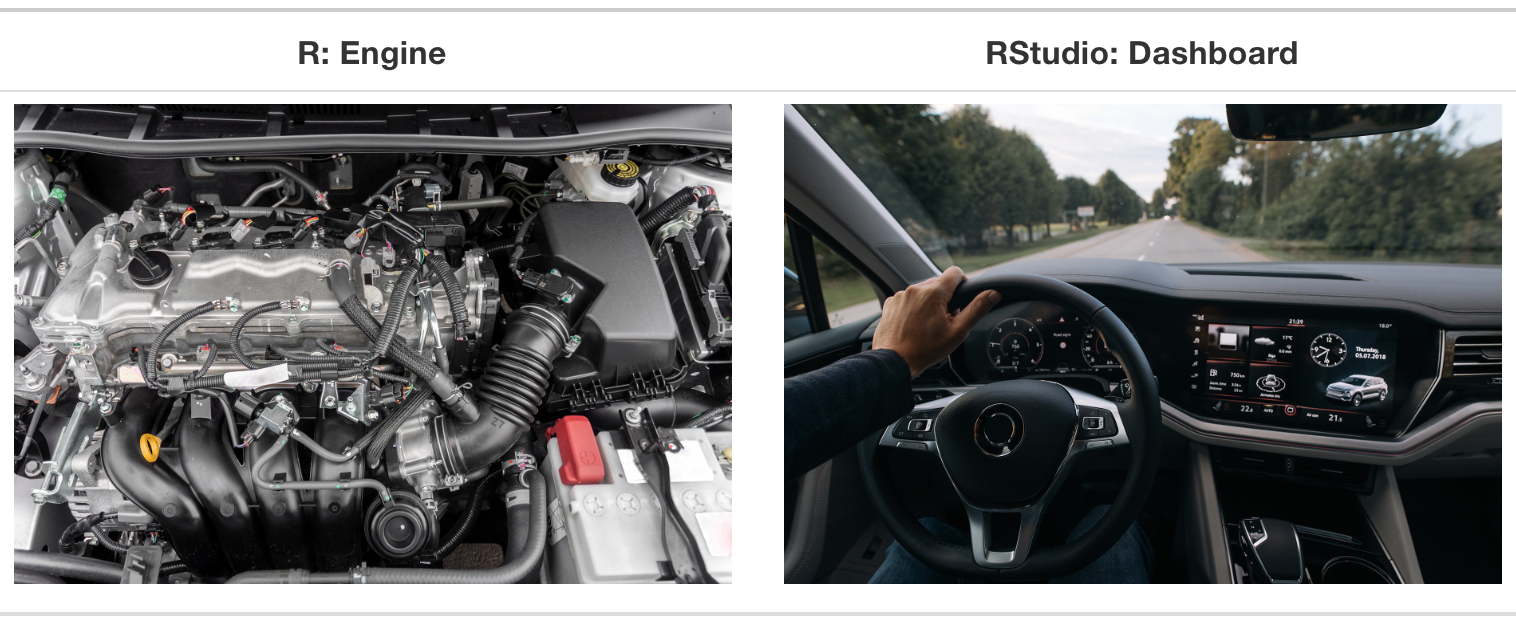
\includegraphics[width=0.95\linewidth]{fig/R_vs_RStudio_1} \caption{Analogy of difference between R and RStudio.}\label{fig:R-vs-RStudio-1}
\end{figure}

More precisely, R is a programming language that runs computations, while RStudio is an \emph{integrated development environment (IDE)} that provides an interface by adding many convenient features and tools. So just as the way of having access to a speedometer, rearview mirrors, and a navigation system makes driving much easier, using RStudio's interface makes using R much easier as well.

Much as we don't drive a car by interacting directly with the engine but rather by interacting with elements on the car's dashboard, we won't be using R directly but rather we will use RStudio's interface. After you install R and RStudio on your computer, you'll have two new \emph{programs} (also called \emph{applications}) you can open. We'll always work in RStudio and not in the R application. Figure \ref{fig:R-vs-RStudio-2a} shows what icon you should be clicking on your computer.

\begin{figure}

\includegraphics[width=0.9\linewidth]{fig/R_vs_RStudio} \caption{Icons of R versus RStudio on your computer.}\label{fig:R-vs-RStudio-2a}
\end{figure}

After you open RStudio, you should see something similar to Figure \ref{fig:RStudio-interfacea} where three or four panels dividing the screen.

\begin{figure}
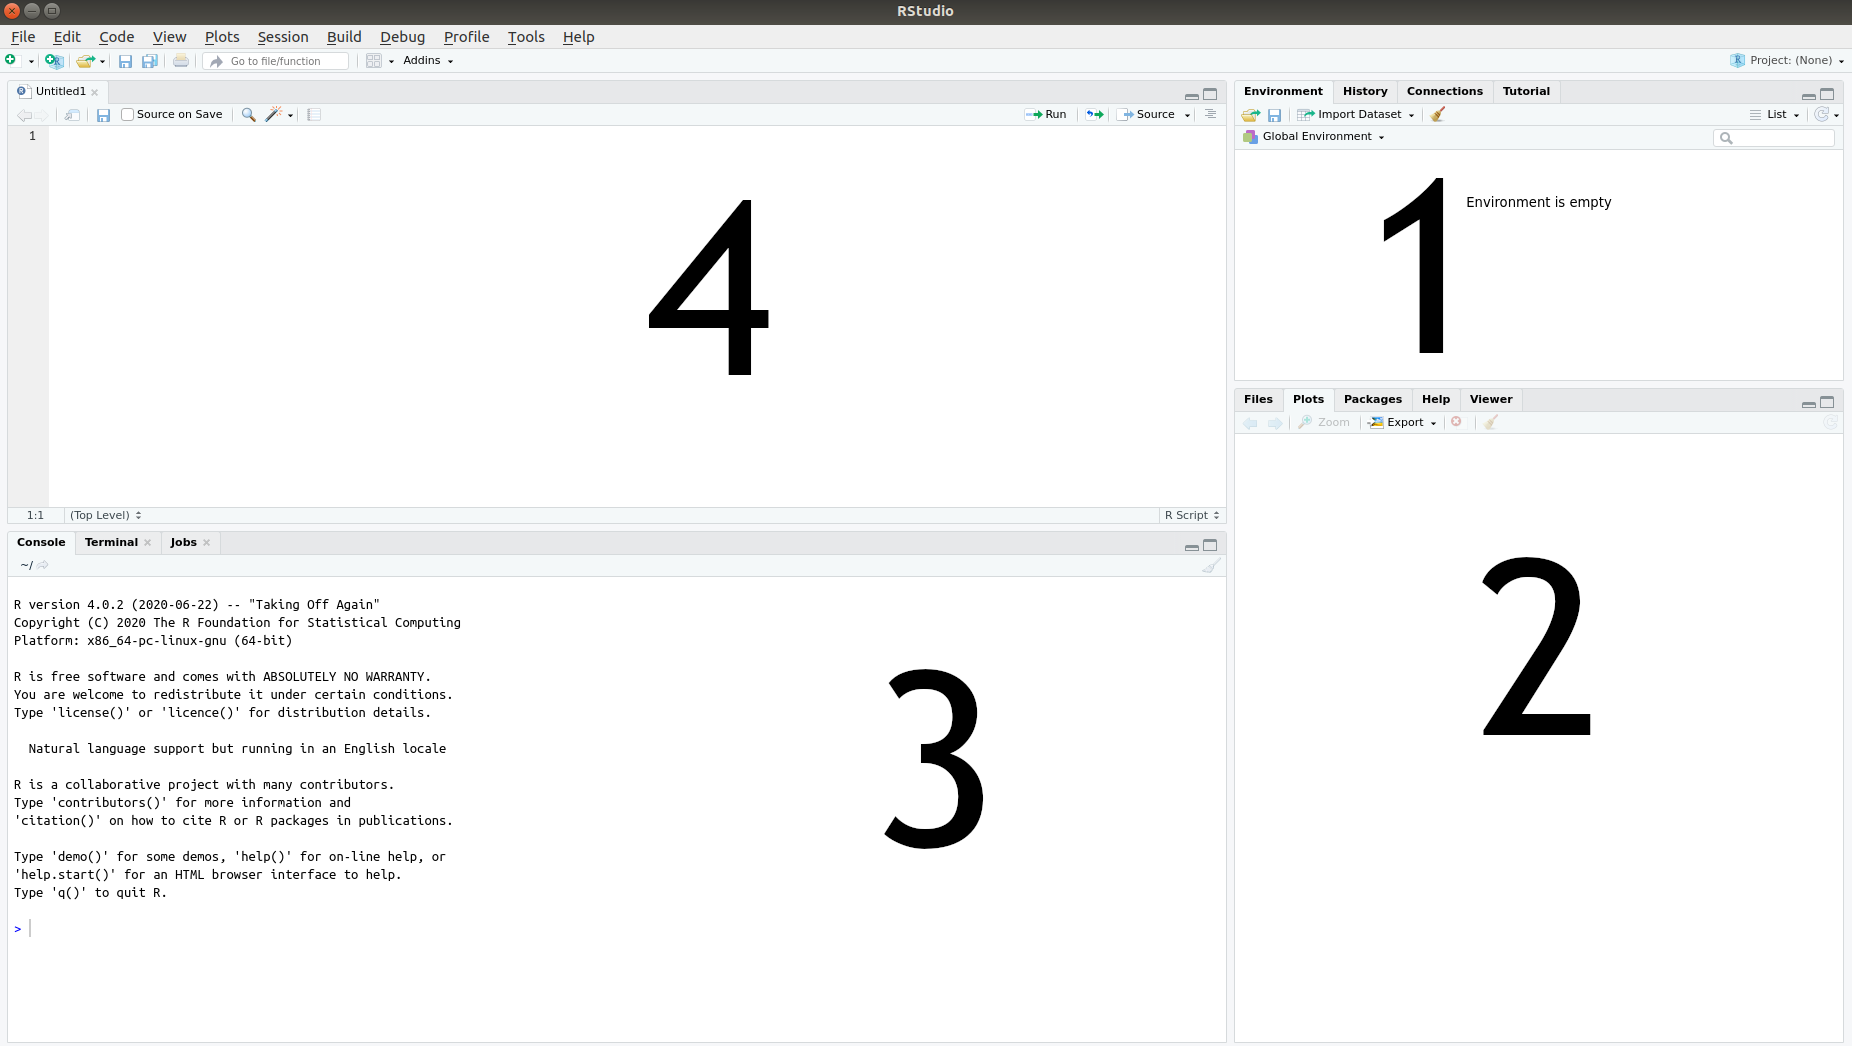
\includegraphics[width=0.93\linewidth]{fig/rstudio2} \caption{RStudio interface to R.}\label{fig:RStudio-interfacea}
\end{figure}

\begin{enumerate}
\def\labelenumi{\arabic{enumi}.}
\tightlist
\item
  The \emph{Environment} panel, where a list of the data you have imported and created can be found.
\item
  The \emph{Files}, \emph{Plots} and \emph{Help} panel, where you can see a list of available files, will be able to view graphs that you produce, and can find help documents for different parts of R.
\item
  The \emph{Console} panel, used for running code. This is where we'll start with the first few examples.
\item
  The \emph{Script} panel, used for writing code. This is where you'll spend most of your time working.
\end{enumerate}

The \emph{Console} panel will contain R's startup message, which shows information about which version of R you're running. My startup message at the time of writing was as follows:

\begin{quote}
R version 4.1.2 (2021-11-01) -- ``Bird Hippie''
Copyright (C) 2021 The R Foundation for Statistical Computing
Platform: x86\_64-pc-linux-gnu (64-bit)

R is free software and comes with ABSOLUTELY NO WARRANTY.
You are welcome to redistribute it under certain conditions.
Type `license()' or `licence()' for distribution details.

Natural language support but running in an English locale

R is a collaborative project with many contributors.
Type `contributors()' for more information and
`citation()' on how to cite R or R packages in publications.

Type `demo()' for some demos, `help()' for on-line help, or
`help.start()' for an HTML browser interface to help.
Type `q()' to quit R.
\end{quote}

If you don't have panel number 4, open it by opening an existing R-script or creating a new one. You can create a new on by clicking \emph{Ctrl+Shift+N} (alternatively, you can use the menu: File\(\rightarrow\)New File\(\rightarrow\)R Script).

You can resize the panels as you like, either by clicking and dragging their borders or using the minimise/maximise buttons in the upper right corner of each panel. Clicking \emph{Ctrl++} and \emph{Ctrl+-} allows to make the fonts larger or smaller.

When you exit RStudio, you will be asked if you wish to \emph{save your workspace}, meaning that the data that you've worked with will be stored so that it is available the next time you run R. That might sound like a good idea, but in general, I recommend that you don't save your workspace, as that often turns out to cause problems down the line. It is almost invariably a much better idea to simply rerun the code you worked with in your next R session.

\hypertarget{how-to-use-r-and-rstudio-without-installation}{%
\section{How to use R and RStudio without installation}\label{how-to-use-r-and-rstudio-without-installation}}

If you don't want to install R on your PC or you don't have admin rights to do so, you can use RStudio online doing \emph{cloud computing} on \url{https://posit.cloud/}.
Posit Cloud (formerly RStudio Cloud) is a cloud-based solution that allows anyone to do, share, teach and learn data science online. It is free for individuals with some restrictions and limited capacities.

\hypertarget{installing}{%
\section{Installing R and RStudio}\label{installing}}

You will first need to download and install both R and RStudio (Desktop version) on your computer. It is important that you install R first and then install RStudio.

\begin{enumerate}
\def\labelenumi{\arabic{enumi}.}
\tightlist
\item
  \textbf{Do this firstly:} Download and install R by going to \url{https://cloud.r-project.org/}. \index{R!installation}

  \begin{itemize}
  \tightlist
  \item
    If you are a Windows user: Click on ``Download R for Windows'', then click on ``base'', then click on the Download link.
  \item
    If you are macOS user: Click on ``Download R for (Mac) OS X'', then under ``Latest release:'' click on R-X.X.X.pkg, where R-X.X.X is the version number. For example, the latest version of R as of November 25, 2019 was R-3.6.1.
  \item
    If you are a Linux user: Click on ``Download R for Linux'' and choose your distribution for more information on installing R for your setup.
  \end{itemize}
\item
  \textbf{Do this secondly:} Download and install RStudio at \url{https://www.rstudio.com/products/rstudio/download/}.

  \begin{itemize}
  \tightlist
  \item
    Scroll down to ``Installers for Supported Platforms'' near the bottom of the page.
  \item
    Click on the download link corresponding to your computer's operating system.
  \end{itemize}
\end{enumerate}

\hypertarget{packages}{%
\section{What are R packages?}\label{packages}}

A package is basically just a big collection of functions, data sets and other R objects that are all grouped together under a common name. Some packages are already installed when you put R on your computer, but the vast majority of them of R packages are out there on the internet, waiting for you to download, install and use them.
R packages are collections of functions and data sets developed by the community. They increase the power of R by improving existing base R functionalities, or by adding new ones. For example, if you are usually working with data frames, probably you will have heard about \emph{dplyr} or \emph{data.table}, two of the most popular R packages. More than 10,000 packages are available at the official repository (CRAN) and many more are publicly available through the internet.

In this section, I'll describe how to work with packages using the Rstudio tools. Along the way, you'll see that whenever you get Rstudio to do something (e.g., install a package), you'll actually see the R commands that get created.

However, before we get started, there's a critical distinction that you need to understand, which is the difference between having a package \textbf{installed} on your computer, and having a package \textbf{loaded} in R. When you install R on your computer only a small number of packages come bundled with the basic R installation. The installed packages are on your computer. The critical thing to remember is that just because something is on your computer doesn't mean R can use it. In order for R to be able to \emph{use} one of your installed packages, that package must also be \emph{loaded}. Generally, when you open up R, only a few of these packages (about 7 or 8) are actually loaded. Basically what it boils down to is this:

\begin{enumerate}
\def\labelenumi{\arabic{enumi}.}
\tightlist
\item
  A package must be installed before it can be loaded.
\item
  A package must be loaded before it can be used.
\end{enumerate}

We only need to install a package once on our computer. However, to use the package, we need to load the library every time we start a new R environment. You can think of this as installing a bulb versus turning on the light.

\begin{figure}
\centering
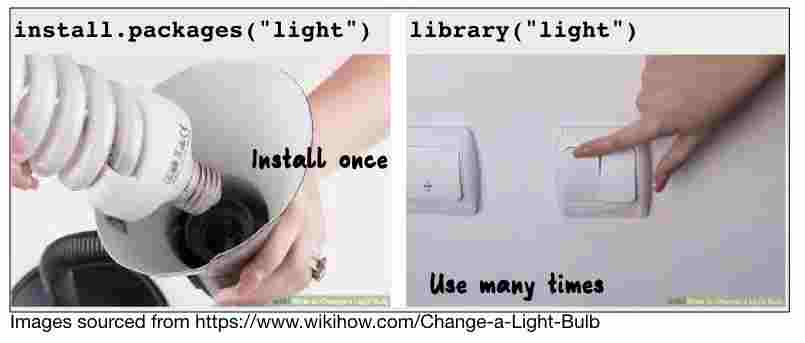
\includegraphics[width=0.5\textwidth,height=\textheight]{fig/lightpackage.jpeg}
\caption{\label{fig:lightpackage} Installing packages}
\end{figure}

The two step process might seem a little odd at first, but the designers of R had very good reasons to do it this way. That is, there are more than 10.000 packages, and probably about 8000 authors of packages, and no-one really knows what all of them do. Keeping the installation separate from the loading minimizes the chances that two packages will interact with each other in a nasty way. Moreover having installed all available packages would probably blow your hard disk.

Another good analogy for R packages \index{R packages} is they are like apps you can download onto a mobile phone:

\begin{figure}
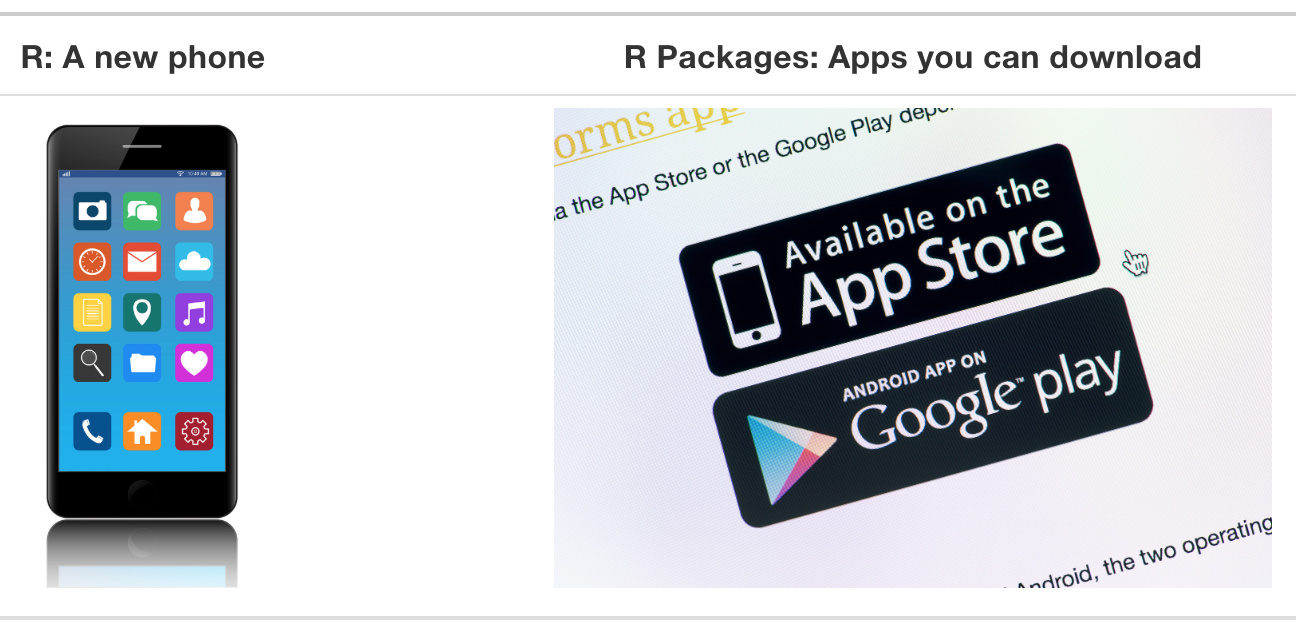
\includegraphics[width=0.7\linewidth]{fig/R_vs_R_packages} \caption{Analogy of R versus R packages.}\label{fig:R-vs-R-packages}
\end{figure}

So R is like a new mobile phone: while it has a certain amount of features when you use it for the first time, it doesn't have everything. R packages are like the apps you can download onto your phone from Apple's App Store or Android's Google Play.

\hypertarget{package-installation}{%
\subsection{Package installation}\label{package-installation}}

There are two ways to install an R package: an easy way and a very easy way. \index{R packages!installation} Let's install the \texttt{ggplot2} package the easy way first as shown in Figure \ref{fig:easy-way-install}. In the Files pane of RStudio:

\begin{enumerate}
\def\labelenumi{\alph{enumi})}
\tightlist
\item
  Click on the ``Packages'' tab.
\item
  Click on ``Install'' next to Update.
\item
  Type the name of the package under ``Packages (separate multiple with space or comma):'' In this case, type \texttt{ggplot2}.
\item
  Click ``Install.''
\end{enumerate}

\begin{figure}
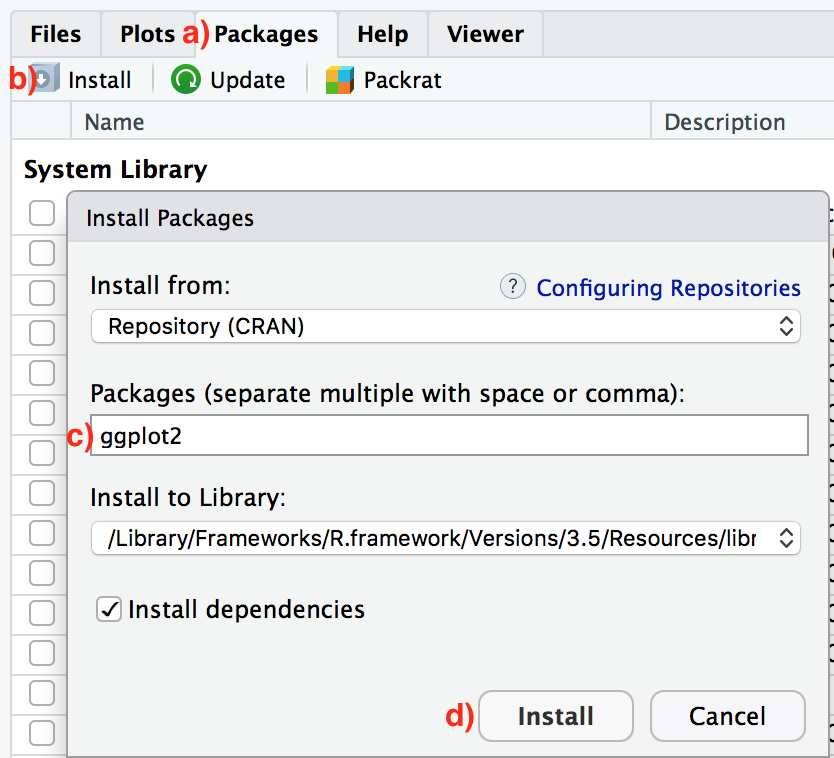
\includegraphics[width=0.55\linewidth,height=0.55\textheight]{fig/install_packages_easy_way} \caption{Installing packages in R the easy way.}\label{fig:easy-way-install}
\end{figure}

An alternative way to install a package is by typing

\begin{Shaded}
\begin{Highlighting}[]
\FunctionTok{install.packages}\NormalTok{(}\StringTok{"ggplot2"}\NormalTok{)}
\end{Highlighting}
\end{Shaded}

in the console pane of RStudio and pressing Return/Enter on your keyboard. Note you must include the quotation marks around the name of the package.

Much like an app on your phone, you only have to install a package once. However, if you want to update a previously installed package to a newer version, you need to re-install it by repeating the earlier steps or you use \texttt{update.packages()}. To uninstall packages you can use \texttt{remove.packages()}.

The installation of packages can take some time. However, if your CPU has many cores, you can speed up the process a lot using the argument \texttt{Ncpus} like this \texttt{update.packages(ask\ =\ F,\ Ncpus\ =\ 4L)}. This option allows you to adjust the number of parallel processes R can use on your PC. So, if you have a CPU with many cores you can increase that number.

\hypertarget{package-loading}{%
\subsection{Package loading}\label{package-loading}}

Recall that after you've installed a package, you need to \emph{load it}. In other words, you need to \emph{open it}. We do this by using the \texttt{library()} command. \index{R packages!loading}

For example, to load the \texttt{ggplot2} package, run the following code in the console pane. What do we mean by ``run the following code''? Either type or copy-and-paste the following code into the console pane and then hit the Enter key.

\begin{Shaded}
\begin{Highlighting}[]
\FunctionTok{library}\NormalTok{(}\StringTok{"ggplot2"}\NormalTok{)}
\end{Highlighting}
\end{Shaded}

If after running the earlier code, a blinking cursor returns next to the \texttt{\textgreater{}} ``prompt'' sign, it means you were successful and the \texttt{ggplot2} package is now loaded and ready to use. If, however, you get a red ``error message'' that reads

\begin{verbatim}
Error in library(ggplot2) : there is no package called ‘ggplot2’
\end{verbatim}

It means that you didn't successfully install it. If you get this error message, go back to section \ref{package-installation} on R package installation and make sure to install the \texttt{ggplot2} package before proceeding.

One very common mistake new R users make when wanting to use particular packages is they forget to \emph{load} them first by using the \texttt{library()} command we just saw. Remember: \emph{you have to load each package you want to use every time you start RStudio.} If you don't first \emph{load} a package, but attempt to use one of its features, you'll see an error message similar to:

\begin{verbatim}
Error: could not find function
\end{verbatim}

R is informing you that you are attempting to use a function from a package that has not yet been loaded. Forgetting to load packages is a common mistake made by new users, and it can be a bit frustrating to get used to at first. However, with practice, it will become second nature for you.
Unloading packages can be done with \texttt{detach(,\ unload=TRUE)}.

\hypertarget{what-is-a-function-in-r}{%
\section{What is a function in R?}\label{what-is-a-function-in-r}}

One of the keys to understand R is a \emph{functional programming language}. Or, to put in in the words of \citet[p.~4]{Chambers2017Extending}: ``Everything that happens is a function call.'' When you like to exit R, for example, you do it with the function \texttt{q()}:

\begin{Shaded}
\begin{Highlighting}[]
\NormalTok{\textgreater{} q()}
\NormalTok{Save workspace image? [y/n/c]: }
\end{Highlighting}
\end{Shaded}

If you don't want to be asked what you want to do with your workspace (that is the place where you store all your objects, see section \ref{sec:objects}) you can do it with an argument that is part of the function:

\begin{Shaded}
\begin{Highlighting}[]
\NormalTok{\textgreater{} q(save = "no")}
\end{Highlighting}
\end{Shaded}

\hypertarget{sec:objects}{%
\section{What are objects in R?}\label{sec:objects}}

Everything you do is made with a function and ``everything that exists in R is an object'' \citep[p.~4]{Chambers2017Extending}. Objects are the fundamental units that are used to store information. Objects can be created using a variety of data types, including vectors, matrices, data frames, lists, functions. All objects are shown in the \emph{workspace} which is shown in the \emph{Environment} panel.

In R, you can show the content of the workspace with \texttt{ls()}. The function \texttt{rm()} allows to remove objects and with \texttt{rm(list=ls())} you clear all objects from the workspace.

\hypertarget{are-there-some-guidelines-for-working-with-r}{%
\section{Are there some guidelines for working with R?}\label{are-there-some-guidelines-for-working-with-r}}

To avoid running into issues with R, it's important to be aware of the some conventions, rules, and best practices that apply to the language. While it can be tedious to go through all of the do's and don'ts in detail, following them can make your life with R much easier. Trust me, the benefits of adhering to these guidelines will become clear over time. Here is a non-exhaustive list:

\begin{enumerate}
\def\labelenumi{\arabic{enumi}.}
\tightlist
\item
  Do remember that R programming language is case sensitive.
\item
  Do start names of objects such as vectors, numbers, variables, and data frames with a letter, not a number.
\item
  Do avoid using dots in names of objects.
\item
  Do avoid using certain keywords in naming objects, such as if, else, repeat, while, function, for, in, next, break, TRUE, FALSE, NULL, Inf, NaN, and NA.
\item
  Do use front slash \texttt{/} instead of backslash \texttt{\textbackslash{}} for navigating the file system.
\item
  Do not use whitespace and indentation for naming files, directories, or objects.
\item
  Do not ignore warnings or errors unless you know what they mean.
\item
  Do define objects to represent hard-coded values instead of using them directly in code.
\item
  Do remember to (install and) load packages that contain functions you want to use.
\item
  Do remember to set your working directory. (Tip: Use R Studio projects, see \ref{sec:rstudioprojects})
\item
  Do remember to comment your code.
\item
  Do use \texttt{\textless{}-} instead of \texttt{=} for assignment.
\end{enumerate}

An exhaustive style guide on how to write code can be found here: \url{https://style.tidyverse.org}

\hypertarget{swirl}{%
\chapter{Learn interactively with swirl}\label{swirl}}

The R package \emph{swirl} makes it fun and easy to learn R programming and data science.
\emph{swirl} teaches you R programming and data science interactively, at your own pace,
and right in the R console! You get immediate feedback on your progress.
If you are new to R, have no fear. \emph{swirl} will walk you through each of the steps
required to employ Rstudio and R for your purpose.
To start it, please follow my instructions precisely!

Open Rstudio and type in the console the following:

\begin{Shaded}
\begin{Highlighting}[]
\FunctionTok{install.packages}\NormalTok{(}\StringTok{"swirl"}\NormalTok{)}
\FunctionTok{library}\NormalTok{(}\StringTok{"swirl"}\NormalTok{)}
\FunctionTok{install\_course\_github}\NormalTok{(}\StringTok{"hubchev"}\NormalTok{, }\StringTok{"swirl{-}it"}\NormalTok{)}
\FunctionTok{swirl}\NormalTok{()}
\end{Highlighting}
\end{Shaded}

The above lines of code do the following:

\begin{itemize}
\tightlist
\item
  Install the \emph{swirl} package.
\item
  Load the \emph{swirl} package.
\item
  Install my \emph{swirl} course that is hosted on GitHub.
\item
  With \emph{swirl} you start \emph{swirl} and your learning experience.
\end{itemize}

If the course has failed to install, you can try to download the file \texttt{swirl-it.swc} from \url{https://github.com/hubchev/swirl-it} and install the course with loading the swirl package and typing \texttt{install\_course()} into the console.

Please choose the course \emph{swirl-it} and the learning module \emph{huber-intro-1}.
You can exit \emph{swirl} at any time by typing \texttt{bye()} or by clicking the \emph{Esc} on your keyboard.

After you have successfully finished learning module \emph{huber-intro-1} please go ahead with the learning module \emph{huber-intro-2} that is also part of my swirl course \emph{swirl-it}.

\hypertarget{swirl-modules-on-data-analytical-basics}{%
\subsubsection*{\texorpdfstring{\emph{swirl} modules on data analytical basics}{swirl modules on data analytical basics}}\label{swirl-modules-on-data-analytical-basics}}

In my swirl modules \emph{huber-data-1}, \emph{huber-data-2}, and \emph{huber-data-3} I introduce some very basic statistical principles on how to analyse data.

\hypertarget{swirl-module-on-the-tidyverse-package}{%
\subsubsection*{\texorpdfstring{\emph{swirl} module on the \texttt{tidyverse} package}{swirl module on the tidyverse package}}\label{swirl-module-on-the-tidyverse-package}}

I compiled a short \emph{swirl} module to introduce the \emph{tidyverse} universe. This is a powerful collection of packages which I discuss later on. The learning module is also part of my \emph{swirl-it} course.

\hypertarget{other-swirl-modules}{%
\subsubsection*{\texorpdfstring{Other \emph{swirl} modules}{Other swirl modules}}\label{other-swirl-modules}}

You can also install some other courses. You find a list of courses here \url{http://swirlstats.com/scn/index.html} or here \url{https://github.com/swirldev/swirl_courses}.

I recommend this one as it gives a general overview on very basic principles of R:

\begin{Shaded}
\begin{Highlighting}[]
\FunctionTok{library}\NormalTok{(swirl)}
\FunctionTok{install\_course\_github}\NormalTok{(}\StringTok{"swirldev"}\NormalTok{, }\StringTok{"R\_Programming\_E"}\NormalTok{)}
\FunctionTok{swirl}\NormalTok{()}
\end{Highlighting}
\end{Shaded}

\hypertarget{work-with-r-scripts}{%
\chapter{Work with R scripts}\label{work-with-r-scripts}}

\hypertarget{r-scripts-why-they-are-useful}{%
\section{R Scripts: Why they are useful}\label{r-scripts-why-they-are-useful}}

Typing functions into the console to run code may seem simple, but this interactive style has limitations:

\begin{itemize}
\tightlist
\item
  Typing commands one at a time can be cumbersome and time-consuming.
\item
  It's hard to save your work effectively.
\item
  Going back to the beginning when you make a mistake is annoying.
\item
  You can't leave notes for yourself.
\item
  Reusing and adapting analyses can be difficult.
\item
  It's hard to do anything except the basics.
\item
  Sharing your work with others can be challenging.
\end{itemize}

That's where having a transcript of all the code, which can be re-run and edited at any time, becomes useful. An R script is precisely that - a plain text file that contains code and comments and this comes with advantages:

\begin{itemize}
\tightlist
\item
  Scripts provide a record of everything you did during your data analysis.
\item
  You can easily edit and re-run code in a script.
\item
  Scripts allow you to leave notes for yourself.
\item
  Scripts make it easy to reuse and adapt analyses.
\item
  Scripts allow you to do more complex analyses.
\item
  Scripts make it easy to share your work with others.
\end{itemize}

\hypertarget{generate-write-and-run-r-scripts}{%
\section{Generate, write, and run R scripts}\label{generate-write-and-run-r-scripts}}

To \textbf{generate a script} you can

\begin{enumerate}
\def\labelenumi{\arabic{enumi}.}
\tightlist
\item
  Go to the \emph{File} menu, select \emph{New File} and then choose \emph{R Script} or
\item
  Use the keyboard shortcut \emph{Ctrl+Shift+N} (Windows) or \emph{Cmd+Shift+N} (Mac) or
\item
  Type the following command in the Console:
\end{enumerate}

\begin{Shaded}
\begin{Highlighting}[]
\FunctionTok{file.create}\NormalTok{(}\StringTok{"hello.R"}\NormalTok{)}
\end{Highlighting}
\end{Shaded}

In the first two ways, a new R script window will open which can be edited and should be saved either by clicking on the \emph{File} menu and selecting \emph{Save}, clicking the disk icon, or by using the shortcut \emph{Ctrl+S} (Windows) or \emph{Cmd+S} (Mac).
If you go for the third way, you need to open it manually.

Regardless of your preferred way of generating a script, we can now start \textbf{writing} our first script:

\begin{Shaded}
\begin{Highlighting}[]
\FunctionTok{setwd}\NormalTok{(}\StringTok{"/home/sthu/Dropbox/hsf/23{-}ss/ds/"}\NormalTok{)}
\NormalTok{x }\OtherTok{\textless{}{-}} \StringTok{"hello world"}
\FunctionTok{print}\NormalTok{(x)}
\end{Highlighting}
\end{Shaded}

\begin{verbatim}
## [1] "hello world"
\end{verbatim}

Then save the script using the menus (File \textgreater{} Save) as hello.R.

The above lines of code do the following:

\begin{itemize}
\tightlist
\item
  \texttt{setwd()} allows to set the working directory. If you are not familiar with file systems, please read section \ref{sec:navigation} in the appendix.
\item
  With the assignment operator \texttt{\textless{}-} we create an object that stores the words ``hello world'' in an object entitled \texttt{x}. In the next section \ref{sec:assignmentoper} the assignment operator is further explained.
\item
  With the third input we print the content of the object \texttt{x}.
\end{itemize}

So how do we \textbf{run the script}? Assuming that the \texttt{hello.R} file has been saved to your working directory, then you can run the script using the following command:

\begin{Shaded}
\begin{Highlighting}[]
\FunctionTok{source}\NormalTok{( }\StringTok{"hello.R"}\NormalTok{ )}
\end{Highlighting}
\end{Shaded}

Suppose you saved the script in a sub-folder called \texttt{scripts} of your working directory, then you need to run the script using the following command:

\begin{Shaded}
\begin{Highlighting}[]
\FunctionTok{source}\NormalTok{(}\StringTok{"./scripts/hello.R"}\NormalTok{) }
\end{Highlighting}
\end{Shaded}

Just note that the dot, \texttt{.}, means the current folder.
Instead of using the \texttt{source} function, you can click on the \texttt{source} button in Rstudio.

With the character \texttt{\#} you can write a comment in a script and R will simply ignore everything that follows in that line onwards.

\hypertarget{sec:assignmentoper}{%
\section{\texorpdfstring{The assignment operator: \texttt{\textless{}-}}{The assignment operator: \textless-}}\label{sec:assignmentoper}}

Suppose I'm trying to calculate how much money I'm going to make from this book. I agree, it is an unrealistic example but it will help you to understand R.
Let's assume I'm only going to sell 350 copies. To create a variable called \texttt{sales} and assigns a value to it, we need to use the \emph{assignment operator} of R, which is \texttt{\textless{}-} as follows:

\begin{Shaded}
\begin{Highlighting}[]
\NormalTok{sales }\OtherTok{\textless{}{-}} \DecValTok{350}
\end{Highlighting}
\end{Shaded}

When you hit enter, R doesn't print out any output. If you are using Rstudio, and the \emph{environment panel} you can see that something happened there, can you? It just gives you another command prompt. However, behind the scenes R has created a variable called \texttt{sales} and given it a value of \texttt{350}. You can check that this has happened by asking R to print the variable on screen. And the simplest way to do that is to type the name of the variable and hit enter.

\begin{Shaded}
\begin{Highlighting}[]
\NormalTok{sales}
\end{Highlighting}
\end{Shaded}

\begin{verbatim}
## [1] 350
\end{verbatim}

Worth a mentioning is the curious features of R that there are several different ways of making assignments. In addition to the \texttt{\textless{}-} operator, we can also use \texttt{-\textgreater{}} and \texttt{=}. If you want to use \texttt{-\textgreater{}}, you might expect from just looking at the symbol you should write it like this:

\begin{Shaded}
\begin{Highlighting}[]
\DecValTok{350} \OtherTok{{-}\textgreater{}}\NormalTok{ sales}
\end{Highlighting}
\end{Shaded}

However, it is common practice to use \texttt{\textless{}-} and I recommend only to use this one because it is easier to read in scripts.

\hypertarget{doing-calculation-in-scripts}{%
\section{Doing calculation in scripts}\label{doing-calculation-in-scripts}}

R can do any kind of arithmetic calculation with the arithmetic operators given in the table below. Using the assignment operator, R functions, and the features of a R script is easy and gives an idea how R works and how you should embrace the power of the programming language.

\begin{longtable}[]{@{}lccc@{}}
\toprule\noalign{}
operation & operator & example input & example output \\
\midrule\noalign{}
\endhead
\bottomrule\noalign{}
\endlastfoot
addition & + & 10+2 & 12 \\
subtraction & - & 9-3 & 6 \\
multiplication & * & 5*5 & 25 \\
division & / & 10/3 & 3 \\
power & \texttt{\^{}} & 5\^{}2 & 25 \\
\end{longtable}

So please copy and past the following lines of code into a R script of yours, try to run it on your PC, and try to understand it. Of course, you have to tweak the script a bit to make it run on your PC. For example, I doubt you have the same working directory that I decided to use.

\begin{Shaded}
\begin{Highlighting}[]
\CommentTok{\# Set working directory}
\FunctionTok{setwd}\NormalTok{(}\StringTok{"\textasciitilde{}/Dropbox/hsf/23{-}ss/ds"}\NormalTok{)}
\CommentTok{\# Create a vector that contains the sales data}
\NormalTok{sales\_by\_month }\OtherTok{\textless{}{-}} \FunctionTok{c}\NormalTok{(}\DecValTok{0}\NormalTok{, }\DecValTok{100}\NormalTok{, }\DecValTok{200}\NormalTok{, }\DecValTok{50}\NormalTok{, }\DecValTok{3}\NormalTok{, }\DecValTok{4}\NormalTok{, }\DecValTok{8}\NormalTok{, }\DecValTok{0}\NormalTok{, }\DecValTok{0}\NormalTok{, }\DecValTok{0}\NormalTok{, }\DecValTok{0}\NormalTok{, }\DecValTok{0}\NormalTok{)}
\NormalTok{sales\_by\_month}
\NormalTok{sales\_by\_month[}\DecValTok{2}\NormalTok{]}
\NormalTok{sales\_by\_month[}\DecValTok{4}\NormalTok{]}
\NormalTok{february\_sales }\OtherTok{\textless{}{-}}\NormalTok{ sales\_by\_month[}\DecValTok{2}\NormalTok{]}
\NormalTok{february\_sales}
\NormalTok{sales\_by\_month[}\DecValTok{5}\NormalTok{] }\OtherTok{\textless{}{-}} \DecValTok{25} \CommentTok{\# added May sales data}
\NormalTok{sales\_by\_month}
\CommentTok{\# Do I have 12 month?}
\FunctionTok{length}\NormalTok{( }\AttributeTok{x =}\NormalTok{ sales\_by\_month )}
\CommentTok{\# Assume each unit costs 7 Euro, then the revenue is}
\NormalTok{price }\OtherTok{\textless{}{-}} \DecValTok{7}
\NormalTok{revenue }\OtherTok{\textless{}{-}}\NormalTok{ sales\_by\_month}\SpecialCharTok{*}\NormalTok{price}
\NormalTok{revenue}
\CommentTok{\# To get statistics for daily revenue we define the number of days:}
\NormalTok{days\_per\_month }\OtherTok{\textless{}{-}} \FunctionTok{c}\NormalTok{(}\DecValTok{31}\NormalTok{, }\DecValTok{28}\NormalTok{, }\DecValTok{31}\NormalTok{, }\DecValTok{30}\NormalTok{, }\DecValTok{31}\NormalTok{, }\DecValTok{30}\NormalTok{, }\DecValTok{31}\NormalTok{, }\DecValTok{31}\NormalTok{, }\DecValTok{30}\NormalTok{, }\DecValTok{31}\NormalTok{, }\DecValTok{30}\NormalTok{, }\DecValTok{31}\NormalTok{)}
\CommentTok{\# Calculate the daily revenue}
\NormalTok{revenue\_per\_day }\OtherTok{\textless{}{-}}\NormalTok{ revenue}\SpecialCharTok{/}\NormalTok{days\_per\_month}
\NormalTok{revenue\_per\_day }
\CommentTok{\# round number }
\FunctionTok{round}\NormalTok{(revenue\_per\_day) }
\end{Highlighting}
\end{Shaded}

Use the ``\texttt{?}'' to search for the documentation of all functions used. In particular, do you understand how the function \texttt{round()} works? What arguments does the function contain? How can you manipulate the pre-defined arguments. For example, can you calculate the rounded revenue per day with two or four digits? Try it out!

\begin{Shaded}
\begin{Highlighting}[]
\NormalTok{?}\FunctionTok{round}\NormalTok{()}
\end{Highlighting}
\end{Shaded}

\hypertarget{sec:generics}{%
\section{User-defined functions}\label{sec:generics}}

One of the great strengths of R is the user's ability to add functions. Sometimes there is a small task (or series of tasks) you need done and you find yourself having to repeat it multiple times. In these types of situations it can be helpful to create your own custom function. The structure of a function is given below:

\begin{Shaded}
\begin{Highlighting}[]
\NormalTok{name\_of\_function }\OtherTok{\textless{}{-}} \ControlFlowTok{function}\NormalTok{(argument1, argument2) \{}
\NormalTok{    statements or code that does something}
    \FunctionTok{return}\NormalTok{(something)}
\NormalTok{\}}
\end{Highlighting}
\end{Shaded}

First you give your function a name.
Then you assign value to it, where the value is the function.
When defining the function you will want to provide the list of arguments required (inputs and/or options to modify behavior of the function), and wrapped between curly brackets place the tasks that are being executed on/using those arguments. The argument(s) can be any type of object (like a scalar, a matrix, a dataframe, a vector, a logical, etc), and it's not necessary to define what it is in any way.
Finally, you can return the value of the object from the function, meaning pass the value of it into the global environment. The important idea behind functions is that objects that are created within the function are local to the environment of the function -- they don't exist outside of the function. Note, a function doesn't require any arguments.

Let's try creating a simple example function. This function will take in a numeric value as input, and return the squared value.

\begin{Shaded}
\begin{Highlighting}[]
\NormalTok{square\_it }\OtherTok{\textless{}{-}} \ControlFlowTok{function}\NormalTok{(x) \{ }
\NormalTok{   square }\OtherTok{\textless{}{-}}\NormalTok{ x }\SpecialCharTok{*}\NormalTok{ x}
   \FunctionTok{return}\NormalTok{(square)}
\NormalTok{\} }
\end{Highlighting}
\end{Shaded}

Now, we can use the function as we would any other function. We type out the name of the function, and inside the parentheses we provide a numeric value \texttt{x}:

\begin{Shaded}
\begin{Highlighting}[]
\FunctionTok{square\_it}\NormalTok{(}\DecValTok{5}\NormalTok{)}
\end{Highlighting}
\end{Shaded}

\begin{verbatim}
## [1] 25
\end{verbatim}

Let us get back to script with sales and try to calculate the monthly growth rates of revenue using a self-written function.

The formula of a growth rate is clear:

\[ g=\left(\frac{y_t-y_{t-1}}{y_{t-1}}\right)\cdot 100=\left(\frac{y_t}{y_{t-1}}-1\right)\cdot 100 \]

So the challenge is to divide the value of \texttt{revenue} with the value of the previous period, a.k.a. the lagged value. Let us assume that the function \texttt{lag()} can give you exactly that value of a vector. Lets try it out:

\begin{Shaded}
\begin{Highlighting}[]
\FunctionTok{lag}\NormalTok{(revenue)}
\end{Highlighting}
\end{Shaded}

\begin{verbatim}
##  [1]    0  700 1400  350  175   28   56    0    0    0    0    0
## attr(,"tsp")
## [1]  0 11  1
\end{verbatim}

\begin{Shaded}
\begin{Highlighting}[]
\NormalTok{(revenue}\SpecialCharTok{/}\FunctionTok{lag}\NormalTok{(revenue)}\SpecialCharTok{{-}}\DecValTok{1}\NormalTok{)}\SpecialCharTok{*}\DecValTok{100} 
\end{Highlighting}
\end{Shaded}

\begin{verbatim}
##  [1] NaN   0   0   0   0   0   0 NaN NaN NaN NaN NaN
## attr(,"tsp")
## [1]  0 11  1
\end{verbatim}

Unfortunately, this does not work out. The \texttt{lag()} function does not work as we think it should. Well, the reason is simply that we are using the wrong function. The current \texttt{lag()} function is part of the stats package which is part of the package \texttt{stats} which is part of R base and is loaded automatically. The \texttt{lag()} function we aim to use stems from the dplyr package which we must install and load to be able to use it. So let's do it:

\begin{Shaded}
\begin{Highlighting}[]
\CommentTok{\# check if the package is installed}
\FunctionTok{find.package}\NormalTok{(}\StringTok{"dplyr"}\NormalTok{)}
\end{Highlighting}
\end{Shaded}

\begin{verbatim}
## [1] "/usr/local/lib/R/site-library/dplyr"
\end{verbatim}

\begin{Shaded}
\begin{Highlighting}[]
\CommentTok{\# I already installed the package so I can just load it}
\CommentTok{\# install.packages("dplyr")}
\FunctionTok{library}\NormalTok{(}\StringTok{"dplyr"}\NormalTok{)}
\end{Highlighting}
\end{Shaded}

\begin{verbatim}
## 
## Attaching package: 'dplyr'
\end{verbatim}

\begin{verbatim}
## The following objects are masked from 'package:stats':
## 
##     filter, lag
\end{verbatim}

\begin{verbatim}
## The following objects are masked from 'package:base':
## 
##     intersect, setdiff, setequal, union
\end{verbatim}

This message informs us that among other functions the \texttt{lag()} function is \emph{masked}. That means that now the function of the newly loaded package is active. So, let's try again:

\begin{Shaded}
\begin{Highlighting}[]
\FunctionTok{lag}\NormalTok{(revenue)}
\end{Highlighting}
\end{Shaded}

\begin{verbatim}
##  [1]   NA    0  700 1400  350  175   28   56    0    0    0    0
\end{verbatim}

\begin{Shaded}
\begin{Highlighting}[]
\NormalTok{(revenue}\SpecialCharTok{/}\FunctionTok{lag}\NormalTok{(revenue)}\SpecialCharTok{{-}}\DecValTok{1}\NormalTok{)}\SpecialCharTok{*}\DecValTok{100} 
\end{Highlighting}
\end{Shaded}

\begin{verbatim}
##  [1]   NA  Inf  100  -75  -50  -84  100 -100  NaN  NaN  NaN  NaN
\end{verbatim}

That looks good now. And here is a way to calculate growth rates with a self-written function:

\begin{Shaded}
\begin{Highlighting}[]
\NormalTok{growth\_rate }\OtherTok{\textless{}{-}} \ControlFlowTok{function}\NormalTok{(x)(x}\SpecialCharTok{/}\FunctionTok{lag}\NormalTok{(x)}\SpecialCharTok{{-}}\DecValTok{1}\NormalTok{)}\SpecialCharTok{*}\DecValTok{100} 
\FunctionTok{growth\_rate}\NormalTok{(revenue)}
\end{Highlighting}
\end{Shaded}

\begin{verbatim}
##  [1]   NA  Inf  100  -75  -50  -84  100 -100  NaN  NaN  NaN  NaN
\end{verbatim}

\begin{Shaded}
\begin{Highlighting}[]
\NormalTok{sales\_gr\_rate }\OtherTok{\textless{}{-}} \FunctionTok{growth\_rate}\NormalTok{(revenue)}
\NormalTok{sales\_gr\_rate}
\end{Highlighting}
\end{Shaded}

\begin{verbatim}
##  [1]   NA  Inf  100  -75  -50  -84  100 -100  NaN  NaN  NaN  NaN
\end{verbatim}

In R, all functions are written by users, and it is not uncommon for two people to name their functions identically. In such cases, we must resolve the conflict by choosing which function to use. To use the lag function from the \texttt{stats} package, you can use the double colon operator \texttt{::} like this \texttt{stats::lag(arguments)}.

\begin{exercise}
\protect\hypertarget{exr:growthrate}{}\label{exr:growthrate}All roads lead to R(ome)

If you ask ten programmers to solve a particular problem, you will probably receive ten different soltuions that are all valid. R is no exception here. This can be very confussing when just started to learn R.

Below you find more ways to calculate the a growth rate. Do you understand them?

\begin{Shaded}
\begin{Highlighting}[]
\FunctionTok{c}\NormalTok{(}\ConstantTok{NA}\NormalTok{, }\FunctionTok{diff}\NormalTok{(revenue)}\SpecialCharTok{/}\FunctionTok{head}\NormalTok{(revenue, }\SpecialCharTok{{-}}\DecValTok{1}\NormalTok{))}\SpecialCharTok{*}\DecValTok{100}        
\end{Highlighting}
\end{Shaded}

\begin{verbatim}
##  [1]   NA  Inf  100  -75  -50  -84  100 -100  NaN  NaN  NaN  NaN
\end{verbatim}

\begin{Shaded}
\begin{Highlighting}[]
\NormalTok{(revenue}\SpecialCharTok{/}\FunctionTok{c}\NormalTok{(}\ConstantTok{NA}\NormalTok{,revenue[}\SpecialCharTok{{-}}\FunctionTok{length}\NormalTok{(revenue)])}\SpecialCharTok{{-}}\DecValTok{1}\NormalTok{)}\SpecialCharTok{*}\DecValTok{100}
\end{Highlighting}
\end{Shaded}

\begin{verbatim}
##  [1]   NA  Inf  100  -75  -50  -84  100 -100  NaN  NaN  NaN  NaN
\end{verbatim}

An often-used method for approximating growth rates is to calculate the differences in the logarithm of values over time. Section \ref{pipeoperator} illustrates how to perform this calculation with R.
\end{exercise}

\hypertarget{visualizing-data}{%
\chapter{Visualizing data}\label{visualizing-data}}

Data visualization is an art. The purposes of visualizing data are manifold. You can emphasize facts, get known to data, detect anomalies, and communicate a large amount of infirmation simply and intuitive. Whatever your goal is, thousand of appropiate ways exist to visualize data. Many decisions to take are simply a matter of taste. However, there are some conventions and guidelines that help you to make on average better decisions when designing a visualization:

\begin{itemize}
\tightlist
\item
  Good graphs are easy to understand and eye catching.
\item
  Graphs can be misleading and manipulative and that is opposing to the ideas of science. Thus, be responsible and honest.
\item
  Minimize colors and other attention-grabbing elements that are not directly related to the data of interest. Worldwide, there are approximately 300 million color blind people. In particular, red, green or blue light are problematic to color blind people. Thus, better rely on color schemes that are designed for colorblind people.
\item
  Don't truncate an axis or change the scaling within an axis just to make you your story more appealing. Show the full scale of the graph, then zoom to show the data of interest, if necessary.
\item
  Label and describe your chart sufficiently so that everybody can fully understand the content of the shown data set and statistics without having to study the notes of the graph for too long.
\item
  Don't do pie charts. They may look simple, but they're tricky to get right and there are usually better alternatives. Humans are not very good at comparing the size of angles and as there's no scale in pie plots, reading accurate values is difficult. Figure \ref{fig:piebad} may proof this.
\item
  For more tips, see:

  \begin{itemize}
  \tightlist
  \item
    \href{https://guides.library.duke.edu/datavis/topten}{Data Visualization: Chart Dos and Don'ts (by Duke University)}
  \end{itemize}
\item
  \href{https://www.kirchkamp.de/graph/}{Graphs and Visualising Data} by Oliver Kirchkamp. In particular, I highly recommend his \href{https://www.kirchkamp.de/oekonometrie/pdf/gra-p.pdf}{handout} \citep{Kirchkamp2018Using}. It discusses many pitfalls of visualizing data, instructs how to do good graphs, and he shows the corresponding R code of all graphs.\\
\item
  The \href{https://www.r-graph-gallery.com}{R Graph Gallery} offers shows graphs and the corresponding R code to replicate the graphs
\item
  The work of \href{www.edwardtufte.com}{Edward Tufte} and his book \emph{The Visual Display of Quantitative Information} \citep{Tufte2022Visual} are classical readings.
\end{itemize}

\begin{figure}
\centering
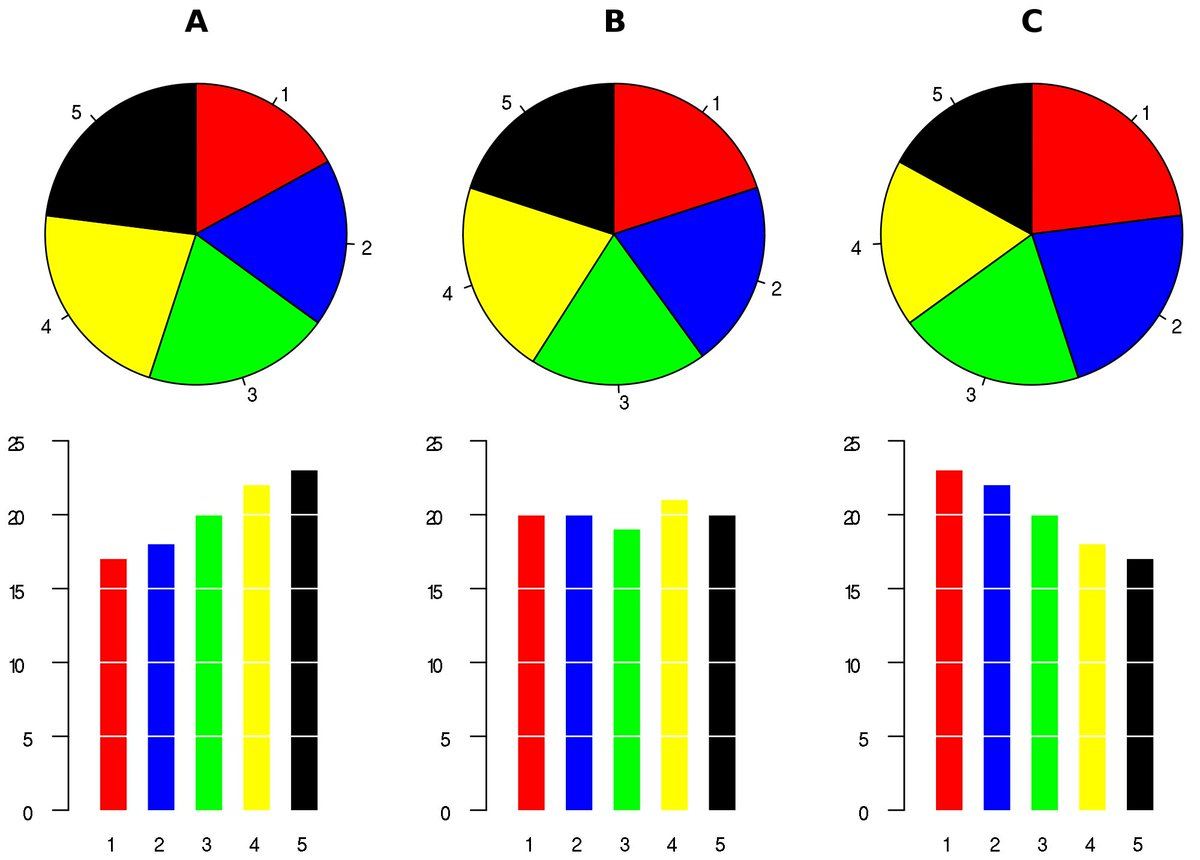
\includegraphics[width=0.7\textwidth,height=\textheight]{fig/piebad.jpeg}
\caption[\label{fig:piebad} Pie charts are problematic]{\label{fig:piebad} Pie charts are problematic\footnotemark{}}
\end{figure}
\footnotetext{Picture is taken from \url{https://en.wikipedia.org/wiki/Pie_chart}}

When it comes to data visualization, there's no better resource than the book by \citet{Wickham2023R}. It introduces the ggplot function which is part of the ggplot2 package which, in turn, is part of the tidyverse package. Thus, if you've installed and loaded tidyverse, you automatically have access to ggplot. Creating beautiful and informative graphs is easy with ggplot. To proof that claim, study section 2 (\href{https://r4ds.hadley.nz/data-visualize.html}{Data visualization}) of \citet{Wickham2023R}. To reap the best benefits from studying, I recommend to copy all the code that is shown in the book into a R script and try to run it on your PC. That is the best way to learn, understand, and create your own notes that may guide you later on. Whenever you see interesting code somewhere, try to run it on your PC. Moreover, I recommend the exercises of the book, they are challenging sometimes but to really understand code you need to run code yourself.

\hypertarget{manage-data}{%
\chapter{Manage data}\label{manage-data}}

\hypertarget{the-tidyverse-universe}{%
\section{The tidyverse universe}\label{the-tidyverse-universe}}

\begin{figure}
\centering

\includegraphics[width=0.3\textwidth,height=\textheight]{fig/tidyverse-logo.png}
\caption{\label{fig:tidyverse-logo} The tidyverse universe}
\end{figure}

The R package \emph{tidyverse} is a collection of R packages. All packages share an underlying design philosophy, grammar, and data structures.
The most popular packages are \emph{ggplot2}, \emph{dplyr}, \emph{tidyr}, \emph{readr}, \emph{purrr}, \emph{tibble}, \emph{stringr}, and \emph{forcats}. They provide functionality to model, transform, and visualize data. Tidyverse is extremely popular and many individual packages of tidyverse are regularly in the top 10 most downloaded R packages on CRAN\footnote{CRAN is a network of ftp and web servers around the world that store identical, up-to-date, versions of code and documentation for R, see: \url{https://cran.r-project.org}.}. How to do data science with tidyverse is the subject of multiple books and tutorials. In particular, the popular book \emph{R for Data Science} by \citet{Wickham2023R} is all about the tidyverse universe. Thus, I highly recommend reading sections 3 (\href{https://r4ds.hadley.nz/workflow-basics.html}{Workflow: basics}), 4 (\href{https://r4ds.hadley.nz/data-transform.html}{Data transformation}), and 6 (\href{https://r4ds.hadley.nz/data-tidy}{Data tidying}) of \citet{Wickham2023R}. Additionally, visit www.tidyverse.org and, if you still haven't done so, do the tidyverse module of my swirl package, called \emph{swirl-it}, see section \ref{swirl}.

To install and load tidyverse run the following lines of code:

\begin{Shaded}
\begin{Highlighting}[]
\FunctionTok{install.packages}\NormalTok{(}\StringTok{"tidyverse"}\NormalTok{)}
\FunctionTok{library}\NormalTok{(}\StringTok{"tidyverse"}\NormalTok{)}
\end{Highlighting}
\end{Shaded}

\hypertarget{pipeoperator}{%
\section{The pipe operator}\label{pipeoperator}}

The pipe operator, \%\textgreater\%, comes from the \emph{magrittr} package, which is also part of the tidyverse package. The pipe operator, \textbar\textgreater, has been part of base R since version 4.1.0. For most cases, these two operators are identical. The pipe operator is designed to help you write code in a way that is easier to read and understand. As R is a functional language, code often contains a lot of parentheses, ( and ). Nesting these parentheses together can be complex and make your R code hard to read and understand, which is where \textbar\textgreater{} comes to the rescue! It allows you to use the output of a function as the input of the next function. Consider the following example of code to explain the usage of the pipe operator:

\begin{Shaded}
\begin{Highlighting}[]
\CommentTok{\# create some data \textasciigrave{}x\textasciigrave{}}
\NormalTok{x }\OtherTok{\textless{}{-}} \FunctionTok{c}\NormalTok{(}\DecValTok{1}\NormalTok{, }\FloatTok{1.002}\NormalTok{, }\FloatTok{1.004}\NormalTok{, .}\DecValTok{99}\NormalTok{, .}\DecValTok{99}\NormalTok{)}
\CommentTok{\# take the logarithm of \textasciigrave{}x\textasciigrave{}, }
\NormalTok{log\_x }\OtherTok{\textless{}{-}} \FunctionTok{log}\NormalTok{(x)}
\CommentTok{\# compute the lagged and iterated differences (see \textasciigrave{}diff()\textasciigrave{})}
\NormalTok{growth\_rate\_x }\OtherTok{\textless{}{-}} \FunctionTok{diff}\NormalTok{(log\_x)}
\NormalTok{growth\_rate\_x}
\end{Highlighting}
\end{Shaded}

\begin{verbatim}
## [1]  0.001998003  0.001994019 -0.014042357  0.000000000
\end{verbatim}

\begin{Shaded}
\begin{Highlighting}[]
\CommentTok{\# round the result (4 digit)}
\NormalTok{growth\_rate\_x\_round }\OtherTok{\textless{}{-}} \FunctionTok{round}\NormalTok{(growth\_rate\_x, }\DecValTok{4}\NormalTok{)}
\NormalTok{growth\_rate\_x\_round }
\end{Highlighting}
\end{Shaded}

\begin{verbatim}
## [1]  0.002  0.002 -0.014  0.000
\end{verbatim}

That is rather long and we actually don't need objects log\_x, growth\_rate\_x, and growth\_rate\_x\_round.
Well, then let us write that in a nested function:

\begin{Shaded}
\begin{Highlighting}[]
\FunctionTok{round}\NormalTok{(}\FunctionTok{diff}\NormalTok{(}\FunctionTok{log}\NormalTok{(x)), }\DecValTok{4}\NormalTok{)}
\end{Highlighting}
\end{Shaded}

\begin{verbatim}
## [1]  0.002  0.002 -0.014  0.000
\end{verbatim}

This is short but hard to read and understand. The solution is the \emph{pipe}:

\begin{Shaded}
\begin{Highlighting}[]
\CommentTok{\# load one of these packages: \textasciigrave{}magrittr\textasciigrave{} or \textasciigrave{}tidyverse\textasciigrave{}}
\FunctionTok{library}\NormalTok{(tidyverse)}

\CommentTok{\# Perform the same computations on \textasciigrave{}x\textasciigrave{} as above}
\NormalTok{x }\SpecialCharTok{|\textgreater{}} 
  \FunctionTok{log}\NormalTok{() }\SpecialCharTok{|\textgreater{}}
  \FunctionTok{diff}\NormalTok{() }\SpecialCharTok{|\textgreater{}}
  \FunctionTok{round}\NormalTok{(}\DecValTok{4}\NormalTok{)}
\end{Highlighting}
\end{Shaded}

\begin{verbatim}
## [1]  0.002  0.002 -0.014  0.000
\end{verbatim}

You can read the \textbar\textgreater{} with \emph{``and then''} because it takes the results of some function \emph{``and then''} does something with that in the next.
For example, reading out loud the following code would sound something like this:

\begin{itemize}
\tightlist
\item
  I take the mtcars data, \emph{and then}
\item
  I consider only cars with more than 4 cylinders, \emph{and then}
\item
  I group the cars by the number of cylinders the cars have, \emph{and then}
\item
  I summarize the data and show the means of miles per gallon (mpg) and horse powers (hp) by groups of cars that distinguish by their number of cylinders.
\end{itemize}

\begin{Shaded}
\begin{Highlighting}[]
\NormalTok{mtcars }\SpecialCharTok{|\textgreater{}} 
  \FunctionTok{filter}\NormalTok{(cyl}\SpecialCharTok{\textgreater{}}\DecValTok{4}\NormalTok{) }\SpecialCharTok{|\textgreater{}} 
  \FunctionTok{group\_by}\NormalTok{(cyl) }\SpecialCharTok{|\textgreater{}} 
  \FunctionTok{summarise\_at}\NormalTok{(}\FunctionTok{c}\NormalTok{(}\StringTok{"mpg"}\NormalTok{, }\StringTok{"hp"}\NormalTok{), mean)}
\end{Highlighting}
\end{Shaded}

\begin{verbatim}
## # A tibble: 2 x 3
##     cyl   mpg    hp
##   <dbl> <dbl> <dbl>
## 1     6  19.7  122.
## 2     8  15.1  209.
\end{verbatim}

\hypertarget{import-data}{%
\section{Import data}\label{import-data}}

\hypertarget{vectors-and-matrices}{%
\subsection{Vectors and matrices}\label{vectors-and-matrices}}

We already got known to the c() function which allows to combine multiple values into a vector or list. Here are some examples how you can use this function to create vectors and matrices:

\begin{Shaded}
\begin{Highlighting}[]
\CommentTok{\# defining multiple vectors using the colon operator \textasciigrave{}:\textasciigrave{}}
\NormalTok{v\_a }\OtherTok{\textless{}{-}} \FunctionTok{c}\NormalTok{(}\DecValTok{1}\SpecialCharTok{:}\DecValTok{3}\NormalTok{)}
\NormalTok{v\_a}
\end{Highlighting}
\end{Shaded}

\begin{verbatim}
## [1] 1 2 3
\end{verbatim}

\begin{Shaded}
\begin{Highlighting}[]
\NormalTok{v\_b }\OtherTok{\textless{}{-}} \FunctionTok{c}\NormalTok{(}\DecValTok{10}\SpecialCharTok{:}\DecValTok{12}\NormalTok{)}
\NormalTok{v\_b}
\end{Highlighting}
\end{Shaded}

\begin{verbatim}
## [1] 10 11 12
\end{verbatim}

\begin{Shaded}
\begin{Highlighting}[]
\CommentTok{\# creating matrix}
\NormalTok{m\_ab }\OtherTok{\textless{}{-}} \FunctionTok{matrix}\NormalTok{(}\FunctionTok{c}\NormalTok{(v\_a, v\_b), }\AttributeTok{ncol =} \DecValTok{2}\NormalTok{)}
\NormalTok{m\_cbind }\OtherTok{\textless{}{-}} \FunctionTok{cbind}\NormalTok{(v\_a, v\_b)}
\NormalTok{m\_rbind }\OtherTok{\textless{}{-}} \FunctionTok{rbind}\NormalTok{(v\_a, v\_b)}

\CommentTok{\# print matrix}
\FunctionTok{print}\NormalTok{(m\_ab)}
\end{Highlighting}
\end{Shaded}

\begin{verbatim}
##      [,1] [,2]
## [1,]    1   10
## [2,]    2   11
## [3,]    3   12
\end{verbatim}

\begin{Shaded}
\begin{Highlighting}[]
\FunctionTok{print}\NormalTok{(m\_cbind)}
\end{Highlighting}
\end{Shaded}

\begin{verbatim}
##      v_a v_b
## [1,]   1  10
## [2,]   2  11
## [3,]   3  12
\end{verbatim}

\begin{Shaded}
\begin{Highlighting}[]
\FunctionTok{print}\NormalTok{(m\_rbind)}
\end{Highlighting}
\end{Shaded}

\begin{verbatim}
##     [,1] [,2] [,3]
## v_a    1    2    3
## v_b   10   11   12
\end{verbatim}

\begin{Shaded}
\begin{Highlighting}[]
\CommentTok{\# defining row names and column names}
\NormalTok{rown }\OtherTok{\textless{}{-}} \FunctionTok{c}\NormalTok{(}\StringTok{"row\_1"}\NormalTok{, }\StringTok{"row\_2"}\NormalTok{, }\StringTok{"row\_3"}\NormalTok{)}
\NormalTok{coln }\OtherTok{\textless{}{-}} \FunctionTok{c}\NormalTok{(}\StringTok{"col\_1"}\NormalTok{, }\StringTok{"col\_2"}\NormalTok{)}

\CommentTok{\# creating matrix}
\NormalTok{m\_ab\_label }\OtherTok{\textless{}{-}} \FunctionTok{matrix}\NormalTok{(m\_ab, }\AttributeTok{ncol =} \DecValTok{2}\NormalTok{, }\AttributeTok{byrow =} \ConstantTok{FALSE}\NormalTok{, }
            \AttributeTok{dimnames =} \FunctionTok{list}\NormalTok{(rown, coln))}
  
\CommentTok{\# print matrix}
\FunctionTok{print}\NormalTok{(m\_ab\_label)}
\end{Highlighting}
\end{Shaded}

\begin{verbatim}
##       col_1 col_2
## row_1     1    10
## row_2     2    11
## row_3     3    12
\end{verbatim}

The two most common formats to store and work with data in R are dataframe and tibble. Both formats store table-like structures of data in rows and columns. We will learn more on that in section \ref{sec:tidy}

\begin{Shaded}
\begin{Highlighting}[]
\CommentTok{\# convert the matrix into dataframe}
\NormalTok{df\_ab}\OtherTok{=}\FunctionTok{as.data.frame}\NormalTok{(m\_ab\_label)}
\NormalTok{tbl\_ab}\OtherTok{=}\FunctionTok{as\_tibble}\NormalTok{(m\_ab\_label)}
\end{Highlighting}
\end{Shaded}

\begin{exercise}
\protect\hypertarget{exr:importcovid}{}\label{exr:importcovid}Import data

Table \texttt{r\ table\_nums("tab:covid",\ display\ =\ "cite")} shows COVID for three states in Germany:

\begin{longtable}[]{@{}
  >{\raggedright\arraybackslash}p{(\columnwidth - 6\tabcolsep) * \real{0.2464}}
  >{\raggedright\arraybackslash}p{(\columnwidth - 6\tabcolsep) * \real{0.1304}}
  >{\raggedright\arraybackslash}p{(\columnwidth - 6\tabcolsep) * \real{0.3478}}
  >{\raggedright\arraybackslash}p{(\columnwidth - 6\tabcolsep) * \real{0.2754}}@{}}
\caption{\texttt{r\ table\_nums(name\ =\ "tab:covid",\ caption\ =\ "Covid\ cases\ and\ deaths\ till\ August\ 2022")}}\tabularnewline
\toprule\noalign{}
\begin{minipage}[b]{\linewidth}\raggedright
state
\end{minipage} & \begin{minipage}[b]{\linewidth}\raggedright
Bavaria
\end{minipage} & \begin{minipage}[b]{\linewidth}\raggedright
North Rhine-Westphalia
\end{minipage} & \begin{minipage}[b]{\linewidth}\raggedright
Baden-Württemberg
\end{minipage} \\
\midrule\noalign{}
\endfirsthead
\toprule\noalign{}
\begin{minipage}[b]{\linewidth}\raggedright
state
\end{minipage} & \begin{minipage}[b]{\linewidth}\raggedright
Bavaria
\end{minipage} & \begin{minipage}[b]{\linewidth}\raggedright
North Rhine-Westphalia
\end{minipage} & \begin{minipage}[b]{\linewidth}\raggedright
Baden-Württemberg
\end{minipage} \\
\midrule\noalign{}
\endhead
\bottomrule\noalign{}
\endlastfoot
deaths (in mio) & 4,92M & 5,32M & 3,69M \\
cases & 24.111 & 25.466 & 16.145 \\
\end{longtable}

Write down the code you would need to put into the R-console\ldots{}

\begin{itemize}
\tightlist
\item
  \ldots to store each of variables \emph{state} and \emph{deaths} in a vector.
\item
  \ldots to store both vectors in a data frame with the name \texttt{df\_covid}.
\item
  \ldots to store both vectors in a tibble with the name \texttt{tbl\_covid}.
\end{itemize}

Please find solution to the exercise \href{https://raw.githubusercontent.com/hubchev/courses/main/scr/import_covid_data.R}{here}
\end{exercise}

\hypertarget{open-rdata-files}{%
\subsection{Open RData files}\label{open-rdata-files}}

You can save some of your objects with \texttt{save()} or all with \texttt{save.image()}. Load data that are stored in the \texttt{.RData} format can be loaded with \texttt{load()}. Please note, when you delete an object in R, you cannot recover it by clicking some \emph{Undo button}.
With \texttt{rm()} you remove objects from your workspace and with \texttt{rm(list\ =\ ls())} you clear all objects from the workspace.

\hypertarget{open-datasets-of-packages}{%
\subsection{Open datasets of packages}\label{open-datasets-of-packages}}

The datasets package contains numerous datasets that are commonly used in textbooks.
To get an overview of all the datasets provided by the package, you can use the command help(package = datasets).
One such dataset that we will be using further is the \texttt{mtcars} dataset:

\begin{Shaded}
\begin{Highlighting}[]
\FunctionTok{library}\NormalTok{(}\StringTok{"datasets"}\NormalTok{)}
\FunctionTok{head}\NormalTok{(mtcars, }\DecValTok{3}\NormalTok{)}
\end{Highlighting}
\end{Shaded}

\begin{verbatim}
##                mpg cyl disp  hp drat    wt  qsec vs am gear carb
## Mazda RX4     21.0   6  160 110 3.90 2.620 16.46  0  1    4    4
## Mazda RX4 Wag 21.0   6  160 110 3.90 2.875 17.02  0  1    4    4
## Datsun 710    22.8   4  108  93 3.85 2.320 18.61  1  1    4    1
\end{verbatim}

\begin{Shaded}
\begin{Highlighting}[]
\NormalTok{?mtcars  }\CommentTok{\# data dictionary}
\end{Highlighting}
\end{Shaded}

\hypertarget{import-data-using-public-apis}{%
\subsection{Import data using public APIs}\label{import-data-using-public-apis}}

An API which stands for \emph{application programming interface} specifies how computers can exchange information. There are many R packages available that provide a convenient way to access data from various online sources directly within R using the API of webpages. In most cases, it's better to download and import data within R using these tools than to navigate through the website's interface. This ensures that changes can be made easily at any time and that the data is always up-to-date. For instance, \texttt{wbstats} provides access to World Bank data, \texttt{eurostat} allows users to access Eurostat databases, \texttt{fredr} makes it easy to obtain data from the Federal Reserve Economic Data (FRED) platform, which offers economic data for the United States, \texttt{ecb} provides an interface to the European Central Bank's Statistical Data Warehouse, and the \texttt{OECD} package facilitates the extraction of data from the Organization for Economic Cooperation and Development (OECD). Here is an example using the \texttt{wbstats} package:

\begin{Shaded}
\begin{Highlighting}[]
\CommentTok{\# install.packages("wbstats") }
\FunctionTok{library}\NormalTok{(}\StringTok{"wbstats"}\NormalTok{)}
\CommentTok{\# GDP at market prices (current US$) for all available countries and regions}
\NormalTok{df\_gdp }\OtherTok{\textless{}{-}} \FunctionTok{wb}\NormalTok{(}\AttributeTok{indicator =} \StringTok{"NY.GDP.MKTP.CD"}\NormalTok{)}
\FunctionTok{head}\NormalTok{(df\_gdp, }\DecValTok{3}\NormalTok{)}
\end{Highlighting}
\end{Shaded}

\begin{verbatim}
##   iso3c date        value    indicatorID         indicator iso2c                     country
## 1   AFE 2022 1.169484e+12 NY.GDP.MKTP.CD GDP (current US$)    ZH Africa Eastern and Southern
## 2   AFE 2021 1.081998e+12 NY.GDP.MKTP.CD GDP (current US$)    ZH Africa Eastern and Southern
## 3   AFE 2020 9.275933e+11 NY.GDP.MKTP.CD GDP (current US$)    ZH Africa Eastern and Southern
\end{verbatim}

\begin{Shaded}
\begin{Highlighting}[]
\FunctionTok{glimpse}\NormalTok{(df\_gdp)}
\end{Highlighting}
\end{Shaded}

\begin{verbatim}
## Rows: 13,365
## Columns: 7
## $ iso3c       <chr> "AFE", "AFE", "AFE", "AFE", "AFE", "AFE", "AFE", "AFE", "AFE", "AFE", "AFE", "AFE", "AFE", "AFE"~
## $ date        <chr> "2022", "2021", "2020", "2019", "2018", "2017", "2016", "2015", "2014", "2013", "2012", "2011", ~
## $ value       <dbl> 1.169484e+12, 1.081998e+12, 9.275933e+11, 1.000834e+12, 1.007196e+12, 1.021043e+12, 8.851764e+11~
## $ indicatorID <chr> "NY.GDP.MKTP.CD", "NY.GDP.MKTP.CD", "NY.GDP.MKTP.CD", "NY.GDP.MKTP.CD", "NY.GDP.MKTP.CD", "NY.GD~
## $ indicator   <chr> "GDP (current US$)", "GDP (current US$)", "GDP (current US$)", "GDP (current US$)", "GDP (curren~
## $ iso2c       <chr> "ZH", "ZH", "ZH", "ZH", "ZH", "ZH", "ZH", "ZH", "ZH", "ZH", "ZH", "ZH", "ZH", "ZH", "ZH", "ZH", ~
## $ country     <chr> "Africa Eastern and Southern", "Africa Eastern and Southern", "Africa Eastern and Southern", "Af~
\end{verbatim}

\begin{Shaded}
\begin{Highlighting}[]
\FunctionTok{summary}\NormalTok{(df\_gdp)}
\end{Highlighting}
\end{Shaded}

\begin{verbatim}
##     iso3c               date               value           indicatorID         indicator            iso2c          
##  Length:13365       Length:13365       Min.   :8.825e+06   Length:13365       Length:13365       Length:13365      
##  Class :character   Class :character   1st Qu.:2.523e+09   Class :character   Class :character   Class :character  
##  Mode  :character   Mode  :character   Median :1.843e+10   Mode  :character   Mode  :character   Mode  :character  
##                                        Mean   :1.207e+12                                                           
##                                        3rd Qu.:2.244e+11                                                           
##                                        Max.   :1.006e+14                                                           
##    country         
##  Length:13365      
##  Class :character  
##  Mode  :character  
##                    
##                    
## 
\end{verbatim}

\hypertarget{import-various-file-formats}{%
\subsection{Import various file formats}\label{import-various-file-formats}}

\begin{figure}
\centering
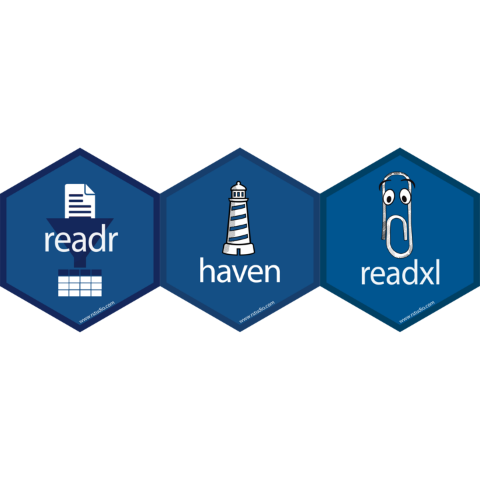
\includegraphics[width=0.5\textwidth,height=\textheight]{fig/import-logo.png}
\caption{\label{fig:import-logo} The logo of the packages readr, haven, and readxl}
\end{figure}

RStudio provides convenient data import tools that can be accessed by clicking \emph{File \textgreater{} Import Dataset}. In addition, tidyverse offers packages for importing data in various formats. This \href{https://posit.co/wp-content/uploads/2022/10/data-import.pdf}{cheatsheet}, for example, is about the packages \texttt{readr}, \texttt{readxl} and \texttt{googlesheets4}. The first allows you to read data in various file formats, including fixed-width files like .csv and .tsv. The package \texttt{readxl} can read in Excel files, i.e., .xls and .xlsx file formats and \texttt{googlesheets4} allows to read and write data from Google Sheets directly from R.

For more information, I recommend once again the second version book \emph{R for Data Science} by \href{https://r4ds.hadley.nz/}{\citet{Wickham2023R}}. In particular, check out the \href{https://r4ds.hadley.nz/data-tidy.html}{``Data tidying''} section for importing CSV and TSV files, the \href{https://r4ds.hadley.nz/spreadsheets.html}{``Spreadsheets''} section for Excel files, the \href{https://r4ds.hadley.nz/databases.html}{``Databases''} section for retrieving data with SQL, the \href{https://r4ds.hadley.nz/arrow.html}{``Arrow''} section for working with large datasets, and the \href{https://r4ds.hadley.nz/webscraping.html}{``Web scraping''} section for extracting data from web pages.

For an overview on packages for reading data that are provided by the tidyverse universe, see \href{https://www.tidyverse.org/packages/\#import}{here}.

\hypertarget{sec:tidy}{%
\section{Data}\label{sec:tidy}}

\hypertarget{data-frames-and-tibbles}{%
\subsection{Data frames and tibbles}\label{data-frames-and-tibbles}}

\begin{figure}
\centering

\includegraphics[width=0.3\textwidth,height=\textheight]{fig/tidyr-tibble-logo.png}
\caption{\label{fig:tidyr-tibble-logo} The logos of the tidyr and tibble packages}
\end{figure}

Both \emph{data frames} and \emph{tibbles} are two of the most commonly used data structures in R for handling tabular data. A tibble actually is a data frame and you can use all functions that work with a data frame also with a tibble. However, a tibble has some additional features in printing and subsetting. Please note, data frames are provided by base R while tibbles are provided by the \texttt{tidyverse} package. This means that if you want to use tibbles you must load \texttt{tidyverse}. It turned out that it is helpful that a tibble has the folllowing features to simplify working with data:
- Each vector is labeled by the variable name.
- Variable names don't have spaces and are not put in quotes.
- All variables have the same length.
- Each variable is of a single type (numeric, character, logical, or a categorical).

\hypertarget{tidy-data}{%
\subsection{Tidy data}\label{tidy-data}}

A popular quote from Hadley Wickham is that \emph{``tidy datasets are all alike, but every messy dataset is messy in its own way''} \citep[p.~2]{Hadley2014Tidy}. It paraphrases the fact that it is a good idea to set rules how a dataset should structure its information to make it easier to work with the data. The tidyverse requires the data to be structured like is illustrated in Figure \ref{fig:tidy-1}. The rules are:

\begin{enumerate}
\def\labelenumi{\arabic{enumi}.}
\tightlist
\item
  Each variable is a column and vice versa.
\item
  Each observation is a row and vice verse.
\item
  Each value is a cell.
\end{enumerate}

\begin{figure}
\centering
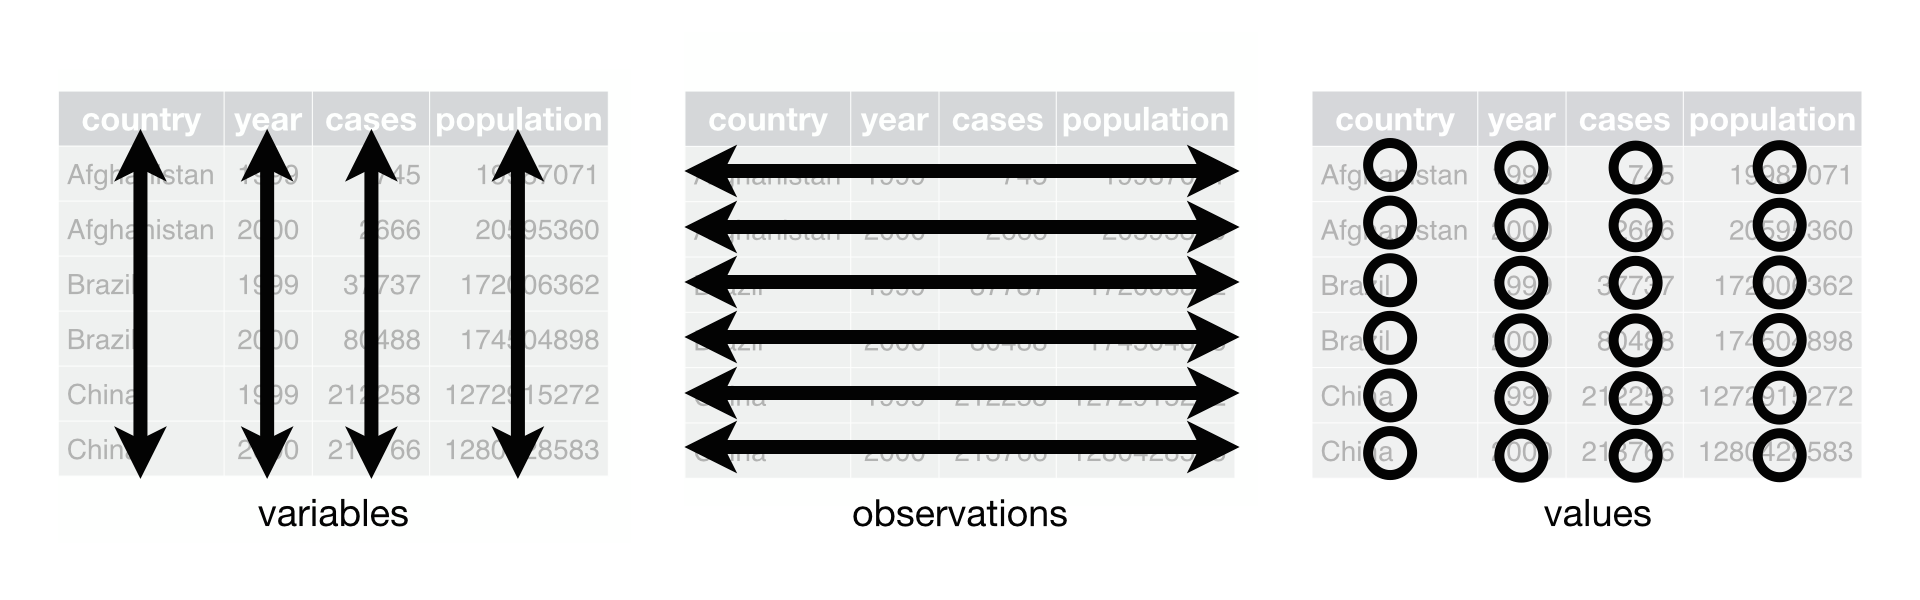
\includegraphics[width=1\textwidth,height=\textheight]{fig/tidy-1.png}
\caption[\label{fig:tidy-1} Features of a tidy dataset: variables are columns, observations are rows, and values are cells]{\label{fig:tidy-1} Features of a tidy dataset: variables are columns, observations are rows, and values are cells\footnotemark{}}
\end{figure}
\footnotetext{The figure stems from \citet{Wickham2023R}}

Whenever data follow that consistent structure, we speak of \emph{tidy data}. The underlying uniformity of tidy data facilitates learning and using data manipulation tools.

One difference between data frames and tibbles is that dataframes store the row names. For example, take the \texttt{mtcars} dataset which consists of 32 different cars and the names of the cars are not stored as rownames:

\begin{Shaded}
\begin{Highlighting}[]
\FunctionTok{class}\NormalTok{(mtcars) }\CommentTok{\# mtcars is a data frame}
\end{Highlighting}
\end{Shaded}

\begin{verbatim}
## [1] "data.frame"
\end{verbatim}

\begin{Shaded}
\begin{Highlighting}[]
\FunctionTok{rownames}\NormalTok{(mtcars) }
\end{Highlighting}
\end{Shaded}

\begin{verbatim}
##  [1] "Mazda RX4"           "Mazda RX4 Wag"       "Datsun 710"          "Hornet 4 Drive"      "Hornet Sportabout"  
##  [6] "Valiant"             "Duster 360"          "Merc 240D"           "Merc 230"            "Merc 280"           
## [11] "Merc 280C"           "Merc 450SE"          "Merc 450SL"          "Merc 450SLC"         "Cadillac Fleetwood" 
## [16] "Lincoln Continental" "Chrysler Imperial"   "Fiat 128"            "Honda Civic"         "Toyota Corolla"     
## [21] "Toyota Corona"       "Dodge Challenger"    "AMC Javelin"         "Camaro Z28"          "Pontiac Firebird"   
## [26] "Fiat X1-9"           "Porsche 914-2"       "Lotus Europa"        "Ford Pantera L"      "Ferrari Dino"       
## [31] "Maserati Bora"       "Volvo 142E"
\end{verbatim}

To store \texttt{mtcars} as a tibble, we can use the \texttt{as\_tibble} function:

\begin{Shaded}
\begin{Highlighting}[]
\NormalTok{tbl\_mtcars }\OtherTok{\textless{}{-}} \FunctionTok{as\_tibble}\NormalTok{(mtcars)}
\FunctionTok{class}\NormalTok{(tbl\_mtcars) }\CommentTok{\# check if it is a tibble now}
\end{Highlighting}
\end{Shaded}

\begin{verbatim}
## [1] "tbl_df"     "tbl"        "data.frame"
\end{verbatim}

\begin{Shaded}
\begin{Highlighting}[]
\FunctionTok{is\_tibble}\NormalTok{(tbl\_mtcars) }\CommentTok{\# alternative check}
\end{Highlighting}
\end{Shaded}

\begin{verbatim}
## [1] TRUE
\end{verbatim}

\begin{Shaded}
\begin{Highlighting}[]
\FunctionTok{head}\NormalTok{(tbl\_mtcars, }\DecValTok{3}\NormalTok{)}
\end{Highlighting}
\end{Shaded}

\begin{verbatim}
## # A tibble: 3 x 11
##     mpg   cyl  disp    hp  drat    wt  qsec    vs    am  gear  carb
##   <dbl> <dbl> <dbl> <dbl> <dbl> <dbl> <dbl> <dbl> <dbl> <dbl> <dbl>
## 1  21       6   160   110  3.9   2.62  16.5     0     1     4     4
## 2  21       6   160   110  3.9   2.88  17.0     0     1     4     4
## 3  22.8     4   108    93  3.85  2.32  18.6     1     1     4     1
\end{verbatim}

When we look at the data, we've lost the names of the cars. To store the these, you need to first add a column to the dataframe containing the rownames and then you can generate the tibble:

\begin{Shaded}
\begin{Highlighting}[]
\NormalTok{tbl\_mtcars }\OtherTok{\textless{}{-}}\NormalTok{ mtcars }\SpecialCharTok{|\textgreater{}} 
  \FunctionTok{rownames\_to\_column}\NormalTok{(}\AttributeTok{var =} \StringTok{"car"}\NormalTok{) }\SpecialCharTok{|\textgreater{}}
  \FunctionTok{as\_tibble}\NormalTok{() }
\FunctionTok{class}\NormalTok{(tbl\_mtcars)}
\end{Highlighting}
\end{Shaded}

\begin{verbatim}
## [1] "tbl_df"     "tbl"        "data.frame"
\end{verbatim}

\begin{Shaded}
\begin{Highlighting}[]
\FunctionTok{head}\NormalTok{(tbl\_mtcars, }\DecValTok{3}\NormalTok{)}
\end{Highlighting}
\end{Shaded}

\begin{verbatim}
## # A tibble: 3 x 12
##   car             mpg   cyl  disp    hp  drat    wt  qsec    vs    am  gear  carb
##   <chr>         <dbl> <dbl> <dbl> <dbl> <dbl> <dbl> <dbl> <dbl> <dbl> <dbl> <dbl>
## 1 Mazda RX4      21       6   160   110  3.9   2.62  16.5     0     1     4     4
## 2 Mazda RX4 Wag  21       6   160   110  3.9   2.88  17.0     0     1     4     4
## 3 Datsun 710     22.8     4   108    93  3.85  2.32  18.6     1     1     4     1
\end{verbatim}

\hypertarget{data-types}{%
\subsection{Data types}\label{data-types}}

In R, different data classes, or types of data exist:

\begin{itemize}
\tightlist
\item
  \emph{numeric}: can be any real number
\item
  \emph{character}: strings and characters
\item
  \emph{integer}: any whole numbers
\item
  \emph{factor}: any categorical or qualitative variable with finite number of distinct outcomes
\item
  \emph{logical}: contain either \texttt{TRUE} or \texttt{FALSE}
\item
  \emph{Date}: special format that describes time
\end{itemize}

The following example should exemplify these types of data:

\begin{Shaded}
\begin{Highlighting}[]
\NormalTok{integer\_var }\OtherTok{\textless{}{-}} \FunctionTok{c}\NormalTok{(}\DecValTok{1}\NormalTok{, }\DecValTok{2}\NormalTok{, }\DecValTok{3}\NormalTok{, }\DecValTok{4}\NormalTok{, }\DecValTok{5}\NormalTok{)}
\NormalTok{numeric\_var }\OtherTok{\textless{}{-}} \FunctionTok{c}\NormalTok{(}\FloatTok{1.1}\NormalTok{, }\FloatTok{2.2}\NormalTok{, }\ConstantTok{NA}\NormalTok{, }\FloatTok{4.4}\NormalTok{, }\FloatTok{5.5}\NormalTok{)}
\NormalTok{character\_var }\OtherTok{\textless{}{-}} \FunctionTok{c}\NormalTok{(}\StringTok{"apple"}\NormalTok{, }\StringTok{"banana"}\NormalTok{, }\StringTok{"orange"}\NormalTok{, }\StringTok{"cherry"}\NormalTok{, }\StringTok{"grape"}\NormalTok{)}
\NormalTok{factor\_var }\OtherTok{\textless{}{-}} \FunctionTok{factor}\NormalTok{(}\FunctionTok{c}\NormalTok{(}\StringTok{"red"}\NormalTok{, }\StringTok{"yellow"}\NormalTok{, }\StringTok{"red"}\NormalTok{, }\StringTok{"blue"}\NormalTok{, }\StringTok{"green"}\NormalTok{))}
\NormalTok{logical\_var }\OtherTok{\textless{}{-}} \FunctionTok{c}\NormalTok{(}\ConstantTok{TRUE}\NormalTok{, }\ConstantTok{TRUE}\NormalTok{, }\ConstantTok{TRUE}\NormalTok{, }\ConstantTok{FALSE}\NormalTok{, }\ConstantTok{TRUE}\NormalTok{)}
\NormalTok{date\_var }\OtherTok{\textless{}{-}} \FunctionTok{as.Date}\NormalTok{(}\FunctionTok{c}\NormalTok{(}\StringTok{"2022{-}01{-}01"}\NormalTok{, }\StringTok{"2022{-}02{-}01"}\NormalTok{, }\StringTok{"2022{-}03{-}01"}\NormalTok{, }\StringTok{"2022{-}04{-}01"}\NormalTok{, }\StringTok{"2022{-}05{-}01"}\NormalTok{))}

\NormalTok{date\_var[}\DecValTok{2}\NormalTok{] }\SpecialCharTok{{-}}\NormalTok{ date\_var[}\DecValTok{5}\NormalTok{] }\CommentTok{\# number of days in between these two dates}
\end{Highlighting}
\end{Shaded}

\begin{verbatim}
## Time difference of -89 days
\end{verbatim}

There are some special data values used in R that needs further explanation:

\begin{itemize}
\tightlist
\item
  \texttt{NA} stands for \emph{not available} or \emph{missing} and is used to represent missing or undefined values.
\item
  \texttt{Inf} stands for \emph{infinity} and is used to represent mathematical infinity, such as the result of dividing a non-zero number by zero. Can be positive or negative.\\
\item
  \texttt{NULL} represents an empty or non-existent object. It is often used as a placeholder when a value or object is not yet available or when an object is intentionally removed.
\item
  \texttt{NaN} stands for \emph{not a number} and is used to represent an undefined or unrepresentable value, such as the result of taking the square root of a negative number. It can also occur as a result of certain arithmetic operations that are undefined. In contrast to \texttt{NA} it can only exist in numerical data.
\end{itemize}

\hypertarget{tools-to-manipulate-data}{%
\section{Tools to manipulate data}\label{tools-to-manipulate-data}}

\hypertarget{the-in-operator}{%
\subsection{\texorpdfstring{The \texttt{\%in\%} operator}{The \%in\% operator}}\label{the-in-operator}}

\texttt{\%in\%} is used to subset a vector by comparison. Here's an example:

\begin{Shaded}
\begin{Highlighting}[]
\NormalTok{x }\OtherTok{\textless{}{-}} \FunctionTok{c}\NormalTok{(}\DecValTok{1}\NormalTok{, }\DecValTok{3}\NormalTok{, }\DecValTok{5}\NormalTok{, }\DecValTok{7}\NormalTok{)}
\NormalTok{y }\OtherTok{\textless{}{-}} \FunctionTok{c}\NormalTok{(}\DecValTok{2}\NormalTok{, }\DecValTok{4}\NormalTok{, }\DecValTok{6}\NormalTok{, }\DecValTok{8}\NormalTok{)}
\NormalTok{z }\OtherTok{\textless{}{-}} \FunctionTok{c}\NormalTok{(}\DecValTok{1}\NormalTok{, }\DecValTok{2}\NormalTok{, }\DecValTok{3}\NormalTok{)}

\NormalTok{x }\SpecialCharTok{\%in\%}\NormalTok{ y  }
\end{Highlighting}
\end{Shaded}

\begin{verbatim}
## [1] FALSE FALSE FALSE FALSE
\end{verbatim}

\begin{Shaded}
\begin{Highlighting}[]
\NormalTok{x }\SpecialCharTok{\%in\%}\NormalTok{ z  }
\end{Highlighting}
\end{Shaded}

\begin{verbatim}
## [1]  TRUE  TRUE FALSE FALSE
\end{verbatim}

\begin{Shaded}
\begin{Highlighting}[]
\NormalTok{z }\SpecialCharTok{\%in\%}\NormalTok{ x}
\end{Highlighting}
\end{Shaded}

\begin{verbatim}
## [1]  TRUE FALSE  TRUE
\end{verbatim}

The \%in\% operator can be used in combination with other functions like \texttt{subset()} and \texttt{filter()}.

\hypertarget{extract-operators}{%
\subsection{Extract operators}\label{extract-operators}}

The \emph{extract operators} are used to retrieve data from objects in R. The operator may take four forms, including \texttt{{[}{]}}, \texttt{{[}{[}{]}{]}}, and \texttt{\$}.

\texttt{{[}{]}} allows to extract content from vector, lists, or data frames. For example,

\begin{Shaded}
\begin{Highlighting}[]
\NormalTok{a }\OtherTok{\textless{}{-}}\NormalTok{ mtcars[}\DecValTok{3}\NormalTok{, ]}
\NormalTok{b }\OtherTok{\textless{}{-}}\NormalTok{ mtcars[}\StringTok{"Datsun 710"}\NormalTok{, ]}
\FunctionTok{identical}\NormalTok{(a, b)}
\end{Highlighting}
\end{Shaded}

\begin{verbatim}
## [1] TRUE
\end{verbatim}

\begin{Shaded}
\begin{Highlighting}[]
\NormalTok{a}
\end{Highlighting}
\end{Shaded}

\begin{verbatim}
##             mpg cyl disp hp drat   wt  qsec vs am gear carb
## Datsun 710 22.8   4  108 93 3.85 2.32 18.61  1  1    4    1
\end{verbatim}

extracts the third observation of the mtcars dataset, and

\begin{Shaded}
\begin{Highlighting}[]
\NormalTok{c }\OtherTok{\textless{}{-}}\NormalTok{ mtcars[,}\StringTok{"cyl"}\NormalTok{]}
\NormalTok{d }\OtherTok{\textless{}{-}}\NormalTok{ mtcars[, }\DecValTok{2}\NormalTok{]}
\FunctionTok{identical}\NormalTok{(x, y)}
\end{Highlighting}
\end{Shaded}

\begin{verbatim}
## [1] FALSE
\end{verbatim}

\begin{Shaded}
\begin{Highlighting}[]
\NormalTok{c}
\end{Highlighting}
\end{Shaded}

\begin{verbatim}
##  [1] 6 6 4 6 8 6 8 4 4 6 6 8 8 8 8 8 8 4 4 4 4 8 8 8 8 4 4 4 8 6 8 4
\end{verbatim}

extracts the variable/vector \texttt{cyl}.

The operators, \texttt{{[}{[}{]}{]}} and \texttt{\$} extract a single item from an object. It is used to refer to an element in a list or a column in a data frame. For example,

\begin{Shaded}
\begin{Highlighting}[]
\NormalTok{e }\OtherTok{\textless{}{-}}\NormalTok{ mtcars}\SpecialCharTok{$}\NormalTok{cyl}
\NormalTok{f }\OtherTok{\textless{}{-}}\NormalTok{ mtcars[[}\StringTok{"cyl"}\NormalTok{]]}
\FunctionTok{identical}\NormalTok{(e, f)}
\end{Highlighting}
\end{Shaded}

\begin{verbatim}
## [1] TRUE
\end{verbatim}

\begin{Shaded}
\begin{Highlighting}[]
\NormalTok{e}
\end{Highlighting}
\end{Shaded}

\begin{verbatim}
##  [1] 6 6 4 6 8 6 8 4 4 6 6 8 8 8 8 8 8 4 4 4 4 8 8 8 8 4 4 4 8 6 8 4
\end{verbatim}

will return the values of the variable \texttt{cyl} from the data frame \texttt{mtcars}.
Thus, x\$y is actually just a short form for x{[}{[}``y''{]}{]}.

\hypertarget{logical-operators}{%
\subsection{Logical operators}\label{logical-operators}}

The extract operators can be combined with the \emph{logical operators} (more precisely, I should call these \emph{binary relational operators}) that are shown in table Table 1.

\begin{longtable}[]{@{}
  >{\raggedright\arraybackslash}p{(\columnwidth - 6\tabcolsep) * \real{0.3553}}
  >{\raggedright\arraybackslash}p{(\columnwidth - 6\tabcolsep) * \real{0.1447}}
  >{\raggedright\arraybackslash}p{(\columnwidth - 6\tabcolsep) * \real{0.3553}}
  >{\raggedright\arraybackslash}p{(\columnwidth - 6\tabcolsep) * \real{0.1447}}@{}}
\caption{Table 1: Logical operators}\tabularnewline
\toprule\noalign{}
\begin{minipage}[b]{\linewidth}\raggedright
operation
\end{minipage} & \begin{minipage}[b]{\linewidth}\raggedright
operator
\end{minipage} & \begin{minipage}[b]{\linewidth}\raggedright
example input
\end{minipage} & \begin{minipage}[b]{\linewidth}\raggedright
answer
\end{minipage} \\
\midrule\noalign{}
\endfirsthead
\toprule\noalign{}
\begin{minipage}[b]{\linewidth}\raggedright
operation
\end{minipage} & \begin{minipage}[b]{\linewidth}\raggedright
operator
\end{minipage} & \begin{minipage}[b]{\linewidth}\raggedright
example input
\end{minipage} & \begin{minipage}[b]{\linewidth}\raggedright
answer
\end{minipage} \\
\midrule\noalign{}
\endhead
\bottomrule\noalign{}
\endlastfoot
less than & \texttt{\textless{}} & \texttt{2\ \textless{}\ 3} & \texttt{TRUE} \\
less than or equal to & \texttt{\textless{}=} & \texttt{2\ \textless{}=\ 2} & \texttt{TRUE} \\
greater than & \texttt{\textgreater{}} & \texttt{2\ \textgreater{}\ 3} & \texttt{FALSE} \\
greater than or equal to & \texttt{\textgreater{}=} & \texttt{2\ \textgreater{}=\ 2} & \texttt{TRUE} \\
equal to & \texttt{==} & \texttt{2\ ==\ 3} & \texttt{FALSE} \\
not equal to & \texttt{!=} & \texttt{2\ !=\ 3} & \texttt{TRUE} \\
& & & \\
not & \texttt{!} & \texttt{!(1==1)} & \texttt{FALSE} \\
or & \(\vert\) & \texttt{(1==1)} \(\vert\) \texttt{(2==3)} & \texttt{TRUE} \\
and & \texttt{\&} & \texttt{(1==1)\ \&\ (2==3)} & \texttt{FALSE} \\
\end{longtable}

Here are some examples:
Select rows where the number of cylinders is greater than or equal to 6:

\begin{Shaded}
\begin{Highlighting}[]
\NormalTok{mtcars[mtcars}\SpecialCharTok{$}\NormalTok{cyl }\SpecialCharTok{\textgreater{}=} \DecValTok{6}\NormalTok{, ]}
\end{Highlighting}
\end{Shaded}

\begin{verbatim}
##                      mpg cyl  disp  hp drat    wt  qsec vs am gear carb
## Mazda RX4           21.0   6 160.0 110 3.90 2.620 16.46  0  1    4    4
## Mazda RX4 Wag       21.0   6 160.0 110 3.90 2.875 17.02  0  1    4    4
## Hornet 4 Drive      21.4   6 258.0 110 3.08 3.215 19.44  1  0    3    1
## Hornet Sportabout   18.7   8 360.0 175 3.15 3.440 17.02  0  0    3    2
## Valiant             18.1   6 225.0 105 2.76 3.460 20.22  1  0    3    1
## Duster 360          14.3   8 360.0 245 3.21 3.570 15.84  0  0    3    4
## Merc 280            19.2   6 167.6 123 3.92 3.440 18.30  1  0    4    4
## Merc 280C           17.8   6 167.6 123 3.92 3.440 18.90  1  0    4    4
## Merc 450SE          16.4   8 275.8 180 3.07 4.070 17.40  0  0    3    3
## Merc 450SL          17.3   8 275.8 180 3.07 3.730 17.60  0  0    3    3
## Merc 450SLC         15.2   8 275.8 180 3.07 3.780 18.00  0  0    3    3
## Cadillac Fleetwood  10.4   8 472.0 205 2.93 5.250 17.98  0  0    3    4
## Lincoln Continental 10.4   8 460.0 215 3.00 5.424 17.82  0  0    3    4
## Chrysler Imperial   14.7   8 440.0 230 3.23 5.345 17.42  0  0    3    4
## Dodge Challenger    15.5   8 318.0 150 2.76 3.520 16.87  0  0    3    2
## AMC Javelin         15.2   8 304.0 150 3.15 3.435 17.30  0  0    3    2
## Camaro Z28          13.3   8 350.0 245 3.73 3.840 15.41  0  0    3    4
## Pontiac Firebird    19.2   8 400.0 175 3.08 3.845 17.05  0  0    3    2
## Ford Pantera L      15.8   8 351.0 264 4.22 3.170 14.50  0  1    5    4
## Ferrari Dino        19.7   6 145.0 175 3.62 2.770 15.50  0  1    5    6
## Maserati Bora       15.0   8 301.0 335 3.54 3.570 14.60  0  1    5    8
\end{verbatim}

Select rows where the number of cylinders is either 4 or 6:

\begin{Shaded}
\begin{Highlighting}[]
\NormalTok{mtcars[mtcars}\SpecialCharTok{$}\NormalTok{cyl }\SpecialCharTok{==} \DecValTok{4} \SpecialCharTok{|}\NormalTok{ mtcars}\SpecialCharTok{$}\NormalTok{cyl }\SpecialCharTok{==} \DecValTok{6}\NormalTok{ , ]}
\end{Highlighting}
\end{Shaded}

\begin{verbatim}
##                 mpg cyl  disp  hp drat    wt  qsec vs am gear carb
## Mazda RX4      21.0   6 160.0 110 3.90 2.620 16.46  0  1    4    4
## Mazda RX4 Wag  21.0   6 160.0 110 3.90 2.875 17.02  0  1    4    4
## Datsun 710     22.8   4 108.0  93 3.85 2.320 18.61  1  1    4    1
## Hornet 4 Drive 21.4   6 258.0 110 3.08 3.215 19.44  1  0    3    1
## Valiant        18.1   6 225.0 105 2.76 3.460 20.22  1  0    3    1
## Merc 240D      24.4   4 146.7  62 3.69 3.190 20.00  1  0    4    2
## Merc 230       22.8   4 140.8  95 3.92 3.150 22.90  1  0    4    2
## Merc 280       19.2   6 167.6 123 3.92 3.440 18.30  1  0    4    4
## Merc 280C      17.8   6 167.6 123 3.92 3.440 18.90  1  0    4    4
## Fiat 128       32.4   4  78.7  66 4.08 2.200 19.47  1  1    4    1
## Honda Civic    30.4   4  75.7  52 4.93 1.615 18.52  1  1    4    2
## Toyota Corolla 33.9   4  71.1  65 4.22 1.835 19.90  1  1    4    1
## Toyota Corona  21.5   4 120.1  97 3.70 2.465 20.01  1  0    3    1
## Fiat X1-9      27.3   4  79.0  66 4.08 1.935 18.90  1  1    4    1
## Porsche 914-2  26.0   4 120.3  91 4.43 2.140 16.70  0  1    5    2
## Lotus Europa   30.4   4  95.1 113 3.77 1.513 16.90  1  1    5    2
## Ferrari Dino   19.7   6 145.0 175 3.62 2.770 15.50  0  1    5    6
## Volvo 142E     21.4   4 121.0 109 4.11 2.780 18.60  1  1    4    2
\end{verbatim}

Select rows where the number of cylinders is 4 and the mpg is greater than 22:

\begin{Shaded}
\begin{Highlighting}[]
\NormalTok{mtcars[mtcars}\SpecialCharTok{$}\NormalTok{cyl }\SpecialCharTok{==} \DecValTok{4} \SpecialCharTok{\&}\NormalTok{ mtcars}\SpecialCharTok{$}\NormalTok{mpg }\SpecialCharTok{\textgreater{}} \DecValTok{22}\NormalTok{, ]}
\end{Highlighting}
\end{Shaded}

\begin{verbatim}
##                 mpg cyl  disp  hp drat    wt  qsec vs am gear carb
## Datsun 710     22.8   4 108.0  93 3.85 2.320 18.61  1  1    4    1
## Merc 240D      24.4   4 146.7  62 3.69 3.190 20.00  1  0    4    2
## Merc 230       22.8   4 140.8  95 3.92 3.150 22.90  1  0    4    2
## Fiat 128       32.4   4  78.7  66 4.08 2.200 19.47  1  1    4    1
## Honda Civic    30.4   4  75.7  52 4.93 1.615 18.52  1  1    4    2
## Toyota Corolla 33.9   4  71.1  65 4.22 1.835 19.90  1  1    4    1
## Fiat X1-9      27.3   4  79.0  66 4.08 1.935 18.90  1  1    4    1
## Porsche 914-2  26.0   4 120.3  91 4.43 2.140 16.70  0  1    5    2
## Lotus Europa   30.4   4  95.1 113 3.77 1.513 16.90  1  1    5    2
\end{verbatim}

Select rows where the weight is less than 3.5 or the number of gears is greater than 4:

\begin{Shaded}
\begin{Highlighting}[]
\NormalTok{mtcars[mtcars}\SpecialCharTok{$}\NormalTok{wt }\SpecialCharTok{\textless{}} \FloatTok{3.5} \SpecialCharTok{|}\NormalTok{ mtcars}\SpecialCharTok{$}\NormalTok{gear }\SpecialCharTok{\textgreater{}} \DecValTok{4}\NormalTok{, ]}
\end{Highlighting}
\end{Shaded}

\begin{verbatim}
##                    mpg cyl  disp  hp drat    wt  qsec vs am gear carb
## Mazda RX4         21.0   6 160.0 110 3.90 2.620 16.46  0  1    4    4
## Mazda RX4 Wag     21.0   6 160.0 110 3.90 2.875 17.02  0  1    4    4
## Datsun 710        22.8   4 108.0  93 3.85 2.320 18.61  1  1    4    1
## Hornet 4 Drive    21.4   6 258.0 110 3.08 3.215 19.44  1  0    3    1
## Hornet Sportabout 18.7   8 360.0 175 3.15 3.440 17.02  0  0    3    2
## Valiant           18.1   6 225.0 105 2.76 3.460 20.22  1  0    3    1
## Merc 240D         24.4   4 146.7  62 3.69 3.190 20.00  1  0    4    2
## Merc 230          22.8   4 140.8  95 3.92 3.150 22.90  1  0    4    2
## Merc 280          19.2   6 167.6 123 3.92 3.440 18.30  1  0    4    4
## Merc 280C         17.8   6 167.6 123 3.92 3.440 18.90  1  0    4    4
## Fiat 128          32.4   4  78.7  66 4.08 2.200 19.47  1  1    4    1
## Honda Civic       30.4   4  75.7  52 4.93 1.615 18.52  1  1    4    2
## Toyota Corolla    33.9   4  71.1  65 4.22 1.835 19.90  1  1    4    1
## Toyota Corona     21.5   4 120.1  97 3.70 2.465 20.01  1  0    3    1
## AMC Javelin       15.2   8 304.0 150 3.15 3.435 17.30  0  0    3    2
## Fiat X1-9         27.3   4  79.0  66 4.08 1.935 18.90  1  1    4    1
## Porsche 914-2     26.0   4 120.3  91 4.43 2.140 16.70  0  1    5    2
## Lotus Europa      30.4   4  95.1 113 3.77 1.513 16.90  1  1    5    2
## Ford Pantera L    15.8   8 351.0 264 4.22 3.170 14.50  0  1    5    4
## Ferrari Dino      19.7   6 145.0 175 3.62 2.770 15.50  0  1    5    6
## Maserati Bora     15.0   8 301.0 335 3.54 3.570 14.60  0  1    5    8
## Volvo 142E        21.4   4 121.0 109 4.11 2.780 18.60  1  1    4    2
\end{verbatim}

Select rows where either mpg is greater than 25 or carb is less than 2, and the number of cylinders is either 4 or 8.

\begin{Shaded}
\begin{Highlighting}[]
\NormalTok{mtcars[(mtcars}\SpecialCharTok{$}\NormalTok{mpg }\SpecialCharTok{\textgreater{}} \DecValTok{25} \SpecialCharTok{|}\NormalTok{ mtcars}\SpecialCharTok{$}\NormalTok{carb }\SpecialCharTok{\textless{}} \DecValTok{2}\NormalTok{) }\SpecialCharTok{\&}\NormalTok{ mtcars}\SpecialCharTok{$}\NormalTok{cyl }\SpecialCharTok{\%in\%} \FunctionTok{c}\NormalTok{(}\DecValTok{4}\NormalTok{,}\DecValTok{8}\NormalTok{), ]}
\end{Highlighting}
\end{Shaded}

\begin{verbatim}
##                 mpg cyl  disp  hp drat    wt  qsec vs am gear carb
## Datsun 710     22.8   4 108.0  93 3.85 2.320 18.61  1  1    4    1
## Fiat 128       32.4   4  78.7  66 4.08 2.200 19.47  1  1    4    1
## Honda Civic    30.4   4  75.7  52 4.93 1.615 18.52  1  1    4    2
## Toyota Corolla 33.9   4  71.1  65 4.22 1.835 19.90  1  1    4    1
## Toyota Corona  21.5   4 120.1  97 3.70 2.465 20.01  1  0    3    1
## Fiat X1-9      27.3   4  79.0  66 4.08 1.935 18.90  1  1    4    1
## Porsche 914-2  26.0   4 120.3  91 4.43 2.140 16.70  0  1    5    2
## Lotus Europa   30.4   4  95.1 113 3.77 1.513 16.90  1  1    5    2
\end{verbatim}

\hypertarget{if-statements}{%
\subsection{If statements}\label{if-statements}}

In many cases, it's necessary to execute certain code only when a particular condition is met. To achieve this, there are several conditional statements that can be used in code. These include:

\begin{itemize}
\tightlist
\item
  The \texttt{if} statement: This is used to execute a block of code if a specified condition is true.
\item
  The \texttt{else} statement: This is used to execute a block of code if the same condition is false.
\item
  The \texttt{else} if statement: This is used to specify a new condition to test if the first condition is false.
\item
  The \texttt{ifelse()} function: This is used to check a condition for every element of a vector.
\end{itemize}

The following examples should exemplify how these statements work:

\begin{Shaded}
\begin{Highlighting}[]
\CommentTok{\# Example of if statement}
\ControlFlowTok{if}\NormalTok{ (}\FunctionTok{mean}\NormalTok{(mtcars}\SpecialCharTok{$}\NormalTok{mpg) }\SpecialCharTok{\textgreater{}} \DecValTok{20}\NormalTok{) \{}
  \FunctionTok{print}\NormalTok{(}\StringTok{"The average miles per gallon is greater than 20."}\NormalTok{)}
\NormalTok{\}}
\end{Highlighting}
\end{Shaded}

\begin{verbatim}
## [1] "The average miles per gallon is greater than 20."
\end{verbatim}

\begin{Shaded}
\begin{Highlighting}[]
\CommentTok{\# Example of if{-}else statement}
\ControlFlowTok{if}\NormalTok{ (}\FunctionTok{mean}\NormalTok{(mtcars}\SpecialCharTok{$}\NormalTok{mpg) }\SpecialCharTok{\textgreater{}} \DecValTok{20}\NormalTok{) \{}
  \FunctionTok{print}\NormalTok{(}\StringTok{"The average miles per gallon is greater than 20."}\NormalTok{)}
\NormalTok{\} }\ControlFlowTok{else}\NormalTok{ \{}
  \FunctionTok{print}\NormalTok{(}\StringTok{"The average miles per gallon is less than or equal to 20."}\NormalTok{)}
\NormalTok{\}}
\end{Highlighting}
\end{Shaded}

\begin{verbatim}
## [1] "The average miles per gallon is greater than 20."
\end{verbatim}

\begin{Shaded}
\begin{Highlighting}[]
\CommentTok{\# Example of if{-}else if statement}
\ControlFlowTok{if}\NormalTok{ (}\FunctionTok{mean}\NormalTok{(mtcars}\SpecialCharTok{$}\NormalTok{mpg) }\SpecialCharTok{\textgreater{}} \DecValTok{25}\NormalTok{) \{}
  \FunctionTok{print}\NormalTok{(}\StringTok{"The average miles per gallon is greater than 25."}\NormalTok{)}
\NormalTok{\} }\ControlFlowTok{else} \ControlFlowTok{if}\NormalTok{ (}\FunctionTok{mean}\NormalTok{(mtcars}\SpecialCharTok{$}\NormalTok{mpg) }\SpecialCharTok{\textgreater{}} \DecValTok{20}\NormalTok{) \{}
  \FunctionTok{print}\NormalTok{(}\StringTok{"The average miles per gallon is between 20 and 25."}\NormalTok{)}
\NormalTok{\} }\ControlFlowTok{else}\NormalTok{ \{}
  \FunctionTok{print}\NormalTok{(}\StringTok{"The average miles per gallon is less than or equal to 20."}\NormalTok{)}
\NormalTok{\}}
\end{Highlighting}
\end{Shaded}

\begin{verbatim}
## [1] "The average miles per gallon is between 20 and 25."
\end{verbatim}

\begin{Shaded}
\begin{Highlighting}[]
\CommentTok{\# Example of if\_else function}
\NormalTok{mtcars\_2 }\OtherTok{\textless{}{-}}\NormalTok{ mtcars}
\NormalTok{mtcars\_2}\SpecialCharTok{$}\NormalTok{mpg\_category }\OtherTok{\textless{}{-}} \FunctionTok{ifelse}\NormalTok{(mtcars\_2}\SpecialCharTok{$}\NormalTok{mpg }\SpecialCharTok{\textgreater{}} \DecValTok{20}\NormalTok{, }\StringTok{"High"}\NormalTok{, }\StringTok{"Low"}\NormalTok{)}
\end{Highlighting}
\end{Shaded}

When you have a fixed number of cases and don't want to use a long chain of if-else statements, you can use \texttt{case\_when()};

\begin{Shaded}
\begin{Highlighting}[]
\NormalTok{mtcars\_cyl }\OtherTok{\textless{}{-}}\NormalTok{ mtcars }\SpecialCharTok{\%\textgreater{}\%}
  \FunctionTok{mutate}\NormalTok{(}\AttributeTok{cyl\_category =} \FunctionTok{case\_when}\NormalTok{(}
\NormalTok{    cyl }\SpecialCharTok{==} \DecValTok{4} \SpecialCharTok{\textasciitilde{}} \StringTok{"four"}\NormalTok{,}
\NormalTok{    cyl }\SpecialCharTok{==} \DecValTok{6} \SpecialCharTok{\textasciitilde{}} \StringTok{"six"}\NormalTok{,}
\NormalTok{    cyl }\SpecialCharTok{==} \DecValTok{8} \SpecialCharTok{\textasciitilde{}} \StringTok{"eight"}
\NormalTok{  ))}
\end{Highlighting}
\end{Shaded}

The \texttt{mutate()} function is used to add the new variable, and \texttt{case\_when()} is used to assign the values ``four'', ``six'', or ``eight'' to the new variable based on the number of cylinders in each car.

It evaluates one of several expressions based on the value of a given control expression. It takes two arguments: the control expression and a list of named expressions, each of which is evaluated if its name matches the value of the control expression. If no match is found, an optional default expression is evaluated. The switch() function is particularly useful

\hypertarget{data-manipulation-with-dplyr}{%
\section{Data manipulation with dplyr}\label{data-manipulation-with-dplyr}}

\begin{figure}
\centering

\includegraphics[width=0.2\textwidth,height=\textheight]{fig/dplyr-logo.png}
\caption{\label{fig:dplyr-logo} The logo of the dplyr package}
\end{figure}

The dplyr package is part of tidyverse and makes data manipulation easy:

\begin{itemize}
\tightlist
\item
  Reorder the rows (\texttt{arrange()}).
\item
  Pick observations by their values (\texttt{filter()}).
\item
  Pick variables by their names (\texttt{select()}).
\item
  Create new variables with functions of existing variables
  (\texttt{mutate()}).
\item
  Collapse many values down to a single summary (\texttt{summarise()}).
\item
  Rename variables (\texttt{rename()}).
\end{itemize}

These functions can all be used in conjunction with \texttt{group\_by()} , which changes the scope of each function from operating on the entire dataset to operating on it group-by-group.

All functions work similarly:

\begin{enumerate}
\def\labelenumi{\arabic{enumi}.}
\tightlist
\item
  The first argument is a data frame.
\item
  The subsequent arguments describe what to do with the data frame.
\item
  The result is a new data frame.
\end{enumerate}

Here are some examples that may help to understand these functions:

\begin{Shaded}
\begin{Highlighting}[]
\FunctionTok{library}\NormalTok{(tidyverse)}

\CommentTok{\# load mtcars dataset}
\FunctionTok{data}\NormalTok{(mtcars)}

\CommentTok{\# arrange rows by mpg in descending order}
\NormalTok{mtcars }\SpecialCharTok{|\textgreater{}} 
  \FunctionTok{arrange}\NormalTok{(}\FunctionTok{desc}\NormalTok{(mpg))}
\end{Highlighting}
\end{Shaded}

\begin{verbatim}
##                      mpg cyl  disp  hp drat    wt  qsec vs am gear carb
## Toyota Corolla      33.9   4  71.1  65 4.22 1.835 19.90  1  1    4    1
## Fiat 128            32.4   4  78.7  66 4.08 2.200 19.47  1  1    4    1
## Honda Civic         30.4   4  75.7  52 4.93 1.615 18.52  1  1    4    2
## Lotus Europa        30.4   4  95.1 113 3.77 1.513 16.90  1  1    5    2
## Fiat X1-9           27.3   4  79.0  66 4.08 1.935 18.90  1  1    4    1
## Porsche 914-2       26.0   4 120.3  91 4.43 2.140 16.70  0  1    5    2
## Merc 240D           24.4   4 146.7  62 3.69 3.190 20.00  1  0    4    2
## Datsun 710          22.8   4 108.0  93 3.85 2.320 18.61  1  1    4    1
## Merc 230            22.8   4 140.8  95 3.92 3.150 22.90  1  0    4    2
## Toyota Corona       21.5   4 120.1  97 3.70 2.465 20.01  1  0    3    1
## Hornet 4 Drive      21.4   6 258.0 110 3.08 3.215 19.44  1  0    3    1
## Volvo 142E          21.4   4 121.0 109 4.11 2.780 18.60  1  1    4    2
## Mazda RX4           21.0   6 160.0 110 3.90 2.620 16.46  0  1    4    4
## Mazda RX4 Wag       21.0   6 160.0 110 3.90 2.875 17.02  0  1    4    4
## Ferrari Dino        19.7   6 145.0 175 3.62 2.770 15.50  0  1    5    6
## Merc 280            19.2   6 167.6 123 3.92 3.440 18.30  1  0    4    4
## Pontiac Firebird    19.2   8 400.0 175 3.08 3.845 17.05  0  0    3    2
## Hornet Sportabout   18.7   8 360.0 175 3.15 3.440 17.02  0  0    3    2
## Valiant             18.1   6 225.0 105 2.76 3.460 20.22  1  0    3    1
## Merc 280C           17.8   6 167.6 123 3.92 3.440 18.90  1  0    4    4
## Merc 450SL          17.3   8 275.8 180 3.07 3.730 17.60  0  0    3    3
## Merc 450SE          16.4   8 275.8 180 3.07 4.070 17.40  0  0    3    3
## Ford Pantera L      15.8   8 351.0 264 4.22 3.170 14.50  0  1    5    4
## Dodge Challenger    15.5   8 318.0 150 2.76 3.520 16.87  0  0    3    2
## Merc 450SLC         15.2   8 275.8 180 3.07 3.780 18.00  0  0    3    3
## AMC Javelin         15.2   8 304.0 150 3.15 3.435 17.30  0  0    3    2
## Maserati Bora       15.0   8 301.0 335 3.54 3.570 14.60  0  1    5    8
## Chrysler Imperial   14.7   8 440.0 230 3.23 5.345 17.42  0  0    3    4
## Duster 360          14.3   8 360.0 245 3.21 3.570 15.84  0  0    3    4
## Camaro Z28          13.3   8 350.0 245 3.73 3.840 15.41  0  0    3    4
## Cadillac Fleetwood  10.4   8 472.0 205 2.93 5.250 17.98  0  0    3    4
## Lincoln Continental 10.4   8 460.0 215 3.00 5.424 17.82  0  0    3    4
\end{verbatim}

\begin{Shaded}
\begin{Highlighting}[]
\CommentTok{\# filter rows where cyl = 4}
\NormalTok{mtcars }\SpecialCharTok{|\textgreater{}} 
  \FunctionTok{filter}\NormalTok{(cyl }\SpecialCharTok{==} \DecValTok{4}\NormalTok{)}
\end{Highlighting}
\end{Shaded}

\begin{verbatim}
##                 mpg cyl  disp  hp drat    wt  qsec vs am gear carb
## Datsun 710     22.8   4 108.0  93 3.85 2.320 18.61  1  1    4    1
## Merc 240D      24.4   4 146.7  62 3.69 3.190 20.00  1  0    4    2
## Merc 230       22.8   4 140.8  95 3.92 3.150 22.90  1  0    4    2
## Fiat 128       32.4   4  78.7  66 4.08 2.200 19.47  1  1    4    1
## Honda Civic    30.4   4  75.7  52 4.93 1.615 18.52  1  1    4    2
## Toyota Corolla 33.9   4  71.1  65 4.22 1.835 19.90  1  1    4    1
## Toyota Corona  21.5   4 120.1  97 3.70 2.465 20.01  1  0    3    1
## Fiat X1-9      27.3   4  79.0  66 4.08 1.935 18.90  1  1    4    1
## Porsche 914-2  26.0   4 120.3  91 4.43 2.140 16.70  0  1    5    2
## Lotus Europa   30.4   4  95.1 113 3.77 1.513 16.90  1  1    5    2
## Volvo 142E     21.4   4 121.0 109 4.11 2.780 18.60  1  1    4    2
\end{verbatim}

\begin{Shaded}
\begin{Highlighting}[]
\CommentTok{\# select columns mpg, cyl, and hp}
\NormalTok{mtcars }\SpecialCharTok{|\textgreater{}} 
  \FunctionTok{select}\NormalTok{(mpg, cyl, hp) }\SpecialCharTok{|\textgreater{}} 
  \FunctionTok{head}\NormalTok{()}
\end{Highlighting}
\end{Shaded}

\begin{verbatim}
##                    mpg cyl  hp
## Mazda RX4         21.0   6 110
## Mazda RX4 Wag     21.0   6 110
## Datsun 710        22.8   4  93
## Hornet 4 Drive    21.4   6 110
## Hornet Sportabout 18.7   8 175
## Valiant           18.1   6 105
\end{verbatim}

\begin{Shaded}
\begin{Highlighting}[]
\CommentTok{\# select columns all variables except wt and hp}
\NormalTok{mtcars }\SpecialCharTok{|\textgreater{}} 
  \FunctionTok{select}\NormalTok{(}\SpecialCharTok{{-}}\NormalTok{wt, }\SpecialCharTok{{-}}\NormalTok{hp) }\SpecialCharTok{|\textgreater{}} 
  \FunctionTok{head}\NormalTok{()}
\end{Highlighting}
\end{Shaded}

\begin{verbatim}
##                    mpg cyl disp drat  qsec vs am gear carb
## Mazda RX4         21.0   6  160 3.90 16.46  0  1    4    4
## Mazda RX4 Wag     21.0   6  160 3.90 17.02  0  1    4    4
## Datsun 710        22.8   4  108 3.85 18.61  1  1    4    1
## Hornet 4 Drive    21.4   6  258 3.08 19.44  1  0    3    1
## Hornet Sportabout 18.7   8  360 3.15 17.02  0  0    3    2
## Valiant           18.1   6  225 2.76 20.22  1  0    3    1
\end{verbatim}

\begin{Shaded}
\begin{Highlighting}[]
\CommentTok{\# select only variables starting with \textasciigrave{}c\textasciigrave{}}
\NormalTok{mtcars }\SpecialCharTok{|\textgreater{}} 
  \FunctionTok{select}\NormalTok{(}\FunctionTok{starts\_with}\NormalTok{(}\StringTok{"c"}\NormalTok{))}
\end{Highlighting}
\end{Shaded}

\begin{verbatim}
##                     cyl carb
## Mazda RX4             6    4
## Mazda RX4 Wag         6    4
## Datsun 710            4    1
## Hornet 4 Drive        6    1
## Hornet Sportabout     8    2
## Valiant               6    1
## Duster 360            8    4
## Merc 240D             4    2
## Merc 230              4    2
## Merc 280              6    4
## Merc 280C             6    4
## Merc 450SE            8    3
## Merc 450SL            8    3
## Merc 450SLC           8    3
## Cadillac Fleetwood    8    4
## Lincoln Continental   8    4
## Chrysler Imperial     8    4
## Fiat 128              4    1
## Honda Civic           4    2
## Toyota Corolla        4    1
## Toyota Corona         4    1
## Dodge Challenger      8    2
## AMC Javelin           8    2
## Camaro Z28            8    4
## Pontiac Firebird      8    2
## Fiat X1-9             4    1
## Porsche 914-2         4    2
## Lotus Europa          4    2
## Ford Pantera L        8    4
## Ferrari Dino          6    6
## Maserati Bora         8    8
## Volvo 142E            4    2
\end{verbatim}

\begin{Shaded}
\begin{Highlighting}[]
\CommentTok{\# summarize avg mpg by number of cylinders}
\NormalTok{mtcars }\SpecialCharTok{|\textgreater{}} 
  \FunctionTok{group\_by}\NormalTok{(cyl) }\SpecialCharTok{|\textgreater{}} 
  \FunctionTok{summarize}\NormalTok{(}\AttributeTok{avg\_mpg =} \FunctionTok{mean}\NormalTok{(mpg))}
\end{Highlighting}
\end{Shaded}

\begin{verbatim}
## # A tibble: 3 x 2
##     cyl avg_mpg
##   <dbl>   <dbl>
## 1     4    26.7
## 2     6    19.7
## 3     8    15.1
\end{verbatim}

\begin{Shaded}
\begin{Highlighting}[]
\CommentTok{\# create new column wt\_kg, which is wt in kg}
\NormalTok{mtcars }\SpecialCharTok{|\textgreater{}} 
  \FunctionTok{select}\NormalTok{(wt) }\SpecialCharTok{|\textgreater{}} 
  \FunctionTok{mutate}\NormalTok{(}\AttributeTok{wt\_kg =}\NormalTok{ wt }\SpecialCharTok{/} \FloatTok{2.205}\NormalTok{) }\SpecialCharTok{|\textgreater{}} 
  \FunctionTok{head}\NormalTok{()}
\end{Highlighting}
\end{Shaded}

\begin{verbatim}
##                      wt    wt_kg
## Mazda RX4         2.620 1.188209
## Mazda RX4 Wag     2.875 1.303855
## Datsun 710        2.320 1.052154
## Hornet 4 Drive    3.215 1.458050
## Hornet Sportabout 3.440 1.560091
## Valiant           3.460 1.569161
\end{verbatim}

\begin{Shaded}
\begin{Highlighting}[]
\CommentTok{\# Create a new variable by calculating hp divided by wt}
\NormalTok{mtcars\_new }\OtherTok{\textless{}{-}}\NormalTok{ mtcars }\SpecialCharTok{|\textgreater{}} 
  \FunctionTok{select}\NormalTok{(wt, hp) }\SpecialCharTok{|\textgreater{}} 
  \FunctionTok{mutate}\NormalTok{(}\AttributeTok{hp\_per\_t =}\NormalTok{ hp}\SpecialCharTok{/}\NormalTok{wt) }\SpecialCharTok{|\textgreater{}} 
  \FunctionTok{head}\NormalTok{()}

\CommentTok{\# Print the first few rows of the updated dataset}
\FunctionTok{head}\NormalTok{(mtcars\_new)}
\end{Highlighting}
\end{Shaded}

\begin{verbatim}
##                      wt  hp hp_per_t
## Mazda RX4         2.620 110 41.98473
## Mazda RX4 Wag     2.875 110 38.26087
## Datsun 710        2.320  93 40.08621
## Hornet 4 Drive    3.215 110 34.21462
## Hornet Sportabout 3.440 175 50.87209
## Valiant           3.460 105 30.34682
\end{verbatim}

\begin{Shaded}
\begin{Highlighting}[]
\CommentTok{\# Rename hp to horsepower}
\NormalTok{mtcars }\SpecialCharTok{|\textgreater{}} 
  \FunctionTok{rename}\NormalTok{(}\AttributeTok{horsepower =}\NormalTok{ hp) }\SpecialCharTok{|\textgreater{}} 
  \FunctionTok{glimpse}\NormalTok{()}
\end{Highlighting}
\end{Shaded}

\begin{verbatim}
## Rows: 32
## Columns: 11
## $ mpg        <dbl> 21.0, 21.0, 22.8, 21.4, 18.7, 18.1, 14.3, 24.4, 22.8, 19.2, 17.8, 16.4, 17.3, 15.2, 10.4, 10.4, 1~
## $ cyl        <dbl> 6, 6, 4, 6, 8, 6, 8, 4, 4, 6, 6, 8, 8, 8, 8, 8, 8, 4, 4, 4, 4, 8, 8, 8, 8, 4, 4, 4, 8, 6, 8, 4
## $ disp       <dbl> 160.0, 160.0, 108.0, 258.0, 360.0, 225.0, 360.0, 146.7, 140.8, 167.6, 167.6, 275.8, 275.8, 275.8,~
## $ horsepower <dbl> 110, 110, 93, 110, 175, 105, 245, 62, 95, 123, 123, 180, 180, 180, 205, 215, 230, 66, 52, 65, 97,~
## $ drat       <dbl> 3.90, 3.90, 3.85, 3.08, 3.15, 2.76, 3.21, 3.69, 3.92, 3.92, 3.92, 3.07, 3.07, 3.07, 2.93, 3.00, 3~
## $ wt         <dbl> 2.620, 2.875, 2.320, 3.215, 3.440, 3.460, 3.570, 3.190, 3.150, 3.440, 3.440, 4.070, 3.730, 3.780,~
## $ qsec       <dbl> 16.46, 17.02, 18.61, 19.44, 17.02, 20.22, 15.84, 20.00, 22.90, 18.30, 18.90, 17.40, 17.60, 18.00,~
## $ vs         <dbl> 0, 0, 1, 1, 0, 1, 0, 1, 1, 1, 1, 0, 0, 0, 0, 0, 0, 1, 1, 1, 1, 0, 0, 0, 0, 1, 0, 1, 0, 0, 0, 1
## $ am         <dbl> 1, 1, 1, 0, 0, 0, 0, 0, 0, 0, 0, 0, 0, 0, 0, 0, 0, 1, 1, 1, 0, 0, 0, 0, 0, 1, 1, 1, 1, 1, 1, 1
## $ gear       <dbl> 4, 4, 4, 3, 3, 3, 3, 4, 4, 4, 4, 3, 3, 3, 3, 3, 3, 4, 4, 4, 3, 3, 3, 3, 3, 4, 5, 5, 5, 5, 5, 4
## $ carb       <dbl> 4, 4, 1, 1, 2, 1, 4, 2, 2, 4, 4, 3, 3, 3, 4, 4, 4, 1, 2, 1, 1, 2, 2, 4, 2, 1, 2, 2, 4, 6, 8, 2
\end{verbatim}

\hypertarget{how-to-explore-a-dataset}{%
\section{How to explore a dataset}\label{how-to-explore-a-dataset}}

\begin{Shaded}
\begin{Highlighting}[]
\CommentTok{\# Creating dataframe}
\NormalTok{df }\OtherTok{\textless{}{-}} \FunctionTok{tibble}\NormalTok{(}
\NormalTok{  integer\_var, numeric\_var, character\_var, factor\_var, logical\_var, date\_var,}
\NormalTok{)}

\CommentTok{\# Overview of the data}
\FunctionTok{head}\NormalTok{(df)}
\end{Highlighting}
\end{Shaded}

\begin{verbatim}
## # A tibble: 5 x 6
##   integer_var numeric_var character_var factor_var logical_var date_var  
##         <dbl>       <dbl> <chr>         <fct>      <lgl>       <date>    
## 1           1         1.1 apple         red        TRUE        2022-01-01
## 2           2         2.2 banana        yellow     TRUE        2022-02-01
## 3           3        NA   orange        red        TRUE        2022-03-01
## 4           4         4.4 cherry        blue       FALSE       2022-04-01
## 5           5         5.5 grape         green      TRUE        2022-05-01
\end{verbatim}

\begin{Shaded}
\begin{Highlighting}[]
\FunctionTok{summary}\NormalTok{(df)}
\end{Highlighting}
\end{Shaded}

\begin{verbatim}
##   integer_var  numeric_var    character_var       factor_var logical_var        date_var         
##  Min.   :1    Min.   :1.100   Length:5           blue  :1    Mode :logical   Min.   :2022-01-01  
##  1st Qu.:2    1st Qu.:1.925   Class :character   green :1    FALSE:1         1st Qu.:2022-02-01  
##  Median :3    Median :3.300   Mode  :character   red   :2    TRUE :4         Median :2022-03-01  
##  Mean   :3    Mean   :3.300                      yellow:1                    Mean   :2022-03-02  
##  3rd Qu.:4    3rd Qu.:4.675                                                  3rd Qu.:2022-04-01  
##  Max.   :5    Max.   :5.500                                                  Max.   :2022-05-01  
##               NA's   :1
\end{verbatim}

\begin{Shaded}
\begin{Highlighting}[]
\FunctionTok{glimpse}\NormalTok{(df)}
\end{Highlighting}
\end{Shaded}

\begin{verbatim}
## Rows: 5
## Columns: 6
## $ integer_var   <dbl> 1, 2, 3, 4, 5
## $ numeric_var   <dbl> 1.1, 2.2, NA, 4.4, 5.5
## $ character_var <chr> "apple", "banana", "orange", "cherry", "grape"
## $ factor_var    <fct> red, yellow, red, blue, green
## $ logical_var   <lgl> TRUE, TRUE, TRUE, FALSE, TRUE
## $ date_var      <date> 2022-01-01, 2022-02-01, 2022-03-01, 2022-04-01, 2022-05-01
\end{verbatim}

\begin{Shaded}
\begin{Highlighting}[]
\CommentTok{\# look closer at variables}

\CommentTok{\# unique values}
\FunctionTok{unique}\NormalTok{(df}\SpecialCharTok{$}\NormalTok{integer\_var)}
\end{Highlighting}
\end{Shaded}

\begin{verbatim}
## [1] 1 2 3 4 5
\end{verbatim}

\begin{Shaded}
\begin{Highlighting}[]
\FunctionTok{unique}\NormalTok{(df}\SpecialCharTok{$}\NormalTok{factor\_var)}
\end{Highlighting}
\end{Shaded}

\begin{verbatim}
## [1] red    yellow blue   green 
## Levels: blue green red yellow
\end{verbatim}

\begin{Shaded}
\begin{Highlighting}[]
\FunctionTok{table}\NormalTok{(df}\SpecialCharTok{$}\NormalTok{factor\_var)}
\end{Highlighting}
\end{Shaded}

\begin{verbatim}
## 
##   blue  green    red yellow 
##      1      1      2      1
\end{verbatim}

\begin{Shaded}
\begin{Highlighting}[]
\FunctionTok{length}\NormalTok{(}\FunctionTok{unique}\NormalTok{(df}\SpecialCharTok{$}\NormalTok{factor\_var))}
\end{Highlighting}
\end{Shaded}

\begin{verbatim}
## [1] 4
\end{verbatim}

\begin{Shaded}
\begin{Highlighting}[]
\CommentTok{\# distributions}
\NormalTok{df }\SpecialCharTok{|\textgreater{}} \FunctionTok{count}\NormalTok{(factor\_var)}
\end{Highlighting}
\end{Shaded}

\begin{verbatim}
## # A tibble: 4 x 2
##   factor_var     n
##   <fct>      <int>
## 1 blue           1
## 2 green          1
## 3 red            2
## 4 yellow         1
\end{verbatim}

\begin{Shaded}
\begin{Highlighting}[]
\FunctionTok{prop.table}\NormalTok{(}\FunctionTok{table}\NormalTok{(df}\SpecialCharTok{$}\NormalTok{factor\_var))}
\end{Highlighting}
\end{Shaded}

\begin{verbatim}
## 
##   blue  green    red yellow 
##    0.2    0.2    0.4    0.2
\end{verbatim}

\begin{Shaded}
\begin{Highlighting}[]
\NormalTok{df }\SpecialCharTok{|\textgreater{}} 
  \FunctionTok{count}\NormalTok{(factor\_var) }\SpecialCharTok{|\textgreater{}} 
  \FunctionTok{mutate}\NormalTok{(}\AttributeTok{prop =}\NormalTok{ n }\SpecialCharTok{/} \FunctionTok{sum}\NormalTok{(n))}
\end{Highlighting}
\end{Shaded}

\begin{verbatim}
## # A tibble: 4 x 3
##   factor_var     n  prop
##   <fct>      <int> <dbl>
## 1 blue           1   0.2
## 2 green          1   0.2
## 3 red            2   0.4
## 4 yellow         1   0.2
\end{verbatim}

\begin{Shaded}
\begin{Highlighting}[]
\FunctionTok{aggregate}\NormalTok{(df}\SpecialCharTok{$}\NormalTok{numeric\_var, }
          \AttributeTok{by =} \FunctionTok{list}\NormalTok{(}\AttributeTok{fruit =}\NormalTok{ df}\SpecialCharTok{$}\NormalTok{factor\_var), }
\NormalTok{          mean)}
\end{Highlighting}
\end{Shaded}

\begin{verbatim}
##    fruit   x
## 1   blue 4.4
## 2  green 5.5
## 3    red  NA
## 4 yellow 2.2
\end{verbatim}

\begin{Shaded}
\begin{Highlighting}[]
\CommentTok{\# {-}{-}\textgreater{} the mean of red cannot be calculated as there is a NA in it}
\CommentTok{\# Solution: exclude NAs from calculation:}
\FunctionTok{aggregate}\NormalTok{(df}\SpecialCharTok{$}\NormalTok{numeric\_var, }
          \AttributeTok{by =} \FunctionTok{list}\NormalTok{(}\AttributeTok{fruit =}\NormalTok{ df}\SpecialCharTok{$}\NormalTok{factor\_var), }
\NormalTok{          mean,}
          \AttributeTok{na.rm =} \ConstantTok{TRUE}\NormalTok{)}
\end{Highlighting}
\end{Shaded}

\begin{verbatim}
##    fruit   x
## 1   blue 4.4
## 2  green 5.5
## 3    red 1.1
## 4 yellow 2.2
\end{verbatim}

\begin{Shaded}
\begin{Highlighting}[]
\CommentTok{\#install.packages("janitor")}
\FunctionTok{require}\NormalTok{(}\StringTok{"janitor"}\NormalTok{)}
\NormalTok{mtcars }\SpecialCharTok{|\textgreater{}} 
  \FunctionTok{tabyl}\NormalTok{(cyl) }
\end{Highlighting}
\end{Shaded}

\begin{verbatim}
##  cyl  n percent
##    4 11 0.34375
##    6  7 0.21875
##    8 14 0.43750
\end{verbatim}

\begin{Shaded}
\begin{Highlighting}[]
\NormalTok{mtcars }\SpecialCharTok{|\textgreater{}} 
  \FunctionTok{tabyl}\NormalTok{(cyl, hp) }
\end{Highlighting}
\end{Shaded}

\begin{verbatim}
##  cyl 52 62 65 66 91 93 95 97 105 109 110 113 123 150 175 180 205 215 230 245 264 335
##    4  1  1  1  2  1  1  1  1   0   1   0   1   0   0   0   0   0   0   0   0   0   0
##    6  0  0  0  0  0  0  0  0   1   0   3   0   2   0   1   0   0   0   0   0   0   0
##    8  0  0  0  0  0  0  0  0   0   0   0   0   0   2   2   3   1   1   1   2   1   1
\end{verbatim}

\hypertarget{collection-of-exercises}{%
\chapter{Collection of exercises}\label{collection-of-exercises}}

\begin{exercise}
\protect\hypertarget{exr:genanddrop}{}\label{exr:genanddrop}Generate and drop variables

Use the \emph{mtcars} dataset. It is part of the package \emph{datasets} and can be called with
\end{exercise}

\begin{Shaded}
\begin{Highlighting}[]
\NormalTok{mtcars}
\end{Highlighting}
\end{Shaded}

\begin{enumerate}
\def\labelenumi{\alph{enumi})}
\item
  Create a new tibble called \texttt{mtcars\_new} using the pipe operator \textbar\textgreater. Generate a new dummy variable called \texttt{d\_cyl\_6to8} that takes the value 1 if the number of cylinders (cyl) is greater than 6, and 0 otherwise. Do all of this in a single pipe.
\item
  Generate a new dummy variable called \texttt{posercar} that takes a value of 1 if a car has more than 6 cylinders (cyl) and can drive less than 18 miles per gallon (mpg), and 0 otherwise. Add this variable to the tibble \texttt{mtcars\_new}.
\item
  Remove the variable \texttt{d\_cyl\_6to8} from the data frame.
\end{enumerate}

Please find solutions \href{https://raw.githubusercontent.com/hubchev/courses/main/scr/exe_genanddrop.R}{here}.

\begin{exercise}
\protect\hypertarget{exr:baseorpipe}{}\label{exr:baseorpipe}Base R or pipe

\begin{enumerate}
\def\labelenumi{\alph{enumi})}
\tightlist
\item
  Using the mtcars dataset, write code to create a new dataframe that includes only the rows where the number of cylinders is either 4 or 6, and the weight (wt) is less than 3.5.
\end{enumerate}

Do this in two different ways using:

\begin{enumerate}
\def\labelenumi{\arabic{enumi}.}
\tightlist
\item
  The \texttt{\%in\%} operator and the pipe \textbar\textgreater{} .
\item
  Base R without the pipe \textbar\textgreater.
\end{enumerate}

Compare the resulting dataframes using the identical() function.

\begin{enumerate}
\def\labelenumi{\alph{enumi})}
\setcounter{enumi}{1}
\tightlist
\item
  Using the mtcars dataset, generate a logical variable that indicates with \texttt{TRUE} all cars with either 4 or 6 cylinders that wt is less than 3.5 and add this variable to a new dataset.
\end{enumerate}

Please find solutions \href{https://raw.githubusercontent.com/hubchev/courses/main/scr/exe_base_pipe.R}{here}.
\end{exercise}

\begin{exercise}
\protect\hypertarget{exr:subsetting}{}\label{exr:subsetting}Subsetting

\begin{enumerate}
\def\labelenumi{\arabic{enumi}.}
\tightlist
\item
  Check to see if you have the mtcars dataset by entering the command mtcars.
\item
  Save the mtcars dataset in an object named cars.
\item
  What class is cars?
\item
  How many observations (rows) and variables (columns) are in the mtcars dataset?
\item
  Rename mpg in cars to MPG. Use rename().
\item
  Convert the column names of cars to all upper case. Use rename\_all, and the toupper command.
\item
  Convert the rownames of cars to a column called car using rownames\_to\_column.
\item
  Subset the columns from cars that end in ``p'' and call it pvars using ends\_with().
\item
  Create a subset cars that only contains the columns: wt, qsec, and hp and assign this object to carsSub. (Use select().)
\item
  What are the dimensions of carsSub? (Use dim().)
\item
  Convert the column names of carsSub to all upper case. Use rename\_all(), and toupper() (or colnames()).
\item
  Subset the rows of cars that get more than 20 miles per gallon (mpg) of fuel efficiency. How many are there? (Use filter().)
\item
  Subset the rows that get less than 16 miles per gallon (mpg) of fuel efficiency and have more than 100 horsepower (hp). How many are there? (Use filter() and the pipe operator.)
\item
  Create a subset of the cars data that only contains the columns: wt, qsec, and hp for cars with 8 cylinders (cyl) and reassign this object to carsSub. What are the dimensions of this dataset? Do not use the pipe operator.
\item
  Create a subset of the cars data that only contains the columns: wt, qsec, and hp for cars with 8 cylinders (cyl) and reassign this object to carsSub2. Use the pipe operator.
\item
  Re-order the rows of carsSub by weight (wt) in increasing order. (Use arrange().)
\item
  Create a new variable in carsSub called wt2, which is equal to wt\^{}2, using mutate() and piping \texttt{\%\textgreater{}\%}.
\end{enumerate}

Please find solutions \href{https://raw.githubusercontent.com/hubchev/courses/main/scr/exe_subset.R}{here}.
\end{exercise}

\begin{exercise}
\protect\hypertarget{exr:exer4ds}{}\label{exr:exer4ds}Data transformation

Please download and open the R-script you find \href{https://raw.githubusercontent.com/hubchev/courses/main/scr/data_transformation.R}{here} and try to answer the questions therein.

Solutions to the questions are linked in the script.
\end{exercise}

\begin{exercise}
\protect\hypertarget{exr:exeposer}{}\label{exr:exeposer}Load the Stata dataset ``auto'' using R
\end{exercise}

\begin{enumerate}
\def\labelenumi{\arabic{enumi}.}
\item
  Create a scatter plot illustrating the relationship between the price and weight of a car. Provide a meaningful title for the graph and try to make it clear which car each observation corresponds to.
\item
  Save this graph in the formats of .png and .pdf.
\item
  Create a variable ```lp100km''' that indicates the fuel consumption of an average car in liters per 100 kilometers. (Note: One gallon is approximately equal to 3.8 liters, and one mile is about 1.6 kilometers.)
\item
  Create a dummy variable ```larger6000''' that is equal to 1 if the price of a car is above \$6000.
\item
  Now, search for the ``most unreasonable poser car'' that costs no more than \$6000. A ``poser'' car is defined as one that is expensive, has a large turning radius, consumes a lot of fuel, and is often defective (rep78 is low). For this purpose, create a metric indicator for each corresponding variable that indicates a value of 1 for the car that is the most unreasonable in that variable and 0 for the most reasonable car. All other cars should fall between 0 and 1.
\end{enumerate}

Please find the solutions \href{https://raw.githubusercontent.com/hubchev/courses/main/scr/exe_poser.R}{here}.

\begin{exercise}
\protect\hypertarget{exr:DatasauRus}{}\label{exr:DatasauRus}

DatasauRus

\begin{figure}
\centering

\includegraphics[width=0.25\textwidth,height=\textheight]{fig/datasaurus.png}
\caption[\label{fig:label} The logo of the DatasauRus package]{\label{fig:label} The logo of the DatasauRus package\footnotemark{}}
\end{figure}
\footnotetext{Figure is taken from \url{https://github.com/jumpingrivers/datasauRus}}

\begin{enumerate}
\def\labelenumi{\alph{enumi})}
\tightlist
\item
  Load the packages \texttt{datasauRus} and \texttt{tidyverse}. If necessary, install these packages.
\end{enumerate}

\end{exercise}

\begin{enumerate}
\def\labelenumi{\alph{enumi})}
\setcounter{enumi}{1}
\item
  The package\texttt{datasauRus} comes with a dataset in two different formats: \texttt{datasaurus\_dozen} and \texttt{datasaurus\_dozen\_wide}. Store them as \texttt{ds} and \texttt{ds\_wide}.
\item
  Open and read the R vignette of the \texttt{datasauRus} package. Also open the R documentation of the dataset \texttt{datasaurus\_dozen}.
\item
  Explore the dataset: What are the dimensions of this dataset? Look at the descriptive statistics.
\item
  How many unique values does the variable \texttt{dataset} of the tibble \texttt{ds} have? Hint: The function unique() return the unique values of a variable and the function length() returns the length of a vector, such as the unique elements.
\item
  Compute the mean values of the \texttt{x} and \texttt{y} variables for each entry in \texttt{dataset}. Hint: Use the group\_by() function to group the data by the appropriate column and then the summarise() function to calculate the mean.
\item
  Compute the standard deviation, the correlation, and the median in the same way. Round the numbers.
\item
  What can you conclude?
\item
  Plot all datasets of \texttt{ds}. Hide the legend. Hint: Use the \texttt{facet\_wrap()} and the \texttt{theme()} function.
\item
  Create a loop that generates separate scatter plots for each unique datatset of the tibble \texttt{ds}. Export each graph as a png file.
\item
  Watch the video \href{https://youtu.be/T-kxUB29t0o}{Animating the Datasaurus Dozen Dataset in R} from The Data Digest on YouTube.
\end{enumerate}

Please find the solutions \href{https://htmlpreview.github.io/?https://raw.githubusercontent.com/hubchev/hubchev.github.io/main/various/datasaurus_solution.html}{here}.

\begin{exercise}
\protect\hypertarget{exr:execonvergence}{}\label{exr:execonvergence}Convergence

The dataset convergence.dta, see \url{https://github.com/hubchev/courses/blob/main/dta/convergence.dta}, contains the per capita GDP of 1960 (gdppc60) and the average growth rate of GDP per capita between 1960 and 1995 (growth) for different countries (country), as well as 3 dummy variables indicating the belonging of a country to the region Asia (asia), Western Europe (weurope) or Africa (africa).

\begin{itemize}
\tightlist
\item
  Some countries are not assigned to a certain country group. Name the countries which are assign to be part of Western Europe, Africa or Asia. If you find countries that are members of the EU, assign them a `1' in the variable weurope.
\item
  Create a table that shows the average GDP per capita for all available points in time. Group by Western European, Asian, African, and the remaining countries.
\item
  Create the growth rate of GDP per capita from 1960 to 1995 and call it gdpgrowth. (Note: The log value X minus the log value X of the previous period is approximately equal to the growth rate).
\item
  Calculate the unconditional convergence of all countries by constructing a graph in which a scatterplot shows the GDP per capita growth rate between 1960 and 1995 (gdpgrowth) on the y-axis and the 1960 GDP per capita (gdppc60) on the x-axis. Add to the same graph the estimated linear relationship. You do not need to label the graph further, just two things: title the graph \texttt{world} and label the individual observations with the country names.
\item
  Create three graphs describing the same relationship for the sample of Western European, African and Asian countries. Title the graph accordingly with \texttt{weurope}, \texttt{africa} and \texttt{asia}.
\item
  Combine the four graphs into one image. Discuss how an upward or downward sloping regression line can be interpreted.
\item
  Estimate the relationships illustrated in the 4 graphs using the least squares method. Present the 4 estimation results in a table, indicating the significance level with stars. In addition, the Akaike information criterion, and the number of observations should be displayed in the table. Interpret the four estimation results regarding their significance.
\item
  Put the data set into the so-called long format and calculate the GDP per capita growth rates for the available time points in the countries.
\end{itemize}

Please find solutions \href{https://raw.githubusercontent.com/hubchev/courses/main/scr/convergence.R}{here}.
\end{exercise}

\begin{exercise}
\protect\hypertarget{exr:explainweight}{}\label{exr:explainweight}Explain the weight

In the statistic course of WS 2020, I asked 23 students about their weight, height, sex, and number of siblings. I wonder how good the height can explain the weight of students. Examine with corelations and a regression analysis the association. Load the data as follows:
\end{exercise}

\begin{Shaded}
\begin{Highlighting}[]
\FunctionTok{library}\NormalTok{(}\StringTok{"haven"}\NormalTok{)}
\NormalTok{classdata }\OtherTok{\textless{}{-}} \FunctionTok{read.csv}\NormalTok{(}\StringTok{"https://raw.githubusercontent.com/hubchev/courses/main/dta/classdata.csv"}\NormalTok{)}
\end{Highlighting}
\end{Shaded}

A sketch of a solution is provided \href{https://raw.githubusercontent.com/hubchev/courses/main/scr/regress_lecture.R}{here}.

\begin{exercise}
\protect\hypertarget{exr:unemgerfra}{}\label{exr:unemgerfra}

Unemployment and GDP in Germany and France

The following exercise was a former exam.

Please answer all (!) questions in an R script. Normal text should be written as comments, using the `\#' to comment out text. Make sure the script runs without errors before submitting it. Each task (starting with 1) is worth five points. You have a total of 120 minutes of editing time. Please do not forget to number your answers.

When you are done with your work, save the R script, export the script to pdf format and upload the pdf file.

Suppose you aim to empirically examine unemployment and GDP for Germany and France. The data set that we use in the following is `forest.Rdata'.

\begin{enumerate}
\def\labelenumi{(\arabic{enumi})}
\setcounter{enumi}{-1}
\item
  Write down your name, matriculation number, and date.
\item
  Set your working directory.
\end{enumerate}

\end{exercise}

\begin{enumerate}
\def\labelenumi{(\arabic{enumi})}
\setcounter{enumi}{1}
\item
  Clear your global environment.
\item
  Install and load the following packages: `tidyverse', `sjPlot', and `ggpubr'
\item
  Download and load the data, respectively, with the following code:
\end{enumerate}

\begin{Shaded}
\begin{Highlighting}[]
\FunctionTok{load}\NormalTok{(}\FunctionTok{url}\NormalTok{(}\StringTok{"https://github.com/hubchev/courses/raw/main/dta/forest.Rdata"}\NormalTok{))}
\end{Highlighting}
\end{Shaded}

If that is not working, you can also download the data from ILIAS, save it in
your working directory and load it from there with:

\begin{Shaded}
\begin{Highlighting}[]
\CommentTok{\# load("forest.Rdata")}
\end{Highlighting}
\end{Shaded}

\begin{enumerate}
\def\labelenumi{(\arabic{enumi})}
\setcounter{enumi}{4}
\item
  Show the \textbf{first eight} observations of the dataset `df'.
\item
  Show the \textbf{last observation} of the dataset `df'.
\item
  Which type of data do we have here (Panel, cross-section,time series, \ldots)?
  Name the variable(s) that are necessary to identify the observations in the dataset.
\item
  Explain what the \textbf{assignment operator} in R is and what it is good for.
\item
  Write down the R code to store the number of observations and the number of variables
  that are in the dataset `df'. Name the object in which you store these numbers `observations\_df'.
\item
  In the dataset `df', rename the variable `country.x' to `nation' and the variable `date' to `year'.
\item
  Explain what the \textbf{pipe operator} in R is and what it is good for.
\item
  For the upcoming analysis you are only interested the following \textbf{variables} that are part of the dataframe `df': nation, year, gdp, pop, gdppc, and unemployment. Drop all other variables from the dataframe `df'.
\item
  Create a variable that indicates the GDP per capita (`gdp' divided by `pop').
  Name the variable `gdp\_pc'. (Hint: If you fail here, use the variable `gdppc' which is
  already in the dataset as a replacement for `gdp\_pc' in the following tasks.)
\item
  For the upcoming analysis you are only interested the following \textbf{countries}
  that are part of the dataframe `df': Germany and France. Drop all other
  countries from the dataframe `df'.
\item
  Create a table showing the \textbf{average} unemployment rate and GDP per capita for Germany
  and France in the given years. Use the pipe operator. (Hint: See below for how your results should
  look like.)
\end{enumerate}

\begin{verbatim}
## # A tibble: 2 x 3
##   nation  `mean(unemployment)` `mean(gdppc)`
##   <chr>                  <dbl>         <dbl>
## 1 France                  9.75        34356.
## 2 Germany                 7.22        36739.
\end{verbatim}

\begin{enumerate}
\def\labelenumi{(\arabic{enumi})}
\setcounter{enumi}{15}
\tightlist
\item
  Create a table showing the unemployment rate and GDP per capita for Germany
  and France in the \textbf{year 2020}. Use the pipe operator. (Hint: See below for how your results should
  look like.)
\end{enumerate}

\begin{verbatim}
## # A tibble: 2 x 3
##   nation  `mean(unemployment)` `mean(gdppc)`
##   <chr>                  <dbl>         <dbl>
## 1 France                  8.01        35786.
## 2 Germany                 3.81        41315.
\end{verbatim}

\begin{enumerate}
\def\labelenumi{(\arabic{enumi})}
\setcounter{enumi}{16}
\tightlist
\item
  Create a table showing the \textbf{highest} unemployment rate and the \textbf{highest}
  GDP per capita for Germany and France during the given period.
  Use the pipe operator. (Hint: See below for how your results should look like.)
\end{enumerate}

\begin{verbatim}
## # A tibble: 2 x 3
##   nation  `max(unemployment)` `max(gdppc)`
##   <chr>                 <dbl>        <dbl>
## 1 France                 12.6       38912.
## 2 Germany                11.2       43329.
\end{verbatim}

\begin{enumerate}
\def\labelenumi{(\arabic{enumi})}
\setcounter{enumi}{17}
\tightlist
\item
  Calculate the standard deviation of the unemployment rate and GDP per capita for Germany
  and France in the given years. (Hint: See below for how your result should
  look like.)
\end{enumerate}

\begin{verbatim}
## # A tibble: 2 x 3
##   nation  `sd(gdppc)` `sd(unemployment)`
##   <chr>         <dbl>              <dbl>
## 1 France        2940.               1.58
## 2 Germany       4015.               2.37
\end{verbatim}

\begin{enumerate}
\def\labelenumi{(\arabic{enumi})}
\setcounter{enumi}{18}
\tightlist
\item
  In statistics, the coefficient of variation (COV) is a standardized measure of
  dispersion. It is defined as the ratio of the standard deviation (\(\sigma\)) to the mean (\(\mu\)):
  \(COV={\frac {\sigma }{\mu }}\).
  Write down the R code to calculate the coefficient of variation (COV) for the
  \textbf{unemployment rate} in Germany and France. (Hint: See below for what your result should should look like.)
\end{enumerate}

\begin{verbatim}
## # A tibble: 2 x 4
##   nation  `sd(unemployment)` `mean(unemployment)`   cov
##   <chr>                <dbl>                <dbl> <dbl>
## 1 France                1.58                 9.75 0.162
## 2 Germany               2.37                 7.22 0.328
\end{verbatim}

\begin{enumerate}
\def\labelenumi{(\arabic{enumi})}
\setcounter{enumi}{19}
\tightlist
\item
  Write down the R code to calculate the coefficient of variation (COV) for the \textbf{GDP per capita}
  in Germany and France. (Hint: See below for what your result should look like.)
\end{enumerate}

\begin{verbatim}
## # A tibble: 2 x 4
##   nation  `sd(gdppc)` `mean(gdppc)`    cov
##   <chr>         <dbl>         <dbl>  <dbl>
## 1 France        2940.        34356. 0.0856
## 2 Germany       4015.        36739. 0.109
\end{verbatim}

\begin{enumerate}
\def\labelenumi{(\arabic{enumi})}
\setcounter{enumi}{20}
\tightlist
\item
  Create a chart (bar chart, line chart, or scatter plot) that shows the
  unemployment rate of \textbf{Germany} over the available years. Label the chart
  `Germany' with `ggtitle(``Germany'')'. Please note that you may choose any type of graphical representation.
  (Hint: Below you can see one of many \textbar\textgreater{} of what your result may look like).
\end{enumerate}

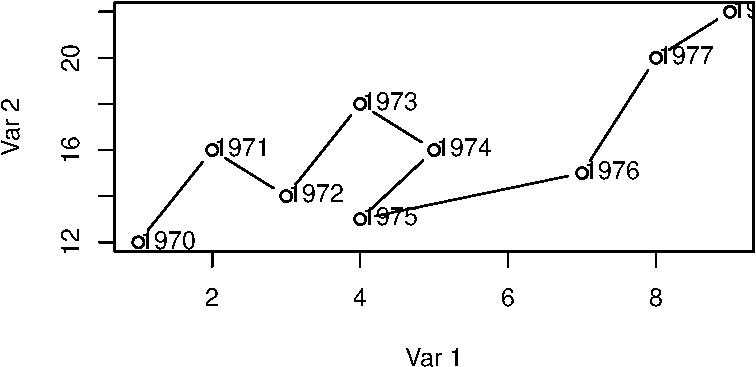
\includegraphics{_main_files/figure-latex/unnamed-chunk-87-1.pdf}

\begin{enumerate}
\def\labelenumi{(\arabic{enumi})}
\setcounter{enumi}{21}
\tightlist
\item
  and 23. \emph{(This task is worth 10 points)}
  The following chart shows the simultaneous development of the unemployment rate and GDP per capita over time for \textbf{France}.
\end{enumerate}

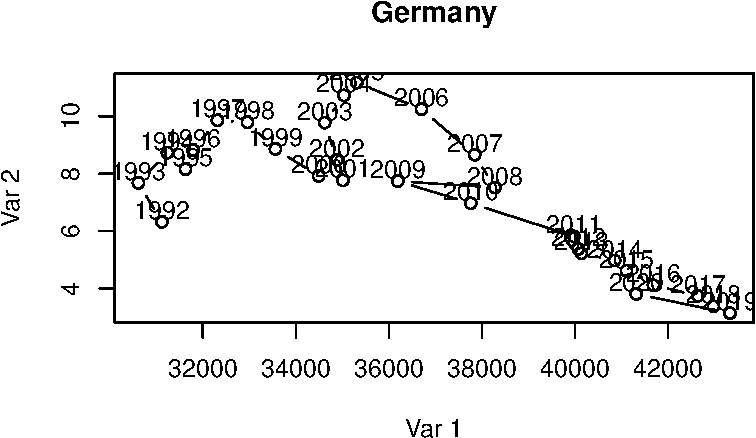
\includegraphics{_main_files/figure-latex/unnamed-chunk-88-1.pdf}

Suppose you want to visualize the simultaneous evolution of the unemployment rate and GDP per capita over time for Germany as well.\\
Suppose further that you have found the following lines of code that create the kind of chart you are looking for.

\begin{Shaded}
\begin{Highlighting}[]
\CommentTok{\# Data}
\NormalTok{x }\OtherTok{\textless{}{-}} \FunctionTok{c}\NormalTok{(}\DecValTok{1}\NormalTok{, }\DecValTok{2}\NormalTok{, }\DecValTok{3}\NormalTok{, }\DecValTok{4}\NormalTok{, }\DecValTok{5}\NormalTok{, }\DecValTok{4}\NormalTok{, }\DecValTok{7}\NormalTok{, }\DecValTok{8}\NormalTok{, }\DecValTok{9}\NormalTok{)}
\NormalTok{y }\OtherTok{\textless{}{-}} \FunctionTok{c}\NormalTok{(}\DecValTok{12}\NormalTok{, }\DecValTok{16}\NormalTok{, }\DecValTok{14}\NormalTok{, }\DecValTok{18}\NormalTok{, }\DecValTok{16}\NormalTok{, }\DecValTok{13}\NormalTok{, }\DecValTok{15}\NormalTok{, }\DecValTok{20}\NormalTok{, }\DecValTok{22}\NormalTok{)}
\NormalTok{labels }\OtherTok{\textless{}{-}} \DecValTok{1970}\SpecialCharTok{:}\DecValTok{1978}

\CommentTok{\# Connected scatter plot with text}
\FunctionTok{plot}\NormalTok{(x, y, }\AttributeTok{type =} \StringTok{"b"}\NormalTok{, }\AttributeTok{xlab =} \StringTok{"Var 1"}\NormalTok{, }\AttributeTok{ylab =} \StringTok{"Var 2"}\NormalTok{); }\FunctionTok{text}\NormalTok{(x }\SpecialCharTok{+} \FloatTok{0.4}\NormalTok{, y }\SpecialCharTok{+} \FloatTok{0.1}\NormalTok{, labels) }
\end{Highlighting}
\end{Shaded}

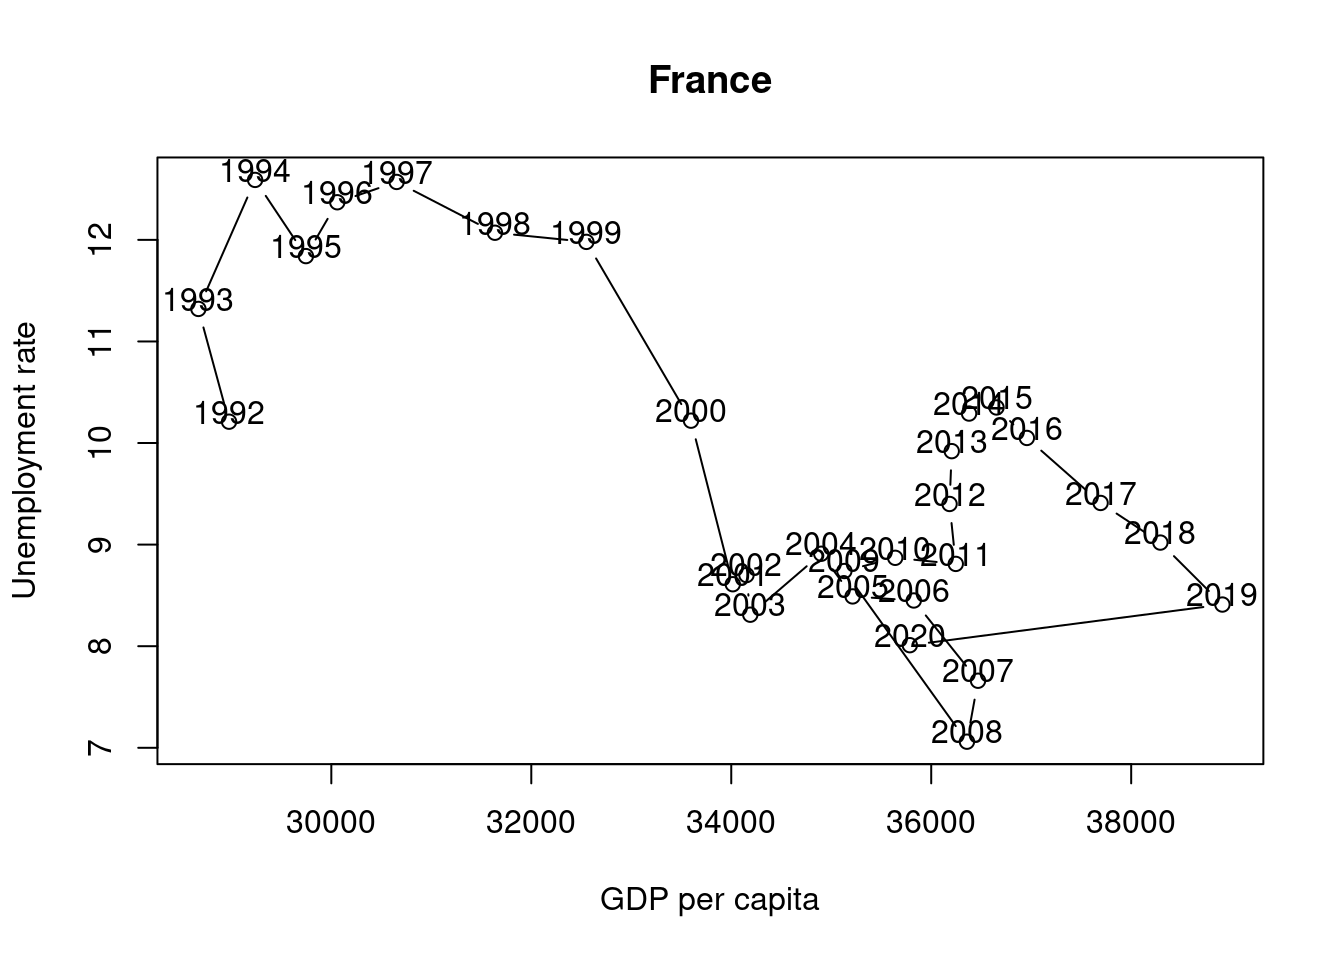
\includegraphics{_main_files/figure-latex/unnamed-chunk-89-1.pdf}

Use these lines of code and customize them to create the co-movement visualization for \textbf{Germany} using the available `df' data.
The result should look something like this:

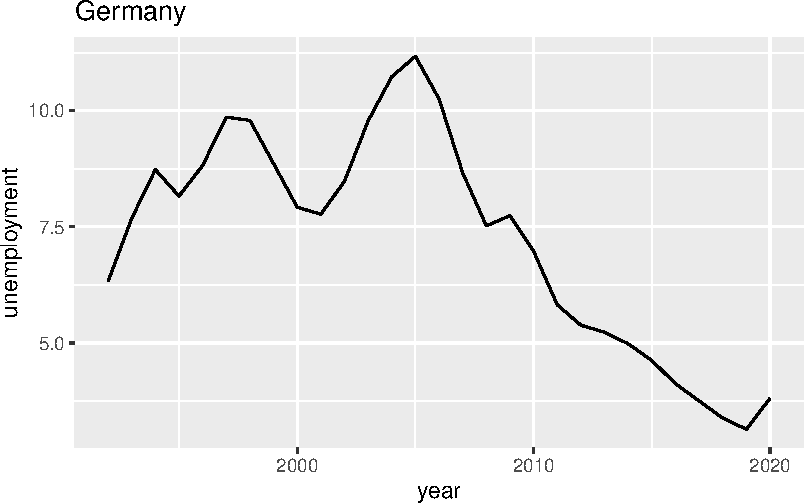
\includegraphics{_main_files/figure-latex/unnamed-chunk-90-1.pdf}

\begin{enumerate}
\def\labelenumi{(\arabic{enumi})}
\setcounter{enumi}{23}
\tightlist
\item
  Interpret the two graphs above, which show the simultaneous evolution of the unemployment rate and GDP per capita over time for Germany and France. What are your expectations regarding the correlation between the unemployment rate and GDP per capita variables? Can you see this expectation in the figures? Discuss.
\end{enumerate}

Please find solutions \href{https://raw.githubusercontent.com/hubchev/courses/main/scr/un_gdp_ger_fra.R}{here}.

\begin{exercise}
\protect\hypertarget{exr:hortacsu}{}\label{exr:hortacsu}Import data and write a report

Reproduce Figure 3 of \citet[p.~99]{Hortacsu2015Ongoing} using R. Write a clear report about your work, i.e., document everything with a R script or a R Markdown file.

Here are the required steps:

\begin{enumerate}
\def\labelenumi{\arabic{enumi}.}
\tightlist
\item
  Go to \url{https://www.aeaweb.org/articles?id=10.1257/jep.29.4.89} and download the \emph{replication package} from the \emph{OPENICPSR} page. Please note, that you can download the replication package after you have registered for the platform.
\item
  Unzip the replication package.
\item
  In the file \emph{diffusion\_curves\_figure.xlsx} you find the required data. Import them to R.
\item
  Reproduce the plot using ggplot().
\end{enumerate}

Please find solutions \href{https://raw.githubusercontent.com/hubchev/courses/main/scr/hortacsu_figure_3.R}{here}.
\end{exercise}

\hypertarget{write-with-r-markdown}{%
\chapter{Write with R Markdown}\label{write-with-r-markdown}}

\begin{figure}
\centering
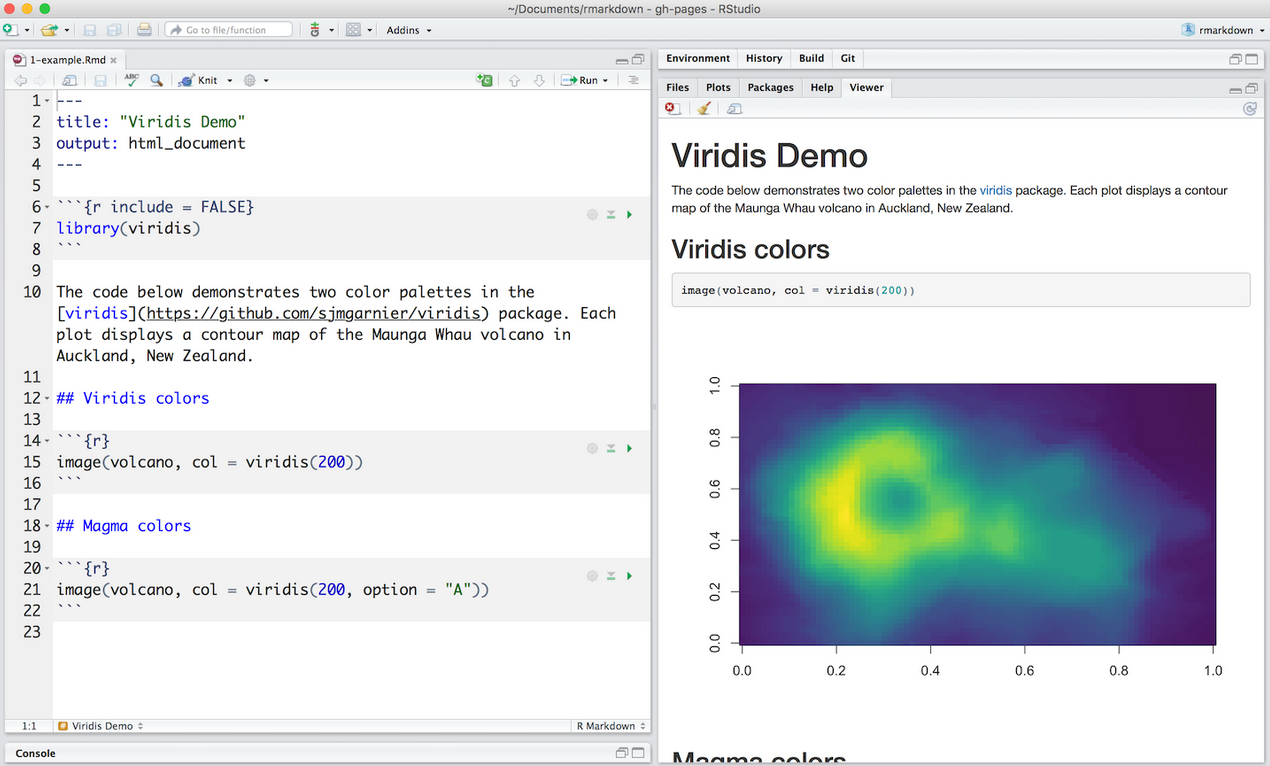
\includegraphics[width=0.75\textwidth,height=\textheight]{fig/rmstudio.png}
\caption{\label{fig:examplermd} Example of an R Markdown file}
\end{figure}

R Markdown provides an authoring framework for data science. You can use a single
R Markdown file to transcript your work, run code, and generate high quality reports, books, websites, articles, theses, blogs, and many more.

In contrast to Quarto (see: \url{https://quarto.org} and \url{https://quarto.org/docs/get-started/hello/rstudio.html}), which is the more recent format, R Markdown is around for some time and hence there are uncountable resources to learn it. For example:

\begin{itemize}
\tightlist
\item
  The \href{https://raw.githubusercontent.com/rstudio/cheatsheets/main/rmarkdown.pdf}{R Markdown Cheatsheet} from posit offers an overview on the most important features of R Markdown.
\end{itemize}

\begin{figure}
\centering
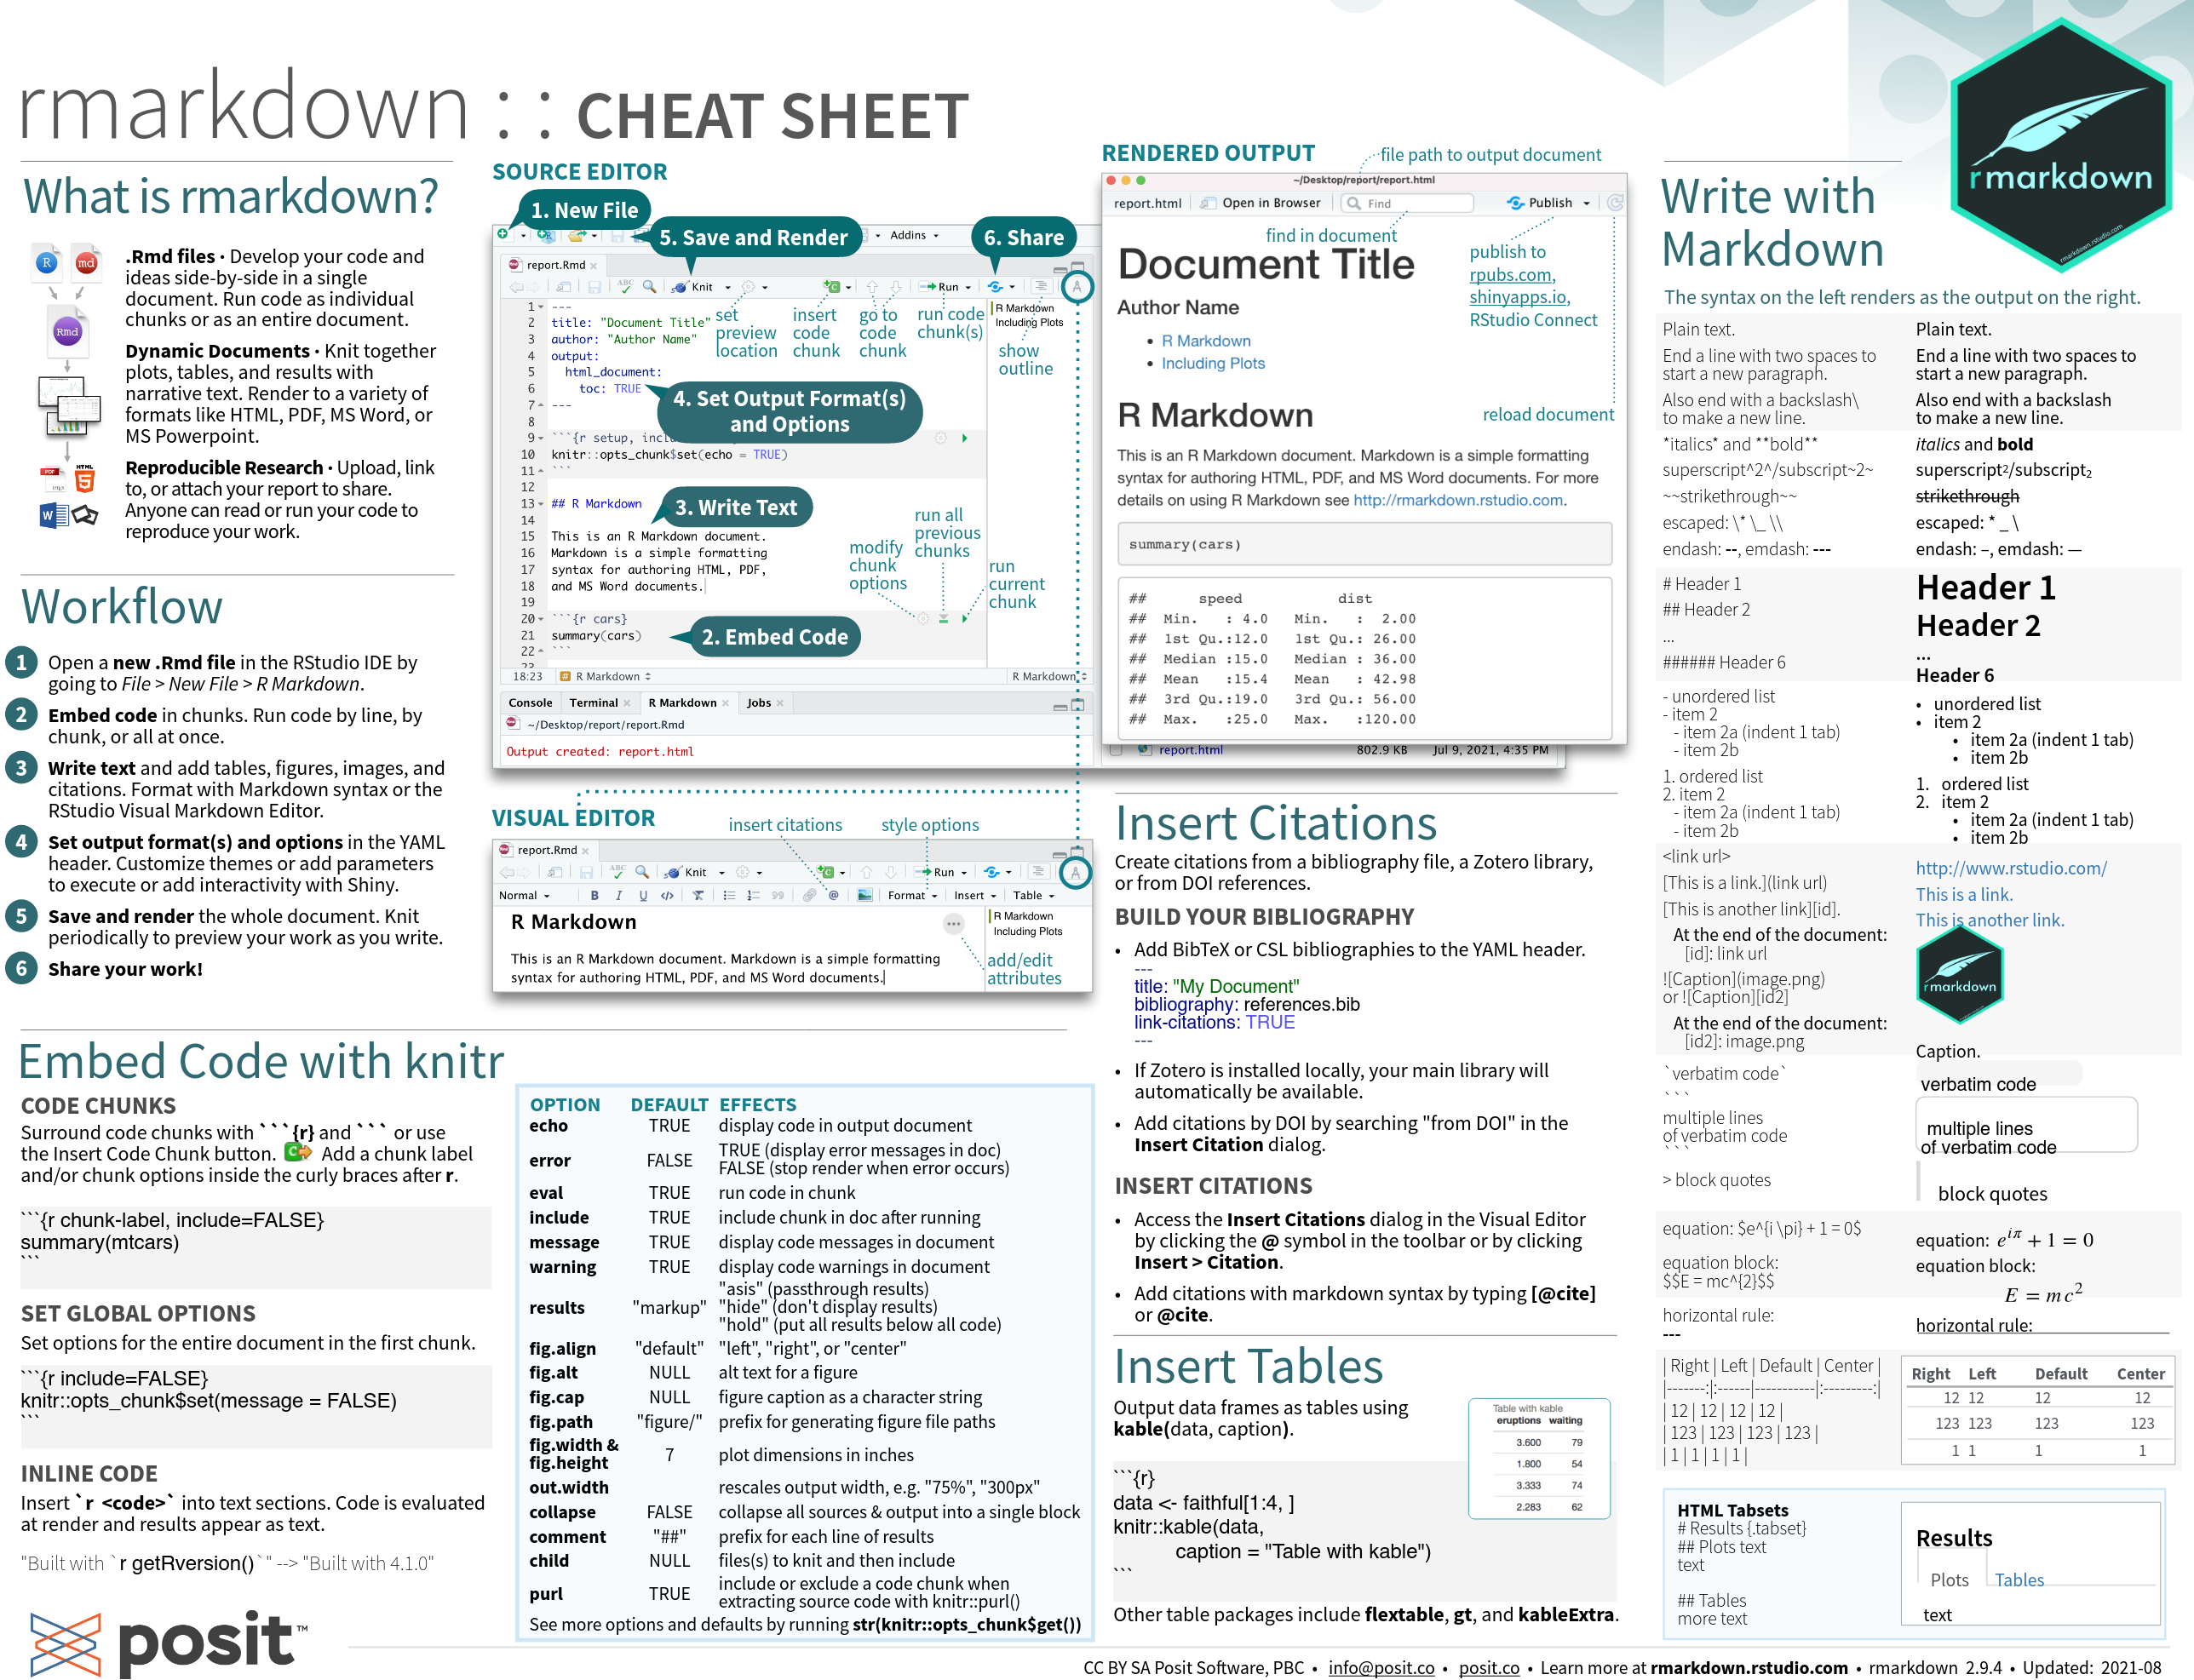
\includegraphics[width=0.5\textwidth,height=\textheight]{fig/rmdcheat.png}
\caption{\label{fig:rmdcheat} R Markdown Cheatsheet from posit}
\end{figure}

\begin{itemize}
\tightlist
\item
  The book \emph{R Markdown Cookbook} by \citet{Xie2020R} offers an introduction. The \href{https://bookdown.org/yihui/rmarkdown-cookbook}{online version of the book} is regularly updated and free of costs.
\end{itemize}

\begin{figure}
\centering

\includegraphics[width=0.25\textwidth,height=\textheight]{fig/rmarkdownbook.png}
\caption{\citet{Xie2020R}: R Markdown Cookbook}
\end{figure}

\begin{itemize}
\tightlist
\item
  The book \emph{R Markdown: The Definitive Guide} by \citet{Xie2018R} offers a comprehensive introduction. \href{https://bookdown.org/yihui/rmarkdown}{The online version of the book} is regularly updated and free of costs.
\end{itemize}

\begin{figure}
\centering
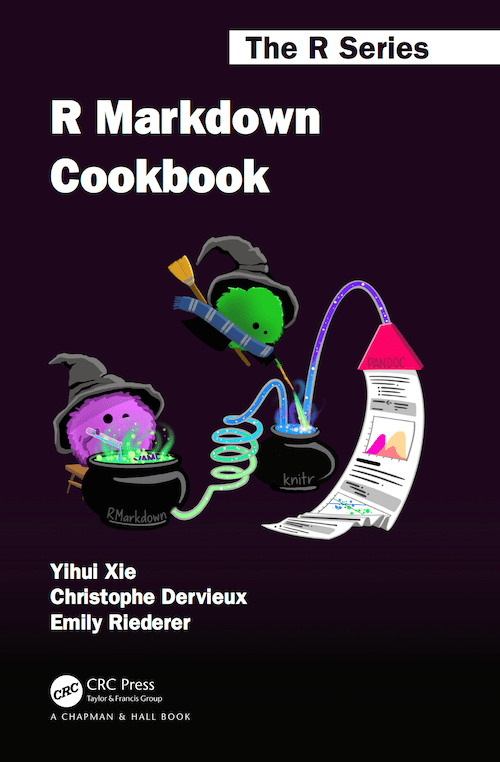
\includegraphics[width=0.25\textwidth,height=\textheight]{fig/rmcb.png}
\caption{\citet{Xie2018R}: R Markdown: The Definitive Guide}
\end{figure}

Please watch the video \href{https://vimeo.com/178485416}{What is R Markdown?} and then study the \href{https://rmarkdown.rstudio.com/lesson-1.html}{R Markdown tutorial from RStudio}.

\begin{exercise}
\protect\hypertarget{exr:rmdfirst}{}\label{exr:rmdfirst}

Start Markdown and R Markdown

\begin{enumerate}
\def\labelenumi{\alph{enumi})}
\tightlist
\item
  You can learn Markdown (not R Markdown!) in 10 minutes. Just go to \url{https://www.markdowntutorial.com} and work throught the interactive lessons.
\item
  Now create your first R Markdown file in 3 minutes by doing the following:
\end{enumerate}

\begin{itemize}
\tightlist
\item
  click in RStudio on \emph{File \textgreater{} New File \textgreater{} R Markdown}
\item
  click \emph{OK}
\item
  look for a button entitled \emph{Knit} and click it
\item
  save your file (it will be saved with .Rmd file extension)
\end{itemize}

\begin{enumerate}
\def\labelenumi{\alph{enumi})}
\setcounter{enumi}{2}
\tightlist
\item
  Play around with the file. For example, change the output format can you create a word file or a presentation. Play around with the code chunks. Add a picture that you find somewhere online.
\item
  Set your working directory to the folder where you have saved your first Rmd-file. Can you come up with a way to generate different output format with just one function.
\end{enumerate}

\end{exercise}

\begin{exercise}
\protect\hypertarget{exr:rmdapa}{}\label{exr:rmdapa}

R Markdown APA template

\begin{enumerate}
\def\labelenumi{\alph{enumi})}
\tightlist
\item
  Create a new R Markdown file (\emph{File \textgreater{} New File \textgreater{} R Markdown}), save the file in an empty folder, and knit it.
\item
\end{enumerate}

\begin{itemize}
\tightlist
\item
  Make a new script with \emph{File \textgreater{} New File \textgreater{} R Script}.
\item
  Go to \url{https://scholar.google.de/} and search for \emph{osrmtime}.
\item
  Click on \emph{``cite''} and \emph{``BibTeX''}. Copy and paste everything that you see into your script and save the script as \emph{lit.bib}. R Studio will ask you if you confirm the file type change. Click yes.
\item
  Add the text \emph{``bibliography: references.bib''} to your YAML header of your R Markdown file so that it looks somehow like that:
\end{itemize}

\end{exercise}

\begin{Shaded}
\begin{Highlighting}[]
\NormalTok{title: "Untitled"}
\NormalTok{author: "Stephan Huber"}
\NormalTok{date: "\textasciigrave{}r Sys.Date()\textasciigrave{}"}
\NormalTok{output: html\_document}
\NormalTok{bibliography: lit.bib}
\end{Highlighting}
\end{Shaded}

\begin{itemize}
\tightlist
\item
  Now you can cite the OSRMTIME paper with \texttt{@huber2016calculate} somewhere in the text of your R Markdown file.
\item
  Knit the R Markdown file and you should see the paper cited and a reference list at the end of the html report.
\item
  You can manipulate the citation style you can specify a CSL (Citation Style Language) file in the YAML header. For example the APA style can be chosen with:
\end{itemize}

\begin{Shaded}
\begin{Highlighting}[]
\NormalTok{csl: "https://raw.githubusercontent.com/citation{-}style{-}language/styles/master/apa.csl"}
\end{Highlighting}
\end{Shaded}

Many more citation styles can be found \href{https://github.com/citation-style-language/styles}{here}.

\begin{exercise}
\protect\hypertarget{exr:rmdsecond}{}\label{exr:rmdsecond}

R Markdown template

Please follow the instructions below to access the file ``23-09\_ds-project-desc.Rmd'' from my GitHub account:

\begin{enumerate}
\def\labelenumi{\arabic{enumi}.}
\tightlist
\item
  Download the file from my GitHub account by clicking on the link provided here.
\item
  Save the file in your working directory.
\item
  Use the knit function to run the file, but be aware that it may not work properly at first. If you encounter any issues, troubleshooting may be required. Don`t worry, error messages will usually provide guidance to help you resolve the issue. Please note that the YAML header is sensitive to spacing, so be careful when setting it up to avoid breaking the code.
\item
  In the project template, I have used BibTeX to cite literature. This method is excellent for automating tedious tasks such as citing papers and generating reference lists based on citation styles, saving time and reducing the likelihood of citation errors. The literature cited is in a separate file, which can be found on one of my GitHub repositories.
\end{enumerate}

\end{exercise}

\hypertarget{appendix}{%
\chapter{Appendix}\label{appendix}}

\hypertarget{helpful-shortcuts}{%
\section{Helpful shortcuts}\label{helpful-shortcuts}}

\begin{longtable}[]{@{}rl@{}}
\caption{Table 1: Different OS, different keys}\tabularnewline
\toprule\noalign{}
Key in Windows/Linux & Key in Mac \\
\midrule\noalign{}
\endfirsthead
\toprule\noalign{}
Key in Windows/Linux & Key in Mac \\
\midrule\noalign{}
\endhead
\bottomrule\noalign{}
\endlastfoot
CTRL & Command Key \\
Alt & Option Key \\
\end{longtable}

\begin{longtable}[]{@{}
  >{\raggedright\arraybackslash}p{(\columnwidth - 4\tabcolsep) * \real{0.1562}}
  >{\raggedright\arraybackslash}p{(\columnwidth - 4\tabcolsep) * \real{0.2062}}
  >{\raggedright\arraybackslash}p{(\columnwidth - 4\tabcolsep) * \real{0.6375}}@{}}
\caption{Table 2: Helpful shortcuts}\tabularnewline
\toprule\noalign{}
\begin{minipage}[b]{\linewidth}\raggedright
Action
\end{minipage} & \begin{minipage}[b]{\linewidth}\raggedright
Shortcut Keys
\end{minipage} & \begin{minipage}[b]{\linewidth}\raggedright
Description
\end{minipage} \\
\midrule\noalign{}
\endfirsthead
\toprule\noalign{}
\begin{minipage}[b]{\linewidth}\raggedright
Action
\end{minipage} & \begin{minipage}[b]{\linewidth}\raggedright
Shortcut Keys
\end{minipage} & \begin{minipage}[b]{\linewidth}\raggedright
Description
\end{minipage} \\
\midrule\noalign{}
\endhead
\bottomrule\noalign{}
\endlastfoot
Run code & Ctrl + Enter & Runs the current line and jumps to the next one, or runs the selected part without jumping further. \\
& Alt + Enter & Allows running code without moving the cursor to the next line if you want to run one line of code multiple times without selecting it. \\
& Ctrl + Alt + R & Runs the entire script. \\
& Ctrl + Alt + B/E & Run the script from the Beginning to the current line and from the current line to the End. \\
Write code & Alt + (-) & Inserts the assignment operator (\textless-) with spaces surrounding it. \\
& Ctrl + Shift + M & Inserts the magrittr/pipe operator (\%\textgreater\%) with spaces surrounding it. \\
& Ctrl + Shift + C & Comments out code by putting a \texttt{\#} in front of each line of marked code of a script. \\
& Ctrl + Shift + R & Creates a foldable comment section in your code. \\
Navigating in RStudio & Ctrl + 1 & Move focus to editor. \\
& Ctrl + 2 & Move focus to console. \\
& Ctrl+Tab and Ctrl+Shift+Tab & to switch between tabs. \\
& Ctrl + Shift + N & Open a new R script. \\
& Ctrl + w & Close a tab. \\
\end{longtable}

\hypertarget{sec:navigation}{%
\section{Navigating the file system}\label{sec:navigation}}

It is essential to know how R interacts with the file system on your computer. Modern operating systems are incredibly user-friendly and try to hide boring and annoying stuff from the customer. In the following, I will try to give a brief introduction on how to navigate around a computer using a DOS or UNIX shell. If you familiar with that, you can skip this part of the notes.

\hypertarget{sec:filesystem}{%
\subsection{The file system}\label{sec:filesystem}}

In this section, I describe the basic idea behind file locations and file paths. Regardless of whether you are using Windows, macOS, or Linux, every file on the computer is assigned a human-readable address, and every address has the same basic structure: it describes a path that starts from a root location, through a series of folders (or directories), and finally ends up at the file.

On a Windows computer, the root is the storage device on which the file is stored, and for many home computers, the name of the storage device that stores all your files is \texttt{C:}. After that comes the folders, and on Windows, the folder names are separated by a backslash symbol \texttt{\textbackslash{}}. So, the complete path to this book on my Windows computer might be something like this:

\begin{verbatim}
C:\Users\huber\Rbook\rcourse-book.pdf
\end{verbatim}

On Linux, Unix, and macOS systems, the addresses look a little different, but they are more or less identical in spirit. Instead of using the backslash, folders are separated using a forward slash, and unlike Windows, they do not treat the storage device as being the root of the file system. So, the path on a Mac might be something like this:

/Users/huber/Rbook/rcourse-book.pdf

That is what we mean by the \emph{path} to a file. The next concept to grasp is the idea of a working directory and how to change it. For those of you who have used command-line interfaces previously, this should be obvious already. But if not, here is what I mean. The working directory is just whatever folder I am currently looking at. Suppose that I am currently looking for files in Explorer (if you are using Windows) or using Finder (on a Mac). The folder I currently have open is my user directory (i.e., \texttt{C:\textbackslash{}Users\textbackslash{}huber} or \texttt{/Users/huber}). That is my current working directory.

\hypertarget{working-directory}{%
\subsection{Working directory}\label{working-directory}}

The next concept to grasp is the idea of a \emph{working directory} and how to change it. For those of you who have used command line interfaces previously, this should be obvious already. But if not, here's what I mean. The working directory is just ``whatever folder I'm currently looking at''. Suppose that I'm currently looking for files in Explorer (if you're using Windows) or using Finder (on a Mac). The folder I currently have open is my user directory (i.e., \texttt{C:\textbackslash{}Users\textbackslash{}huber} or \texttt{/Users/huber}). That's my current working directory.

The fact that we can imagine that the program is ``in'' a particular directory means that we can talk about moving \emph{from} our current location \emph{to} a new one. What that means is that we might want to specify a new location in relation to our current location. To do so, we need to introduce two new conventions. Regardless of what operating system you're using, we use \texttt{.} to refer to the current working directory, and \texttt{..} to refer to the directory above it. This allows us to specify a path to a new location in relation to our current location, as the following examples illustrate. Let's assume that I'm using my Windows computer, and my working directory is \texttt{C:\textbackslash{}Users\textbackslash{}huber\textbackslash{}Rbook}. The table below shows several addresses in relation to my current one:

\begin{longtable}[]{@{}ll@{}}
\toprule\noalign{}
Absolute path & Relative path \\
\midrule\noalign{}
\endhead
\bottomrule\noalign{}
\endlastfoot
\texttt{C:\textbackslash{}Users\textbackslash{}huber} & \texttt{..} \\
\texttt{C:\textbackslash{}Users} & \texttt{..\textbackslash{}..} \\
\texttt{C:\textbackslash{}Users\textbackslash{}huber\textbackslash{}Rbook\textbackslash{}source} & \texttt{.\textbackslash{}source} \\
\texttt{C:\textbackslash{}Users\textbackslash{}huber\textbackslash{}nerdstuff} & \texttt{..\textbackslash{}nerdstuff} \\
\end{longtable}

It is quite common on computers that have multiple users to define \texttt{\textasciitilde{}} to be the user's \emph{home directory}. The home directory on a Mac for the `\texttt{huber\textquotesingle{}\textquotesingle{}\ user\ is}/Users/huber/\texttt{.\ And\ so,\ not\ surprisingly,\ it\ is\ possible\ to\ define\ other\ directories\ in\ terms\ of\ their\ relationship\ to\ the\ home\ directory.\ For\ example,\ an\ alternative\ way\ to\ describe\ the\ location\ of\ the}rcourse-book.pdf` file on a Mac would be

\begin{verbatim}
~\Rbook\rcourse-book.pdf
\end{verbatim}

You can find out your home directory with the \texttt{path.expand()} function:

\begin{Shaded}
\begin{Highlighting}[]
\FunctionTok{path.expand}\NormalTok{(}\StringTok{"\textasciitilde{}"}\NormalTok{)}
\end{Highlighting}
\end{Shaded}

\begin{verbatim}
## [1] "/home/sthu"
\end{verbatim}

Thus, on my machine \textasciitilde{} is an abbreviation for the path /home/sthu.

\begin{Shaded}
\begin{Highlighting}[]
\FunctionTok{getwd}\NormalTok{()}
\end{Highlighting}
\end{Shaded}

\begin{verbatim}
## [1] "/home/sthu/Dropbox/hsf/courses/ds"
\end{verbatim}

\hypertarget{sec:navigationR}{%
\subsection{Navigating the file system using the R console}\label{sec:navigationR}}

When you want to load or save a file in R it's important to know what the working directory is. You can find out by using the \texttt{getwd()} command. For the moment, let's assume that I'm using Mac OS or Linux, since things are different on Windows, see section \ref{sec:winbackslash}.
Let's check the current active working directory:

\begin{Shaded}
\begin{Highlighting}[]
\FunctionTok{getwd}\NormalTok{()}
\end{Highlighting}
\end{Shaded}

\begin{verbatim}
## [1] "/home/sthu/Dropbox/hsf/courses/ds"
\end{verbatim}

The function \texttt{setwd()} allows to change the working directory:

\begin{Shaded}
\begin{Highlighting}[]
\FunctionTok{setwd}\NormalTok{(}\StringTok{"/Users/huber/Rbook/data"}\NormalTok{)}
\FunctionTok{setwd}\NormalTok{(}\StringTok{"./Rbook/data"}\NormalTok{)}
\end{Highlighting}
\end{Shaded}

The function \texttt{list.files()} lists all the files in that directory:

\begin{Shaded}
\begin{Highlighting}[]
\FunctionTok{list.files}\NormalTok{()}
\end{Highlighting}
\end{Shaded}

\hypertarget{sec:rstudioprojects}{%
\subsection{R Studio projects}\label{sec:rstudioprojects}}

Setting the working directory repeatedly can be a cumbersome task. Fortunately, R Studio projects can automate this process for you. When you open an R Studio project, the working directory is automatically set to the project directory.

Creating a new project in R Studio is simple. Just click on \emph{File \textgreater{} New Project\ldots{}}. This will create a directory on your computer with a \_*.Rproj\_ file that can be used to open the saved project at a later date. The newly created directory contains your R code, data files, and other project-related files. By working within projects, all of your files and data are organized in one place, making it easier to share your work with others, reproduce your analyses, and keep track of changes over time.

\hypertarget{sec:winbackslash}{%
\subsection{Why do the Windows paths use the back-slash?}\label{sec:winbackslash}}

Let's suppose I'm using a computer with Windows. As before, I can find out what my current working directory is like this:

\begin{Shaded}
\begin{Highlighting}[]
\FunctionTok{getwd}\NormalTok{()}
\NormalTok{[}\DecValTok{1}\NormalTok{] }\StringTok{"C:/Users/huber/}
\end{Highlighting}
\end{Shaded}

R is displaying a Windows path using the wrong type of slash, the back-slash. The answer has to do with the fact that R treats the \texttt{\textbackslash{}} character as \emph{special}. If you're deeply wedded to the idea of specifying a path using the Windows style slashes, then what you need to use two back-slashes \texttt{\textbackslash{}\textbackslash{}} whenever you mean \texttt{\textbackslash{}}. In other words, if you want to specify the working directory on a Windows computer, you need to use one of the following commands:

\begin{Shaded}
\begin{Highlighting}[]
\FunctionTok{setwd}\NormalTok{( }\StringTok{"C:/Users/huber"}\NormalTok{ )}
\FunctionTok{setwd}\NormalTok{( }\StringTok{"C:}\SpecialCharTok{\textbackslash{}\textbackslash{}}\StringTok{Users}\SpecialCharTok{\textbackslash{}\textbackslash{}}\StringTok{huber"}\NormalTok{ )}
\end{Highlighting}
\end{Shaded}

\hypertarget{troubleshooting}{%
\section{Troubleshooting}\label{troubleshooting}}

Troubleshooting is perhaps the most important skill for a data scientist. To tackle problems effectively, you need to understand them, replicate them, and then work to solve them. To help you with this process, here are some guidelines:

When seeking help, be sure to provide information about your machine, including the operating system, the version of R, and the packages you have loaded. You can use the sessionInfo() function to gather this information. Here's an example from my machine:

\begin{Shaded}
\begin{Highlighting}[]
\FunctionTok{sessionInfo}\NormalTok{()}
\end{Highlighting}
\end{Shaded}

\begin{verbatim}
## R version 4.3.1 (2023-06-16)
## Platform: x86_64-pc-linux-gnu (64-bit)
## Running under: Debian GNU/Linux 12 (bookworm)
## 
## Matrix products: default
## BLAS:   /usr/lib/x86_64-linux-gnu/blas/libblas.so.3.11.0 
## LAPACK: /usr/lib/x86_64-linux-gnu/lapack/liblapack.so.3.11.0
## 
## locale:
##  [1] LC_CTYPE=en_US.UTF-8       LC_NUMERIC=C               LC_TIME=en_US.UTF-8        LC_COLLATE=en_US.UTF-8    
##  [5] LC_MONETARY=en_US.UTF-8    LC_MESSAGES=en_US.UTF-8    LC_PAPER=en_US.UTF-8       LC_NAME=C                 
##  [9] LC_ADDRESS=C               LC_TELEPHONE=C             LC_MEASUREMENT=en_US.UTF-8 LC_IDENTIFICATION=C       
## 
## time zone: Europe/Berlin
## tzcode source: system (glibc)
## 
## attached base packages:
## [1] stats     graphics  grDevices utils     datasets  methods   base     
## 
## other attached packages:
##  [1] dplyr_1.1.2          papaja_0.1.2.9000    tinylabels_0.2.4     sjPlot_2.8.15        ggpubr_0.6.0        
##  [6] datasauRus_0.1.6     haven_2.5.3          janitor_2.2.0        wbstats_1.0.4        scales_1.2.1        
## [11] lubridate_1.9.3      forcats_1.0.0        purrr_1.0.2          readr_2.1.4          tidyr_1.3.0         
## [16] tibble_3.2.1         ggplot2_3.4.3        tidyverse_2.0.0      stringr_1.5.0        bundesligR_0.1.0    
## [21] knitr_1.42           pacman_0.5.1         captioner_2.2.3.9000
## 
## loaded via a namespace (and not attached):
##   [1] rstudioapi_0.15.0         jsonlite_1.8.4            datawizard_0.9.0          magrittr_2.0.3           
##   [5] TH.data_1.1-2             estimability_1.4.1        farver_2.1.1              nloptr_2.0.3             
##   [9] rmarkdown_2.21            fs_1.6.2                  ragg_1.2.5                vctrs_0.6.3              
##  [13] memoise_2.0.1             minqa_1.2.6               effectsize_0.8.6          tinytex_0.45             
##  [17] rstatix_0.7.2             htmltools_0.5.5           usethis_2.1.6             curl_5.1.0               
##  [21] broom_1.0.5               sjmisc_2.8.9              sass_0.4.6                bslib_0.4.2              
##  [25] htmlwidgets_1.6.2         sandwich_3.0-2            emmeans_1.8.8             zoo_1.8-12               
##  [29] cachem_1.0.8              mime_0.12                 lifecycle_1.0.3           pkgconfig_2.0.3          
##  [33] sjlabelled_1.2.0          Matrix_1.6-1.1            R6_2.5.1                  fastmap_1.1.1            
##  [37] shiny_1.7.4               snakecase_0.11.1          digest_0.6.31             colorspace_2.1-0         
##  [41] ps_1.7.5                  pkgload_1.3.2             textshaping_0.3.6         labeling_0.4.2           
##  [45] fansi_1.0.4               timechange_0.2.0          httr_1.4.7                abind_1.4-5              
##  [49] compiler_4.3.1            remotes_2.4.2             withr_2.5.0               backports_1.4.1          
##  [53] carData_3.0-5             sylly_0.1-6               performance_0.10.5        koRpus_0.13-8            
##  [57] pkgbuild_1.4.0            highr_0.10                ggsignif_0.6.4            MASS_7.3-60              
##  [61] sjstats_0.18.2            sessioninfo_1.2.2         tools_4.3.1               httpuv_1.6.11            
##  [65] glue_1.6.2                callr_3.7.3               nlme_3.1-162              promises_1.2.0.1         
##  [69] grid_4.3.1                generics_0.1.3            gtable_0.3.3              tzdb_0.4.0               
##  [73] data.table_1.14.8         hms_1.1.3                 car_3.1-2                 utf8_1.2.3               
##  [77] pillar_1.9.0              later_1.3.1               splines_4.3.1             lattice_0.20-45          
##  [81] survival_3.5-3            tidyselect_1.2.0          miniUI_0.1.1.1            bookdown_0.35            
##  [85] xfun_0.40                 devtools_2.4.5            stringi_1.7.12            yaml_2.3.7               
##  [89] boot_1.3-28.1             evaluate_0.22             codetools_0.2-19          cli_3.6.1                
##  [93] parameters_0.21.2         xtable_1.8-4              systemfonts_1.0.4         munsell_0.5.0            
##  [97] processx_3.8.1            jquerylib_0.1.4           modelr_0.1.11             Rcpp_1.0.10              
## [101] ggeffects_1.3.1           wordcountaddin_0.3.0.9000 coda_0.19-4               ellipsis_0.3.2           
## [105] prettyunits_1.1.1         bayestestR_0.13.1         profvis_0.3.8             urlchecker_1.0.1         
## [109] lme4_1.1-34               mvtnorm_1.2-3             insight_0.19.5            crayon_1.5.2             
## [113] rlang_1.1.1               multcomp_1.4-25
\end{verbatim}

  \bibliography{book.bib}

\end{document}
